% -*- Mode:TeX -*-

%% IMPORTANT: The official thesis specifications are available at:
%%
%%            Please verify your thesis' formatting and copyright
%%            assignment before submission.  If you notice any
%%            discrepancies between these templates and the
%%            MIT Libraries' specs, please let us know
%%            by e-mailing thesis@mit.edu

%% The documentclass options along with the pagestyle can be used to generate
%% a technical report, a draft copy, or a regular thesis.  You may need to
%% re-specify the pagestyle after you \include  cover.tex.  For more
%% information, see the first few lines of mitthesis.cls. 

%\documentclass[12pt,vi,twoside]{mitthesis}
%%
%%  If you want your thesis copyright to you instead of MIT, use the
%%  ``vi'' option, as above.
%%
%\documentclass[12pt,twoside,leftblank]{mitthesis}
%%
%% If you want blank pages before new chapters to be labelled ``This
%% Page Intentionally Left Blank'', use the ``leftblank'' option, as
%% above. 
% Add all your packages here


\documentclass[12pt,twoside]{mitthesis}
\usepackage{enumerate}
\usepackage{graphicx} 
%\def\spanishoptions{mexico}
%\usepackage[spanish]{babel}
%\usepackage[T1]{fontenc}
%\usepackage[utf8]{inputenc}
\usepackage{amsmath} 
\usepackage{lgrind}
\usepackage{listings}
\usepackage{color}
\usepackage{float}
\usepackage{placeins}
\usepackage{times}


\usepackage{ifxetex}

\ifxetex
  \usepackage{fontspec}
\else
  \usepackage[T1]{fontenc}
  \usepackage[utf8]{inputenc}
  \usepackage{lmodern}
\fi

\usepackage{caption}
%\DeclareCaptionFormat{myformat}{#1#2#3}
\newlength\myindention
\DeclareCaptionFormat{myformat}%
{#1#2#3 \hspace*{\myindention}}
\captionsetup{format=myformat}
\captionsetup[lstlisting]{position=bottom,format=myformat}
\renewcommand{\lstlistingname}{Algoritmo}

\usepackage{fancyhdr}
\pagestyle{fancy}

\fancyhead{}
\fancyfoot{}

%\fancyhead[RO,RE]{\fontsize{10}{12} \selectfont \thepage}
\fancyhead[LO]{\fontsize{10}{12} \selectfont \leftmark}
\fancyhead[LE]{\fontsize{10}{12} \selectfont \leftmark}

\renewcommand{\headrulewidth}{0.0pt}
\renewcommand{\footrulewidth}{0.0pt}

%\addto\captionsspanish{%
%  \renewcommand{\appendixname}%
%    {Anexos}%
%}

\usepackage{blindtext}
\usepackage{etoolbox}
\patchcmd{\chapter}{plain}{fancy}{}{}

%\usepackage{fontspec}
%\setmainfont{Times New Roman}
%\setmainfont{Arial}


%\usepackage[T1,T2A]{fontenc}
%\usepackage[latin1]{inputenc}
%\usepackage[spanish]{babel}

%\selectlanguage{spanish}

%\pagestyle{plain}
 
%% This bit allows you to either specify only the files which you wish to
%% process, or `all' to process all files which you \include.
%% Krishna Sethuraman (1990).

% \typein [\files]{Enter file names to process, (chap1,chap2 ...), or
%  `all' to process all files:}
\def\all{all}
% \ifx\files\all \typeout{Including all files.} \else \typeout{Including only \files.} \includeonly{\files} \fi

\begin{document}

% -*-latex-*-
% 
% For questions, comments, concerns or complaints:
% thesis@mit.edu
% 
%
% $Log: cover.tex,v $
% Revision 1.8  2008/05/13 15:02:15  jdreed
% Degree month is June, not May.  Added note about prevdegrees.
% Arthur Smith's title updated
%
% Revision 1.7  2001/02/08 18:53:16  boojum
% changed some \newpages to \cleardoublepages
%
% Revision 1.6  1999/10/21 14:49:31  boojum
% changed comment referring to documentstyle
%
% Revision 1.5  1999/10/21 14:39:04  boojum
% *** empty log message ***
%
% Revision 1.4  1997/04/18  17:54:10  othomas
% added page numbers on abstract and cover, and made 1 abstract
% page the default rather than 2.  (anne hunter tells me this
% is the new institute standard.)
%
% Revision 1.4  1997/04/18  17:54:10  othomas
% added page numbers on abstract and cover, and made 1 abstract
% page the default rather than 2.  (anne hunter tells me this
% is the new institute standard.)
%
% Revision 1.3  93/05/17  17:06:29  starflt
% Added acknowledgements section (suggested by tompalka)
% 
% Revision 1.2  92/04/22  13:13:13  epeisach
% Fixes for 1991 course 6 requirements
% Phrase "and to grant others the right to do so" has been added to 
% permission clause
% Second copy of abstract is not counted as separate pages so numbering works
% out
% 
% Revision 1.1  92/04/22  13:08:20  epeisach

% NOTE:
% These templates make an effort to conform to the MIT Thesis specifications,
% however the specifications can change.  We recommend that you verify the
% layout of your title page with your thesis advisor and/or the MIT 
% Libraries before printing your final copy.

%% \title{Clasificaci??n de Estados Afectivos usando Din??mica de Tecleo yde Rat??n en Programaci??n de Software}

%% \author{Amaury Hern??ndez ??guila}
%% % If you wish to list your previous degrees on the cover page, use the 
%% % previous degrees command:
%% %       \prevdegrees{A.A., Harvard University (1985)}
%% % You can use the \\ command to list multiple previous degrees
%% %       \prevdegrees{B.S., University of California (1978) \\
%% %                    S.M., Massachusetts Institute of Technology (1981)}
%% \department{Divisi??n de Estudios de Posgrado e Investigaci??n}

%% % If the thesis is for two degrees simultaneously, list them both
%% % separated by \and like this:
%% % \degree{Doctor of Philosophy \and Master of Science}
%% \degree{Maestro en Ciencias Computacionales}

%% % As of the 2007-08 academic year, valid degree months are September, 
%% % February, or June.  The default is June.
%% \degreemonth{Julio}
%% \degreeyear{2014}
%% \thesisdate{8 de septiembre, 2014}
%% \copyrightnoticetext{Tijuana, Baja California, M??xico}

%% %% By default, the thesis will be copyrighted to MIT.  If you need to copyright
%% %% the thesis to yourself, just specify the `vi' documentclass option.  If for
%% %% some reason you want to exactly specify the copyright notice text, you can
%% %% use the \copyrightnoticetext command.  
%% %\copyrightnoticetext{\copyright IBM, 1990.  Do not open till Xmas.}

%% % If there is more than one supervisor, use the \supervisor command
%% % once for each.
%% %\supervisor{Dr. Jos?? Mario Garc??a Valdez}{.}

%% % This is the department committee chairman, not the thesis committee
%% % chairman.  You should replace this with your Department's Committee
%% % Chairman.
%% \chairman{M.C. Alejandra Mancilla Soto}{.}

% Make the titlepage based on the above information.  If you need
% something special and can't use the standard form, you can specify
% the exact text of the titlepage yourself.  Put it in a titlepage
% environment and leave blank lines where you want vertical space.
% The spaces will be adjusted to fill the entire page.  The dotted
% lines for the signatures are made with the \signature command.
%\maketitle

\begin{titlepage}
  \begin{center}
  \textsc{\Large SEP}
  \:\:\:\:\:\:\:\:\:\:\:\:\:\:\:\:\:\:\:\:\:\:\:\:\:\:\:\:\:\:\:\:\:\:\:\:
\:\:\:\:\:\:\:\:\:\:\:\:\:\:\:\:\:\:\:\:\:\:\:\:\:\:\:\:\:\:\:\:\:\:\:\:
\:\:\:\:\:\:\:\:\:\:\:\:\:\:\:\:
  \textsc{\Large TNM}~\\[1cm]
  \textsc{\Large INSTITUTO TECNÓLOGICO DE TIJUANA}~\\[1cm]
  \textsc{\Large División de Estudios de Posgrado e
    Investigación}~\\[0.5cm]

    
\includegraphics[width=0.25\textwidth]{./logos.png}~\\[1cm]

    %% \textsc{\LARGE Trading Strategy for Foreign Exchange Markets based on Computational Intelligence, Multi-Agent Systems and Logarithmic Spirals}~\\[1.5cm]
    
    \textsc{\LARGE Estrategia de Intercambio para
Mercados Financieros basada en
Computación Inteligente, Sistemas
Multi-Agente y Retrocesos}~\\[1.5cm]

%% \textsc{por}~\\[0.5cm]
%% \textsc{\Large Amaury Hernández Águila}~\\[1.0cm]

%% \textsc{Tesis para obtener el grado de}~\\[0.5cm]
%% \textsc{\Large Doctor en Ciencias Computacionales}~\\[0.5cm]
%% \textsc{}~\\[0.5cm]

%% \textsc{Febrero 2019}~\\[0.2cm]
%% \textsc{Tijuana, Baja California, México}~\\[1cm]

\begin{minipage}{1\textwidth}
  \begin{flushright} \large
    TRABAJO DE TESIS~\\[0.5cm]
    \small
    PRESENTADO POR~\\[0.5cm]
    \large
    AMAURY HERNÁNDEZ ÁGUILA~\\[0.5cm]
    \small
    PARA OBTENER EL GRADO DE~\\[0.5cm]
    \large
    DOCTOR EN CIENCIAS~\\
    EN COMPUTACIÓN~\\[0.5cm]
    \small
    DIRECTOR DE TESIS~\\
    \large
    DR. JOSÉ MARIO GARCÍA VALDEZ~\\[0.5cm]
    \small
    Tijuana, B.C., México. Mayo 2019
  \end{flushright}
\end{minipage}

%% \begin{minipage}{1.5\textwidth}
%%   \begin{flushleft} \large
%%     \emph{Director:}\\
%%     Dr. Jos?? Mario \textsc{Garc??a Valdez}
%%   \end{flushleft}
%% \end{minipage}

%% \begin{minipage}{1.5\textwidth}
%% \begin{flushleft} \large
%% \emph{Co-Directora:} \\
%% M.C. Alejandra \textsc{Mancilla Soto}
%% \end{flushleft}
%% \end{minipage}

\vfill

  \end{center}

\end{titlepage}

% The abstractpage environment sets up everything on the page except
% the text itself.  The title and other header material are put at the
% top of the page, and the supervisors are listed at the bottom.  A
% new page is begun both before and after.  Of course, an abstract may
% be more than one page itself.  If you need more control over the
% format of the page, you can use the abstract environment, which puts
% the word "Abstract" at the beginning and single spaces its text.

%% You can either \input (*not* \include) your abstract file, or you can put
%% the text of the abstract directly between the \begin{abstractpage} and
%% \end{abstractpage} commands.

% First copy: start a new page, and save the page number.
%\cleardoublepage
% Uncomment the next line if you do NOT want a page number on your
% abstract and acknowledgments pages.
\pagestyle{empty}
\setcounter{savepage}{\thepage}
\begin{abstractpage}
% $Log: abstract.tex,v $
% Revision 1.1  93/05/14  14:56:25  starflt
% Initial revision
% 
% Revision 1.1  90/05/04  10:41:01  lwvanels
% Initial revision
% 
%
%% The text of your abstract and nothing else (other than comments) goes here.
%% It will be single-spaced and the rest of the text that is supposed to go on
%% the abstract page will be generated by the abstractpage environment.  This
%% file should be \input (not \include 'd) from cover.tex.

El entender el comportamiento de los mercados financieros es importante para
determinar el estado de la economía de un país. Las herramientas actuales para
entender estos comportamientos son variadas y usualmente pueden ser asignadas a
una de dos categorías: análisis fundamentalista o técnico. El análisis
fundamentalista se basa en analizar cualquier factor que pueda afectar el valor
de un activo, tales como condiciones financieras o la administración de una
compañía, mientras que el análisis técnico se enfoca exclusivamente en analizar
los movimientos de los precios de un mercado. Esta tesis presenta un método de
predicción para mercados financieros basado en análisis técnico. El método puede
ser usado como una estrategia de intercambio y como una herramienta para
entender el comportamiento de un mercado financiero y sigue una arquitectura
basada en agentes donde las reglas de los agentes están basadas en lógica
difusa. Específicamente se usan sistemas difusos intuicionistas que le permiten
a los agentes modelar tanto la incertidumbre como la indecisión en un mercado.
Para poder modelar la percepción de los agentes, los precios de un mercado son
preprocesados usando un algoritmo basado en un indicador técnico basado en
retrasos. Una implementación del método propuesto demuestra la versatilidad del
sistema, ya que los modelos generados pueden llevar a estrategias de intercambio
rentables, así como modelos que pueden ser interpretados por un ser humano para
obtener posibles explicaciones sobre el comportamiento de un mercado.

\clearpage
\section*{Abstract}

In this paper, we propose an evolutionary algorithm that follows an open-ended
evolution approach to generate levels for the Angry Birds video game. The levels
themselves are composed of a set of birds that the player can throw with a
slingshot, a certain amount of pigs that they must destroy, and a given number
of pieces that conform structures that may or may not protect the pigs from
birds thrown at them. The current goal is the generation of diverse structures
that are playable in the game, having the additional characteristics of being
fun and enjoyable. We propose a multi-layered search, first constructing
composite structures from basic blocks, to then build more complex structures
building from these composites. We follow an open-ended evolution approach in
which the evolution of structures is not guided towards a single objective but
is rather free to evolve and generate novelty or diversity. The fitness function
we use to evaluate the proposed levels considers how complex levels have become
and how different they are from the rest of the population. The experiments
conducted show that an evolutionary approach allows the generation of levels
that are novel and interesting to play.
\end{abstractpage}

% Additional copy: start a new page, and reset the page number.  This way,
% the second copy of the abstract is not counted as separate pages.
% Uncomment the next 6 lines if you need two copies of the abstract
% page.
% \setcounter{page}{\thesavepage}
% \begin{abstractpage}
% % $Log: abstract.tex,v $
% Revision 1.1  93/05/14  14:56:25  starflt
% Initial revision
% 
% Revision 1.1  90/05/04  10:41:01  lwvanels
% Initial revision
% 
%
%% The text of your abstract and nothing else (other than comments) goes here.
%% It will be single-spaced and the rest of the text that is supposed to go on
%% the abstract page will be generated by the abstractpage environment.  This
%% file should be \input (not \include 'd) from cover.tex.

El entender el comportamiento de los mercados financieros es importante para
determinar el estado de la economía de un país. Las herramientas actuales para
entender estos comportamientos son variadas y usualmente pueden ser asignadas a
una de dos categorías: análisis fundamentalista o técnico. El análisis
fundamentalista se basa en analizar cualquier factor que pueda afectar el valor
de un activo, tales como condiciones financieras o la administración de una
compañía, mientras que el análisis técnico se enfoca exclusivamente en analizar
los movimientos de los precios de un mercado. Esta tesis presenta un método de
predicción para mercados financieros basado en análisis técnico. El método puede
ser usado como una estrategia de intercambio y como una herramienta para
entender el comportamiento de un mercado financiero y sigue una arquitectura
basada en agentes donde las reglas de los agentes están basadas en lógica
difusa. Específicamente se usan sistemas difusos intuicionistas que le permiten
a los agentes modelar tanto la incertidumbre como la indecisión en un mercado.
Para poder modelar la percepción de los agentes, los precios de un mercado son
preprocesados usando un algoritmo basado en un indicador técnico basado en
retrasos. Una implementación del método propuesto demuestra la versatilidad del
sistema, ya que los modelos generados pueden llevar a estrategias de intercambio
rentables, así como modelos que pueden ser interpretados por un ser humano para
obtener posibles explicaciones sobre el comportamiento de un mercado.

\clearpage
\section*{Abstract}

In this paper, we propose an evolutionary algorithm that follows an open-ended
evolution approach to generate levels for the Angry Birds video game. The levels
themselves are composed of a set of birds that the player can throw with a
slingshot, a certain amount of pigs that they must destroy, and a given number
of pieces that conform structures that may or may not protect the pigs from
birds thrown at them. The current goal is the generation of diverse structures
that are playable in the game, having the additional characteristics of being
fun and enjoyable. We propose a multi-layered search, first constructing
composite structures from basic blocks, to then build more complex structures
building from these composites. We follow an open-ended evolution approach in
which the evolution of structures is not guided towards a single objective but
is rather free to evolve and generate novelty or diversity. The fitness function
we use to evaluate the proposed levels considers how complex levels have become
and how different they are from the rest of the population. The experiments
conducted show that an evolutionary approach allows the generation of levels
that are novel and interesting to play.
% \end{abstractpage}

%\cleardoublepage
\clearpage

\section*{Agradecimientos}

Indiscutiblemente la persona a la que debo agradecer más por haberme motivado a concluír mi doctorado es a mi esposa Susana. Sin su apoyo emocional jamás habría concluído siquiera el primer semestre.

Gracias a mi familia, la cual jugó un papel importantísimo en mi desarrollo académico, ya que siempre me ha exigido dar lo mejor de mí y sin lugar a duda lo mejor de mí requiere obtener este grado. Gracias en especial a mi papá y a mi mamá por siempre motivarme y apoyarme con mis estudios.

También jamás olvidaré todo el apoyo que me brindaron mis amigos durante este periodo: Martin, Christian, Jonathan y mi director de tesis José Mario.

Por último, pero no en importancia, quiero agradecer al Instituto Tecnológico de Tijuana por haberme dado siempre una educación de alta calidad, así como al CONACYT por haberme otorgado una beca a través del Programa Nacional de Posgrados de Calidad (número de CVU 479351). De igual forma, quiero agradecer a todos los profesores del posgrado que, sinceramente, me han sorprendido con la calidad de sus conocimientos y enseñanzas. Especialmente quiero agradecer al Doctor Castillo y a la Doctora Melin por cuidar con tanta meticulosidad la calidad del posgrado y, de nuevo, a mi director de tesis por haberme guiado tanto en mis estudios de doctorado como en los de maestría.

%%%%%%%%%%%%%%%%%%%%%%%%%%%%%%%%%%%%%%%%%%%%%%%%%%%%%%%%%%%%%%%%%%%%%%
% -*-latex-*-

% Some departments (e.g. 5) require an additional signature page.  See
% signature.tex for more information and uncomment the following line if
% applicable.
% % -*- Mode:TeX -*-
%
% Some departments (e.g. Chemistry) require an additional cover page
% with signatures of the thesis committee.  Please check with your
% thesis advisor or other appropriate person to determine if such a 
% page is required for your thesis.  
%
% If you choose not to use the "titlepage" environment, a \newpage
% commands, and several \vspace{\fill} commands may be necessary to
% achieve the required spacing.  The \signature command is defined in
% the "mitthesis" class
%
% The following sample appears courtesy of Ben Kaduk <kaduk@mit.edu> and
% was used in his June 2012 doctoral thesis in Chemistry. 

\begin{titlepage}
\begin{large}
This doctoral thesis has been examined by a Committee of the Department
of Chemistry as follows:

\signature{Professor Jianshu Cao}{Chairman, Thesis Committee \\
   Professor of Chemistry}

\signature{Professor Troy Van Voorhis}{Thesis Supervisor \\
   Associate Professor of Chemistry}

\signature{Professor Robert W. Field}{Member, Thesis Committee \\
   Haslam and Dewey Professor of Chemistry}
\end{large}
\end{titlepage}



%\pagestyle{plain}
\pagestyle{fancy}
\rfoot{\thepage}
%\fancyfoot[R]{\thepage}
\setcounter{page}{1}
\renewcommand{\thepage}{\roman{page}}% Roman numerals for page counter
% -*- Mode:TeX -*-
%% This file simply contains the commands that actually generate the table of
%% contents and lists of figures and tables.  You can omit any or all of
%% these files by simply taking out the appropriate command.  For more
%% information on these files, see appendix C.3.3 of the LaTeX manual. 
\tableofcontents
\newpage
\listoffigures
\newpage
\listoftables
%\newpage
%\listofmyequations
\setcounter{page}{1}
\renewcommand{\thepage}{\arabic{page}}
\chapter{Introduction}
\label{chapter:introduction}

% Reading this section, I think this is actually a better Introducion, start
% with this section. Start by presenting the Problem.

There are systems where the number of elements that conform it is considerably
low or it is easy to understand how the elements interact among them. For
example, analyzing projectile trajectories is a rather easy to understand
problem, where the number of significant factors involved in the problem is
low. As another example, we can perform a structural analysis of a building, and
even though the number of loads being involved in the analysis can be very high,
one can still understand how the loads are going to interact among them with a
very high precision. In contrast, there are systems where the elements that are
interacting in it are very hard to understand or the number of elements is
incredibly high. For example, understanding why human beings can change their
religious beliefs is a situation which is very hard to understand, or to
calculate what is going to be the final position of thousands of paper sheets
thrown in the air at the same time is a task which is almost impossible to
do. These systems that are hard to model by simple mathematical formulas are
known as complex systems.

A financial market is an example of a complex system, where thousands of traders
are constantly deciding how many units are going to be sold or bought at
arbitrary intervals of time. The strategies followed by each of these traders
can be vary from technical analysis using mathematical formulas to basing their
decision on news interpretations. And even after establishing a trading
strategy, traders can decide to ignore their conclusions due to subjective
factors such as "having a bad feeling about this." As a consequence, financial
markets are frequently used to showcase complexity theory concepts
\ref{Arthur1999} \ref{Bundesbank2007}. Even though these markets can exhibit an
almost chaotic behavior, certain patterns still emerge, which stop financial
markets from being labeled as chaotic systems \ref{Castillo2001}.

% Add references in: % "financial markets are frequently used to showcase
% complexity theory concepts" % which stop financial markets from being labeled
% as chaotic systems.

One of the methods used for forecasting how a financial market will behave in
price is to use fundamental analysis [REF]. This type of analysis takes into
account information that you can gather from the factors that influence the
market's price. For example, if a company releases their financial statements
and they demonstrate that the company is performing financially well, it is very
likely that a surge in the company's stock price will occur. In this case, a
number of traders will become aware of this information and will decide to buy
the company's stock.

In contrast to fundamental analysis, technical analysis can be used to forecast
the behavior of a market. Technical analysis is conformed by any process that
forecasts price movements where only data related to past and current prices of
a financial market is involved. For example, a traditional technique is to use
moving averages to obtain a price which is representative of the past $N$
prices. In technical analysis it is common to chart these methods -- which are
called technical indicators -- along with the real prices of a financial market,
as can be seen in Figure \ref{figure:moving-average-example}. This way a trader
can see all the information in a graphical manner, and have everything plotted
on a single chart.

% complex systems -> financial markets -> fundamental analysis -> technical
% analysis -> fibonacci retracements -> people have different
% interpretations -> people don't think in a crisp way and the last two
% are the problem: different interpretations, many people,
% and how do we represent this thought

\begin{figure}
  \caption{Moving average example} \centering
  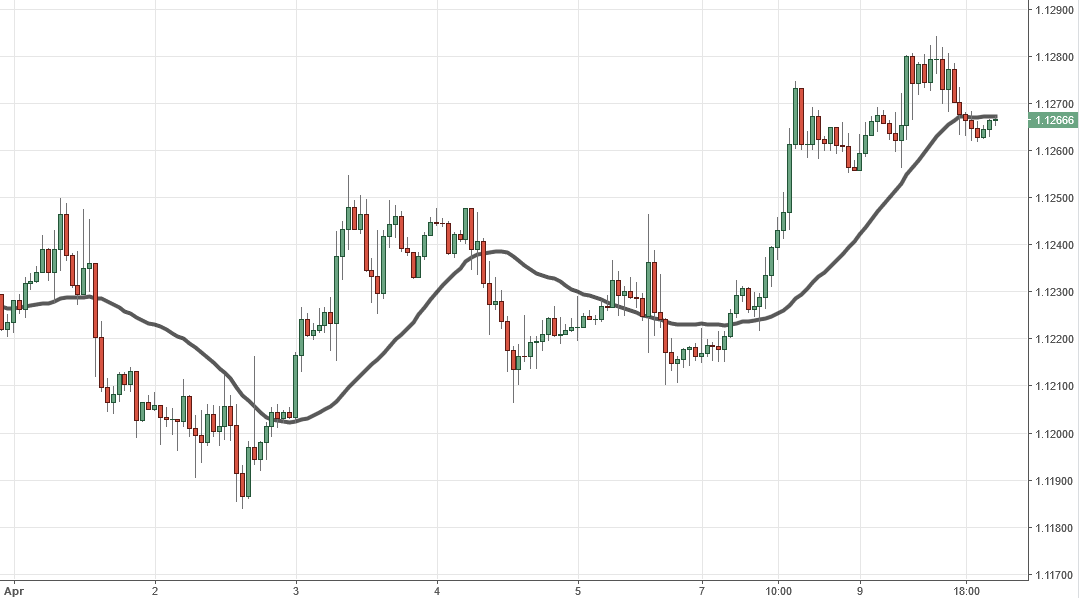
\includegraphics[width=1.0\textwidth]{img/moving-average.png}
  \label{figure:moving-average-example}
\end{figure}

Some researchers believe that technical analysis works because it falls under
the category of a self-fulfilling prophecy \cite{salganik2008leading}: it works
because many people use it. If enough people buy an asset because technical
analysis predicts that it is a good idea to do so, the price will rise and then
technical analysis is correct. Nevertheless, there is a big number of technical
indicators, and many of these technical indicators are parametrized, which means
that there are many possible ways of interpreting a market using technical
indicators. Still, there is enough empirical evidence that demonstrates that
technical analysis can help a trader to better understand a market. A possible
explanation behind this is that, although there are virtually an infinite number
of possible configurations that a technical indicator can adopt, not all of them
seem to "follow the market," i.e. a technical indicator needs to be configured
to match the behavior of past prices, and not simply use an arbitrary
configuration. This further reinforces the self-fulfilling prophecy hypothesis
behind technical analysis: the traders that are creating the price movements in
a market are using technical indicators that are being adjusted to the price
that they created themselves.

Taking into consideration the discussion in the previous paragraph, technical
indicators thus work by trying to find a pattern in the price movements. These
patterns are then interpreted in some way by traders, and inferences about the
market are created, such as: "this market is presenting a high volatility" or
"this market is going uptrend." This also implies that technical indicators can
be interpreted in different ways, depending on the trader's knowledge and
opinion.

In conclusion, in order to understand a market from a technical analysis point
of view, one needs to take into consideration that a number of traders with
different ideas and different interpretations of the market are creating the
price movements. Forecasting or modelling tools taking a technical analysis
approach should take into consideration these factors.

\section{Thesis Structure}
\label{section:thesis-structure}

% Comments are placed after each sentence % consider doing a hard wrap to 80 or
% so characters so.  % This will make easier to place comments on each line, for
% GitHub

The objective of this thesis is to propose a novel series of approaches on how
to analize and interpret a financial market to obtain insights that can be
used to describe the behavior behind that market and create a profitable trading
strategy. In this first Chapter the reader finds the motivation of this work,
such as why understanding a financial market is a problem and why solving this
problem is beneficial (see Section \ref{section:justification}).

% In the first sentence "propose a novel series of approaches to how a financial
% market can be interpreted and analyzed"


% the things you approach "interpreted and analyzed" are to far away, maybe:
% ... approaches on how to analize and interpret a financial market ...  % we
% must try not to use words such as "great importance" change to? " %
% ... solving this problem is beneficial".

The proposed method in this document is based on at least three different
fields, which are computational intelligence, complexity theory and financial
markets. Chapter \ref{chapter:preliminaries} is dedicated to explaining the
concepts related to these fields, which are needed to understand the contents of
the following Chapters and the thesis overall.

% Depending on space the comment on the background of readers could be deleted.

Once the reader is acquainted with the necessary terminology, concepts and ideas
discussed in the aforementioned Chapter, a series of related works is presented
in Chapter \ref{chapter:related-work}. These works help the reader to further
understand the problem being solved in this thesis, as one can see how different
approaches have been taken in the past to solve similar problems. Also, the
presented related works indirectly fuel the justification of this thesis, as the
reader can realize how similar approaches to the proposed method have improved
other fields of research.

The actual proposed method of this thesis is presented in Chapter
\ref{chapter:proposed-method}. In this Chapter the reader can find how the
problem discussed in Section \ref{section:description-of-the-problem} can be
solved. Additionally, some other proposals are discussed, such as how
intuitionistic fuzzy sets and systems can be used to represent a knowledge in an
expanded way, in contrast to traditional fuzzy sets and systems.

A particular implementation of the proposed method is discussed in Chapter
\ref{chapter:implementation}, which covers some technical details, such as what
programming languages were used and how exactly the ideas from Chapter
\ref{chapter:proposed-method} were programmed. As each of the concepts discussed
in Chapter \ref{chapter:proposed-method} are covered in the implementation, some
of the Sections from both Chapters match in name.

After having implemented the proposed method, a series of experiments were
performed to demonstrate how it compares to other similar solutions. The
experiments also help the reader to understand how the method can be used to
obtain insights from a financial market, as well as how one can use these
insights to perform better decisions while trading such markets. These
experiments are presented in Chapter \ref{chapter:experiments}, where their
design is discussed, and the results obtained from the experiments are presented
in Chapter \ref{chapter:results}.

Lastly, the reader can find some conclusions about the work developed for this
thesis in Chapter \ref{chapter:conclusions}, as well as various propositions on
how the present work could be further developed in the future in Chapter
\ref{chapter:future-work}.

\section{Justification}
\label{section:justification}

Understanding the nature of financial markets is of utter importance, as
financial markets play a big role in the economy system of any country. Having
several tools to understand financial markets can help to forecast financial
crises, understand the development of the economy of a company, and take better
decisions when investing.

The problem stated in Section \ref{section:description-of-the-problem} can be
broken into the following pieces: a forecasting or modelling solution needs to
consider 1) a number of traders manipulating the price movement in a financial
market, 2) each of these traders have different opinions about how to trade a
market depending on how the market is behaving, and 3) each of these traders
interpret the market differently.

Traders can be seen as agents in a multi-agent system, where each of these
agents receive data from another agent: a broker. The broker is in charge of
sending the price information about a financial market to every trader. This
data can be used later as the input for all the technical indicators. The agents
representing the traders never interact among them, only with the broker. In
addition to receiving the financial market data from the broker, a trader can
also send transaction operations to the broker, such as buy or sell orders. Many
authors consider multi-agent systems and agent-based models as one of the better
tools for modelling and simulating financial markets \cite{Lebaron2001}
\cite{Gamil2007} \cite{Boer-Sorban2008}, due to their flexibility to represent
very complex systems.

Implementing an agent-based solution allows not only to simulate the actions
that different entities can take in a complex system, but also to model how the
agents are perceiving their environment and the inference process used to take
such actions. This is interesting because the simulated models created using an
agent-based solution can then be examined by looking at how each of the agents
behaves in the system.

%% Then talk about how to model the agents' actions or belfies, etc.

%% We can justify two things: why the problem is important and why the
% method works

%% why multi-agent, why intuitionistic, why retracements

\chapter{Preliminaries}
\label{chapter:preliminaries}

The following Sections describe all the concepts required for the reader to
understand the proposed method in this thesis. However, it is still assumed that
the reader has some basic knowledge about programming and computational
intelligence. For this reason, the following concepts are focused on terms
related to finance, specifically to trading and financial markets, and to
agent-based models and multi-agent systems.

\section{Financial Market}
\label{section:financial-market}

A financial market is constructed by the interaction of a number of traders,
where a trader is an entity that is able to buy or sell a number of units of an
asset \cite{Huang2009}. The entities defined as traders can either be individual
human beings, organizations or even computer programs \cite{Lu2009}. An asset
can be anything that can be priced and can be divided so different parties can
hold a share of the asset \cite{Avramov2006}. For example, corn can be priced
and different parties can hold a share of the corn market by physically owning
corn. Lastly, traders can decide to either buy or sell shares of this
asset. Although this decision can seem simple, as there can only be two
outcomes, the process a trader can follow in order to arrive to an outcome can
be very complex.

In theory, if one can know all the variables that each trader is taking into
consideration to arrive to their particular decisions, the prices in a financial
market can be precisely predicted \cite{Garcia-Almanza2006}. Obviously, this is
impossible, unless we were simulating a financial market with a handful of
people and everyone was telling everyone else what decisions they are going to
take. Nevertheless, one can create models that closely simulate a financial
market, and one can assume that these simulations are generalizations of the
real financial market \cite{Cai2013}.

\section{Trading Strategy}
\label{section:trading-strategy}

A trading strategy is a set of processes that help a trader to determine
different aspects of a financial market and to later make trading decisions
based on these aspects \cite{Kendall2003}. For example, a trader can determine
that a market is going to follow an uptrend -- that is, that the price of a
financial market is going to rise -- and take the decision of buying shares of
the asset of that financial market. Trading strategies can vary in complexity:
some can use simple moving averages to determine trends and entry points, and
others can take into consideration many different indicators, as well as the
trader's experience.

An untrained person can think that trading a financial market only involves
deciding when to buy or sell a market. Nevertheless, the possible decisions can
be as complex as the strategy used to determine them. For instance, when traders
are about to open a new buy or sell order, they also need to decide the size of
the order, or how many units are going to be bought or sold. These units can be
shares in a stock market or an amount of a currency in foreign exchange markets,
for example. This order can also be delayed: the trader can decide that an order
will be opened when a certain amount of time passes or when certain price in a
financial market is reached. Additionally, the trader can specify \textit{stop
  loss} and/or \text{take profit} prices: after executing a buy or sell order,
if the market reaches certain price, the trade has to be cancelled, stopping any
losses or taking any profits that that trade generated since it was created.

The initial process of creating a trade order is complex, as noted in the
previous paragraph, but decisions can also take place after a number of trade
orders have been executed. The most obvious decision is when one should stop a
trade. This particular decision has spawned several psychological research
works, where the decision process is analyzed \cite{Maranon2018}. A clear
example is depicted in Figure \ref{figure:trading-psychology}, where the
emotions that traders generally feel when experiencing the earnings or losses of
a trade are shown (extracted from the work by Baker and Riciardi \cite{BakerHKentandRicciardi2014}).

\begin{figure}
\centering
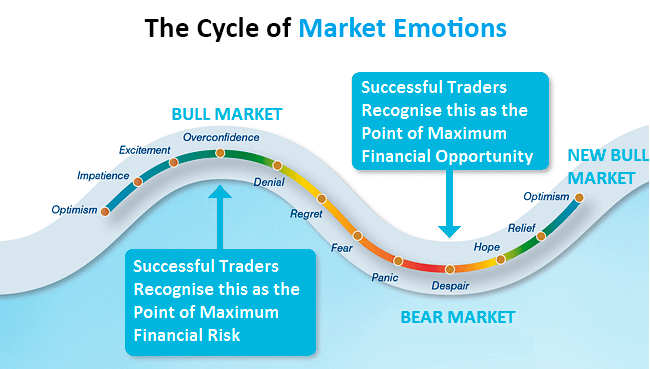
\includegraphics[width=1.0\textwidth]{img/trading-psychology.png}
\caption{Investor sentiment and the business cycle}
\label{figure:trading-psychology}
\end{figure}

Stopping a trade does not only involve emotions, as a thorough analysis of the
market, about the current's account financial situation and the trades
themselves needs to be performed \cite{Kadiri2015}. Regarding about the first
step -- an analysis of the market -- it is worth mentioning that these analyses
are usually different than those performed when deciding when to start trading a
market \cite{Conrad1998} \cite{Muller1997}. For example, in a stagnated market
one could decide not to trade a market, but this does not necessarily mean that
one should close trade orders in this situation; one could consider that this is
a moment where trades need to be held until further price movements take
place. A trader can also decide to \textit{partially} stop a trade; that is, a
trader can decide to sell a certain amount of units from a trade, for
example. Likewise, a trader can decide to acquire more units from the asset.

It is usual that a trader \textit{diversifies} its trading portfolio
\cite{Muller1997}. Diversifying means that a trader starts trading a number of
financial markets instead of focusing on a single market. The advantages of this
are that the risk diminishes, as the profits of trading some markets can
compensate the losses obtained from trading other markets
\cite{Muller1997}. Diversification can then make trading strategies even more
complex, as a trader now needs to take into consideration different
markets. Additionally, markets usually affect the price movements of other
markets, for example, if wheat price goes up, this can directly impact the price
of McDonald's stock prices, as many of their products contain wheat-based
ingredients. Furthermore, if McDonald's stock market is severely affected, this
could negatively impact the United States' economy, as McDonald's is one of the
most profitable companies in this country. Depending on the robustness of a
trading strategy, all of these aspects can be considered to take a decision.

Trading strategies have existed since the activity of trading was created.  To
illustrate this, one can consider how the Japanese traded certain commodity
markets, such as the rice market, using strategies based on candlestick patterns
\cite{Nison1991}. The Japanese charted the prices by representing the open,
highest, lowest and close prices for a period of time using figures that
resemble candles and their wicks, as the those seen in Figure
\ref{figure:candlestick-chart}. The body of a candle in this type of charts
represents the opening and the closing prices of a session, while the wick
represents the lowest and highest prices that occurred during the session.

%% These two will be redesigned to match the thesis document style
\begin{figure}
\centering
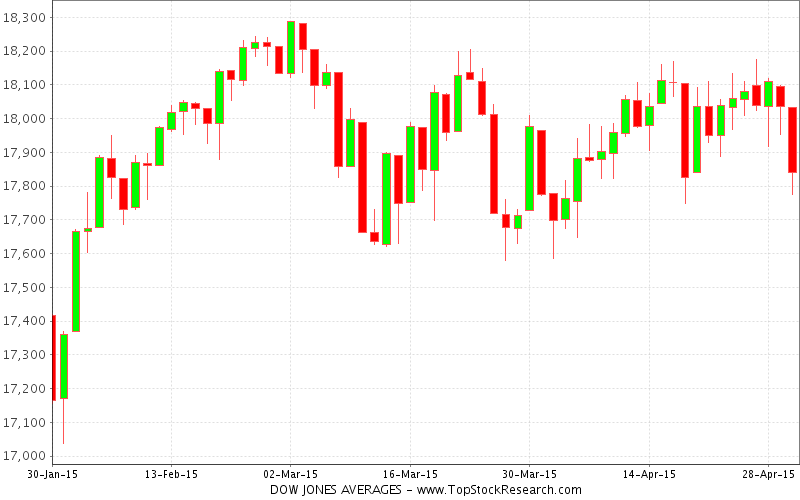
\includegraphics[width=1.0\textwidth]{img/candlestick-chart.png}
\caption{Example of a candlestick chart}
\label{figure:candlestick-chart}
\end{figure}

Japanese traders noticed patterns that emerged in the candlestick charts. These
patterns helped the traders to understand the current situation of a financial
market and to take decisions based on these assumptions. Some example patterns
are shown in Figure \ref{figure:candlestick-patterns}. For example, if a
``bullish engulfing'' or a ``rising sun'' candlestick pattern appears in the chart
of a market, this is considered as a sign of a following uptrend -- which means
that prices will increase. In contrast, if a ``bearish engulfing'' or ``dark cloud
cover'' candlestick pattern appears, this signs a following downtrend -- which
means that prices will decrease. Additionally, there are patterns that indicate
that a market will start stagnating, such as the ``harami'' candlestick
pattern. It is worth noting that these candlestick patterns are still used in
modern trading strategies \cite{Nison1991}.

All the processes described above can be performed manually, i.e. a trader can
look at price charts and start identifying candlestick patterns, draw moving
averages over the chart, decide on the number of units to buy or sell, decide on
take profit and stop loss levels, etc. However, with the introduction of
computers to the financial world in the mid 20th century, automated or
algorithmic trading was also introduced \cite{Hendershott2011}. Algorithmic
trading help traders to partially or totally delegate trading tasks to computer
software, where buy or sell transactions occur when a set of conditions are
met. In this thesis, an automated trading strategy is part of the proposed
method.

\begin{figure}
\centering
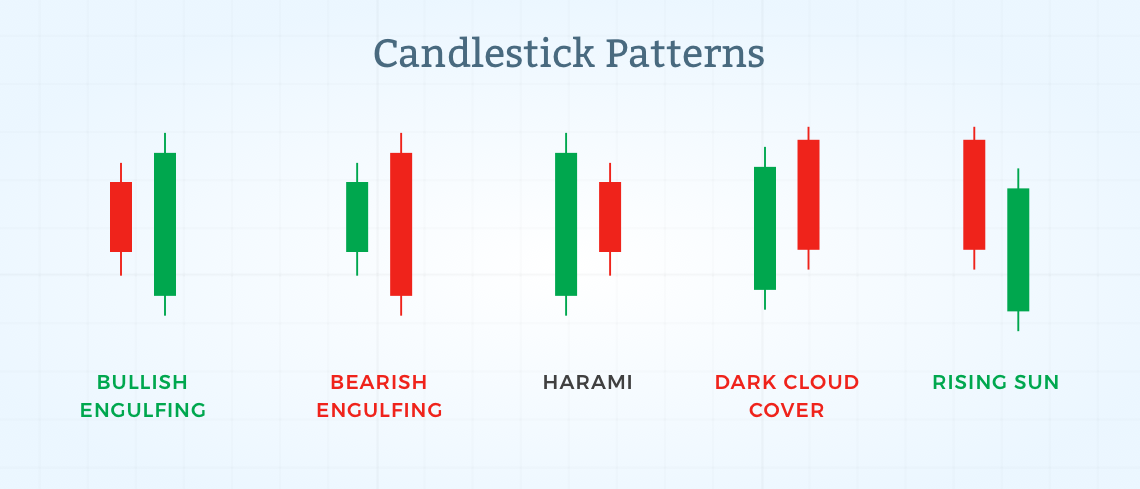
\includegraphics[width=1.0\textwidth]{img/candlestick-patterns.png}
\caption{Examples of candlestick patterns: (a) bullish engulfing, (b) bearish engulfing, (c) harami, (d) dark cloud cover, (e) rising sun}
\label{figure:candlestick-patterns}
\end{figure}

\section{Technical Analysis}
\label{section:technical-analysis}

Since many decades ago, financial traders have implemented statistical models to
forecast time-series, as part of a field called technical analysis
\cite{Lo2000}. This type of market analysis is characterized by using past
financial data to describe certain aspects of a market, such as its volatility,
trend, and momentum \cite{Achelis2000}. These indicators receive the name of
technical indicators. Some examples of technical indicators are those created by
Welles Wilder, such as the Relative Strength Index (RSI) and the Average
Directional Index \cite{Wilder1978}, and an example of an oscillator, which is a
type of technical indicator which usually tells if a market is overbought or
oversold, is the Stochastic Oscillator \cite{Schirding1984}, created by George
Lane. In contrast to technical analysis, fundamental analysis relies on the
examination of the underlying forces that affect a particular financial market
(or several of them), instead of just relying on the price movements in a
time-series. As an example of fundamental analysis, a trader can use the
financial statements of a public company to estimate if the price of their stock
will rise.

A more modern approach to perform these analyses is to use machine learning
techniques. Using machine learning algorithms, researchers create regression
models using technical or fundamental indicators as training datasets
\cite{Connor2005}.  Examples of regression techniques are autoregression
\cite{burg1968new}, symbolic regression \cite{billard2002symbolic}, and linear
regression \cite{kutner2004applied}. Other more elaborated techniques exist in
machine learning for regression or curve-fitting tasks, such as the use of
artificial neural networks \cite{melin2007hybrid} and support vector regression
\cite{basak2007support}.

\subsection{Retracements in Financial Markets}
\label{subsection:retracements-in-financial-markets}

A retracement in a financial market is any market price movement that goes
against a clear trend in a determined timeframe, but where the magnitude is not
significant enough to point to a reversal in the market's direction. For
example, if a stock market has been going upwards in price for the past three
months, and in the past week the price went downwards, this movement could be
considered a retracement. The retracement movement is confirmed once the market
retakes the general price direction. If the market never retakes this general
direction, a reversal is said to have occurred. An example of retracements in a
financial market price chart can be seen in Figure
\ref{figure:retracements-in-financial-market}.

\begin{figure}
\centering
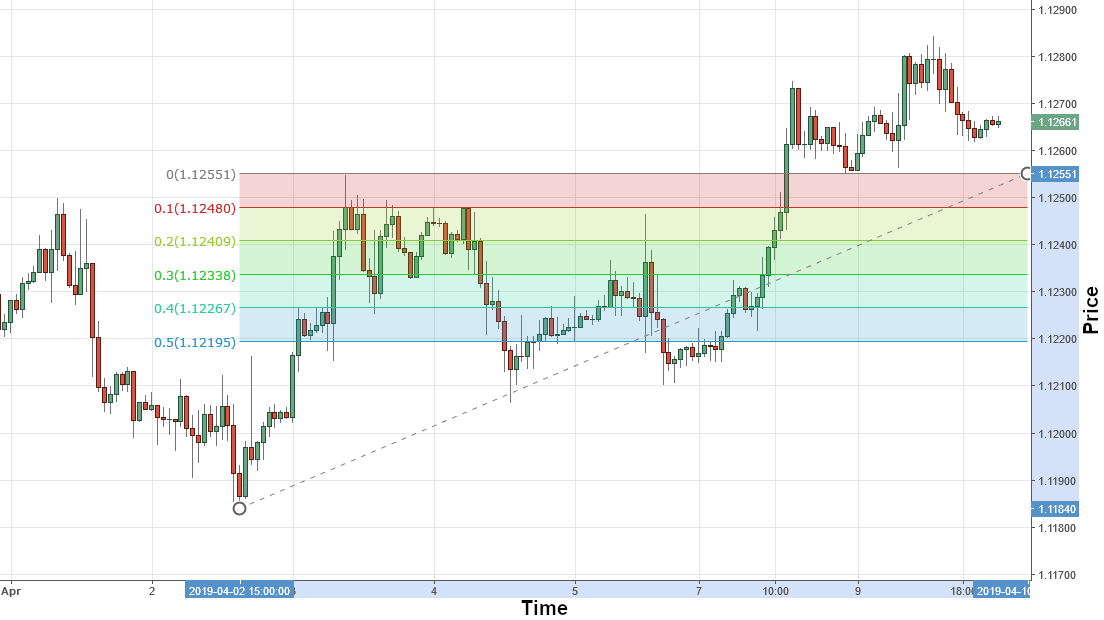
\includegraphics[width=1.0\textwidth]{img/retracements.png}
\caption{Example of retracements in a financial market price chart}
\label{figure:retracements-in-financial-market}
\end{figure}

A special type of retracements are Fibonacci retracements. In this type of
retracements, the market usually follow retracement movements that correspond to
Fibonacci ratios. For example, if a market has been following an uptrend in its
prices for the past 1000 units, and the market suffers a retracement of
approximately 382 units, it is said to be a Fibonacci retracement, as this
retracement follows a ratio of 0.382. Fibonacci retracements commonly occur
in financial market price charts. An example of fibonacci retracements can be
seen in Figure \ref{figure:fibonacci-retracements-in-financial-market}. It is
worth to mention that retracements do not always occur and they do not follow
the ratios exactly.

% Seems like ``retracements'' are heuristics. You should make this clear, we
% do not want the readers to think they are proven facts, or worst, that
% they think we are treating them as if they where. 

\begin{figure}
\centering
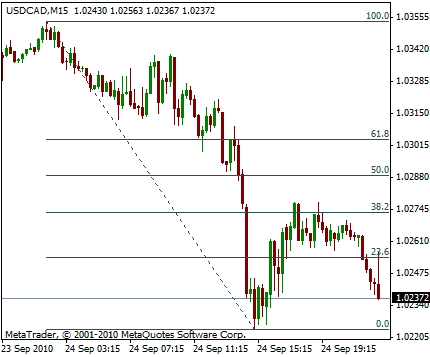
\includegraphics[width=1.0\textwidth]{img/fibonacci-retracements.png}
\caption{Example of Fibonacci retracements in a financial market price chart}
\label{figure:fibonacci-retracements-in-financial-market}
\end{figure}

\section{Computational Intelligence}
\label{section:computational-intelligence}

Computational intelligence is a field of computer science similar to artificial
intelligence. In contrast to artificial intelligence, where symbolic logic is
used to represent reasoning, computational intelligence relies on statistical
and bio-inspired approaches
\cite{JangJyh-ShingRogerandSunChuen-TsaiandMizutaniEijiandHo1998}. As the models
generated by computational intelligence are often not exact, but rather an
approximation to the problem it is modelling, it is sometimes also called soft
computing.

The following Sections discuss the computational intelligence techniques that
are used in the proposed method of this thesis.

\subsection{Fuzzy Sets}
\label{subsection:fuzzy-sets}

A traditional set is a collection of items that share a common
characteristic. This characteristic serves as a membership, because all the
items in a universe either have that characteristic -- and then the item is part
of the set -- or it does not have it -- and then the item is not part of the
set. Traditional sets can be extended to fuzzy sets, as explained by Zadeh
\cite{Zadeh1965}. Fuzzy sets are then a generalization of traditional sets,
i.e. any traditional set can be represented as a fuzzy set. The difference
between these two types of sets lies in the concept of membership: memberships
are not only used to represent binary outcomes, i.e. \textit{true} or
\textit{false}, but a possibly infinite number of outcomes. An item can now be
partially a member of a set, and the only way an item is not part of such set is
if its membership is totally \textit{false}. In order to represent this grade of
membership one can use real numbers. Thus, one can say, for example, that an
item is \textit{0.7 green}, \textit{0.5 blue} and \textit{0.0 red}. These values
can represent an adverb and an adjective, such as ``very green,'' ``somewhat blue''
and ``not red at all.'' This is especially useful when designing fuzzy systems
(see Subsection \ref{subsection:fuzzy-systems}).


\subsection{Fuzzy Systems}
\label{subsection:fuzzy-systems}

In traditional logic one can generate logical inferences, such as \textit{if
  it's raining, then there are clouds in the sky}. In a similar fashion, one can
use fuzzy sets to represent the antecedents and consequents in a logical
inference process. For example, one can extend the previous example to:
\textit{if it's raining a lot, then there are many clouds in the sky}.

There is a number of ways in which one can construct a fuzzy inference system,
where one or more inputs or antecedents can be used to generate one or more
outputs or consequents. Arguably, the two most popular types of fuzzy inference
systems are the ones created by Mamdani and Assilian \cite{Mamdani1975}, and
Takagi and Sugeno \cite{Takagi1985}. These systems use a series of fuzzy sets to
represent the relationship between an input and its grade of membership to a
set. These sets usually represent adjectives that describe the inputs, and are
also considered to be the antecedents in the fuzzy inference system. For
example, an input of 0.8 can represent a ``very high'' value. After obtaining
these grades of membership, one can use these values to ``fire'' or ``activate'' the
consequents. In the case of a Mamdani system, the consequents are represented as
fuzzy sets, just like the antecedents. In contrast, in a Sugeno system,
consequents are represented by mathematical functions. A set of rules is used to
determine the relationship between the antecedents and the consequents, for
example: \textit{if food quality is high then tip is high}. The aforementioned
rule is creating a relationship between the fuzzy set that represents ``high food
quality'' in the antecedents, and the fuzzy set that represents ``high tip'' in the
consequents. Further continuing with the example, if ``food quality'' is
represented by a value of 0.8, the rule that creates the relationship between
``food quality'' and ``tip'' could determine a ``tip'' of 0.8 too, depending on what
membership function and what parameters are decided to be used to represent
each.

It has been explained how a relationship between antecedents and consequents can
be constructed in a fuzzy inference system. Nevertheless, the most interesting
problem arises when a problem involves several fuzzy sets to represent different
adjectives for single antecedents or consequents. In these cases, depending on
the fuzzy rules, a number of consequents can be fired according to the inputs to
the system. As seen in Figure \ref{figure:antecedents}, the input -- represented
by the dotted vertical black line -- is associated with three fuzzy triangular
sets or antecedents, where it ``activates'' two of them. According to a set of
fuzzy rules, it then fires a set of triangular fuzzy sets that represent the
consequents, as seen in Figure \ref{figure:consequents}.

The fuzzy sets that represent the consequents are cut, and new shapes are
obtained using those cuts, as represented by the green shapes in Figure
\ref{figure:consequents}. These shapes are aggregated and result in the output
of the fuzzy inference system, and this result can then be defuzzified
(converted from a fuzzy set to a scalar or crisp value) using different methods,
such as obtaining the centroid of the shape. In this example, a Mamdani fuzzy
inference system is considered; in the case of a Sugeno system, for example, the
antecedents would be represented by arbitrary mathematical functions, instead of
membership functions representing shapes such as the triangles in the example
presented above.

\begin{figure}
\centering
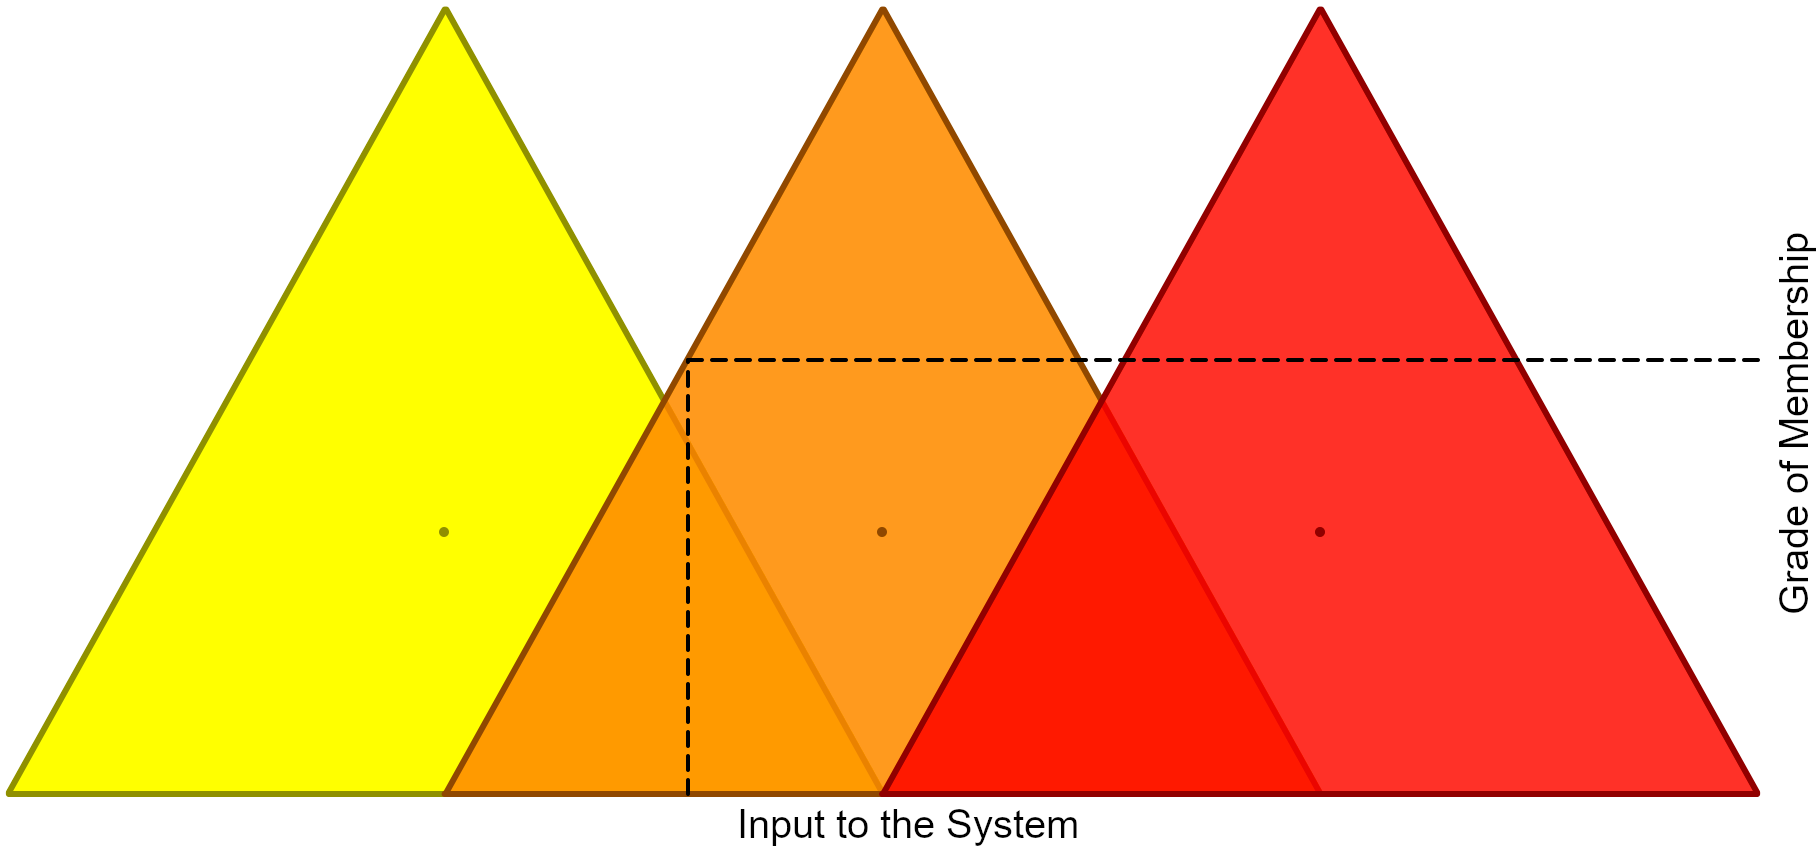
\includegraphics[width=1.0\textwidth]{img/antecedents.png}
\caption{Antecedents in a fuzzy system}
\label{figure:antecedents}
\end{figure}

\begin{figure}
\centering
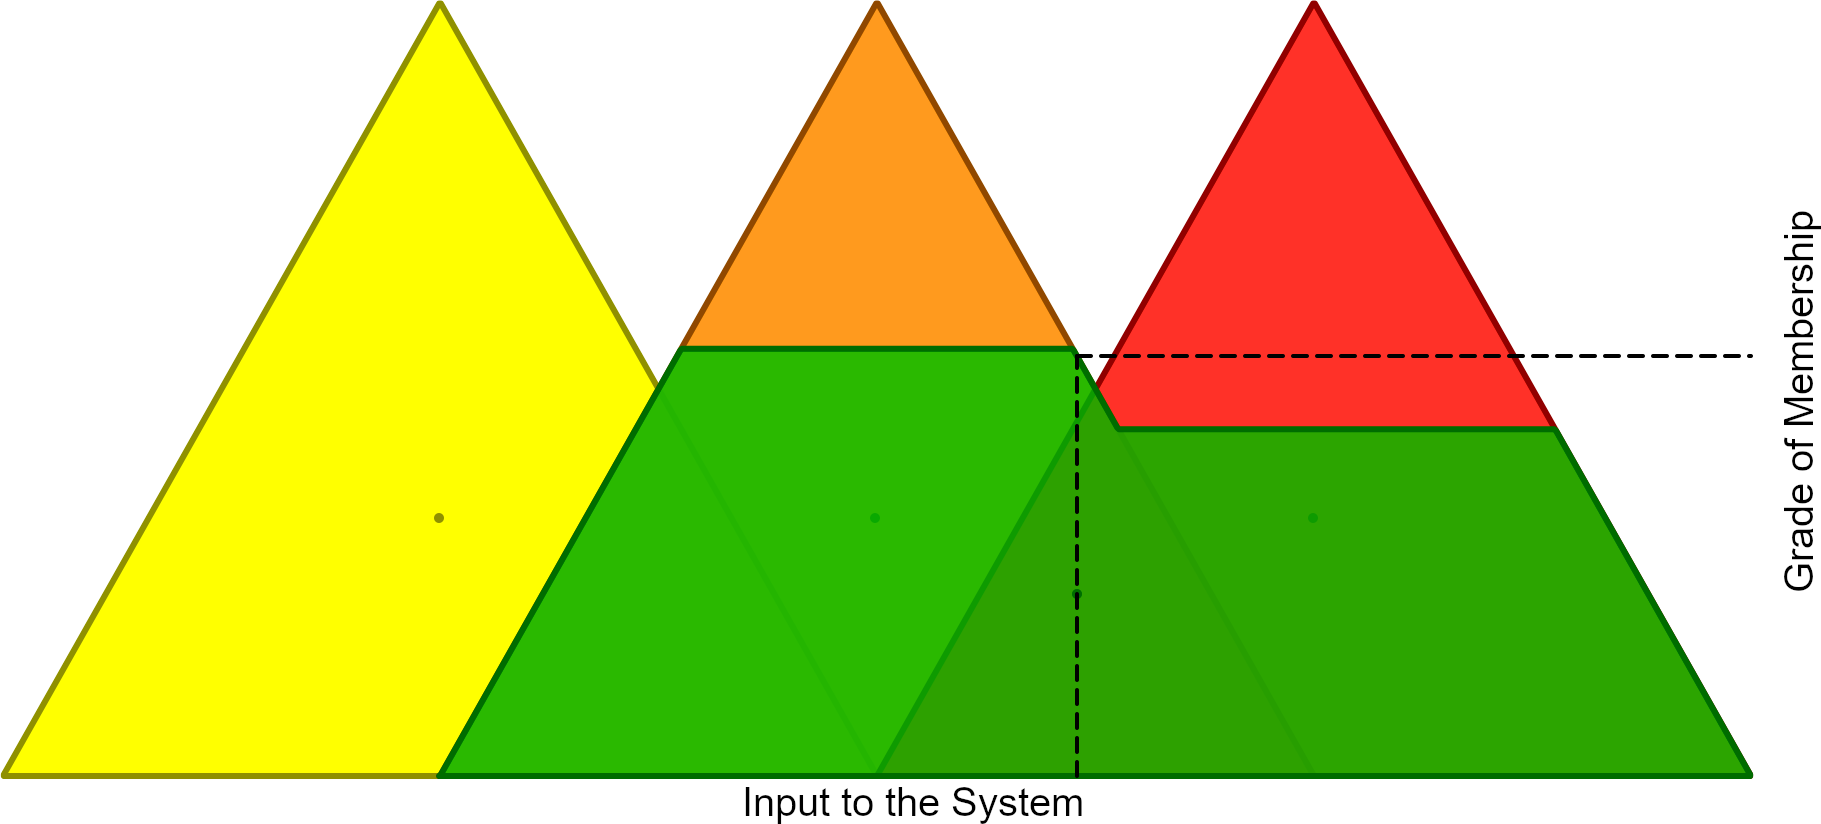
\includegraphics[width=1.0\textwidth]{img/consequents.png}
\caption{Consequents in a fuzzy system}
\label{figure:consequents}
\end{figure}

\subsection{Fuzzy Systems Software}
\label{subsection:fuzzy-systems-software}

There are a number of implementations of fuzzy systems toolboxes or libraries
where a programmer can design a fuzzy system to be integrated with other
software projects or used as stand-alone applications. The vast majority of this
software is dedicated to the creation of type-1 fuzzy systems, i.e. systems that
do not consider uncertainty in the grade of membership of their antecedents or
consequents.

Wagner presents a robust implementation of FISs developed in Java in
\cite{Wagner2013}. Although the toolkit does not provide many tools
for representing a FIS graphically or for interacting with one, the
implementation provides libraries for building type-1, interval type-2, and
generalized type-2 fuzzy systems.

Moreover, the work by Castro et al. \cite{castro2007interval} provides the same
capabilities as the work by Wagner, but in this case it is an implementation in
Matlab. A direct disadvantage of using this programming language is that Matlab
is not a free nor open source software.  Nevertheless, the language is still
widely used in the scientific community. Furthermore, this implementation
follows an interface similar to the one provided by Matlab's fuzzy logic
toolbox, and provides more robust graphical implementations than the current
version of Wagner's toolkit.

For this this thesis a fuzzy system was created from scratch. This decision was taken because it would facilitate its integration with the multi-agent system that was also implemented from scratch and because the author of the proposed method could not find any implementation of a Mamdani intuitionistic fuzzy system at the time when the implementation of the system started. This implementation is described in \cite{Hernandez-aguila2016} and \cite{Hernandez-Aguila2017}.

\subsection{Intuitionistic Fuzzy Sets}
\label{subsection:intuitionistic-fuzzy-sets}

In contrast to the traditional fuzzy sets discussed in Subsection
\ref{subsection:fuzzy-sets}, intuitionistic fuzzy sets consider a grade of
non-membership in addition to a grade of membership associated to an element in
the fuzzy set, as expressed by Equation \ref{eq:ifs-definition}. Intuitionistic fuzzy
sets were defined by Atanassov in \cite{Atanassov1986}.

% intuitionistic fuzzy set
\begin{equation}
  \label{eq:ifs-definition}
  A^{*} = \{\langle x, \mu _{A} (x), \nu _{A} (x) \rangle | x \in E\}
\end{equation}

For every of the elements contained in an intuitionistic fuzzy set,
Equation \ref{eq:intuitionistic-interval} must hold true.

% intuitionistic interval
\begin{equation}
  \label{eq:intuitionistic-interval}
  0 \leq \mu_{A}(x) + \nu_{A}(x) \leq 1
\end{equation}

Intuitionistic fuzzy sets are an extension to traditional fuzzy sets, as any
traditional fuzzy set can be expressed as a particular case of an intuitionistic
fuzzy set, as in Equation \ref{eq:ifs-form}.

% every ordinary fuzzy set has the form
\begin{equation}
  \label{eq:ifs-form}
  \{ \langle x, \mu_{A}(x), 1 - \mu_{A}(x) \rangle | x \in E \}
\end{equation}

If the sum of the membership $\mu_{A}(x)$ and non-membership $\nu_{A}(x)$ of an
element is less than $1$, the concept of indeterminacy or hesitancy arises,
which is described by Equation \ref{eq:indeterminacy}. Indeterminacy is used to represent
doubt in the grade of membership of an element in an intuitionistic fuzzy set
and is described by Equation \ref{eq:indeterminacy}.

% if
\begin{equation}
  \label{eq:indeterminacy}
  \pi_{A}(x) = 1 - \mu_{A}(x) - \nu_{A}(x)
\end{equation}

Traditional fuzzy sets can be extended to increase their capabilities of
representing uncertainty by introducing the concept of footprint of
uncertainty. A footprint of uncertainty is achieved by extending the membership
function, where each of its values are now fuzzy sets themselves, instead of
crisp values. This type of traditional fuzzy sets are commonly labeled as type-2
fuzzy sets in the literature \cite{Mendel2006}.

Indeterminacy serves a different purpose than the one of footprint of
uncertainty. Instead of extending the uncertainty provided by traditional fuzzy
sets, indeterminacy helps to model doubt \cite{Xu2007}. For example, if
traditional fuzzy sets can model the following sentence: ``the object is very
hot'', indeterminacy can model ``it is unsure that the object is very hot''.

\subsection{Intuitionistic Fuzzy Systems}
\label{subsection:intuitionistic-fuzzy-systems}

Human beings tend to express their knowledge using natural language and certain
words to describe abstract objects or experiences in fuzzy terms. For example,
after generating a financial report, one is interested in knowing if an
organization is ``doing well,'' or if it is ``not profitable enough.'' The
previous examples are fuzzy statements that need to be inferred from data, but
this data can also be uncertain (e.g. noise is present in the data). For that
reason, fuzzy sets have been proposed for data modeling and knowledge
representation. On the other hand, fuzzy inference systems (FIS) have been
applied in the construction of control and pattern recognition systems also
based on such fuzzy data. Nevertheless, occasionally there are situations where
a traditional FIS can not properly model certain data sets, due to high levels
of uncertainty present in the data (e.g., noise). As a consequence, researchers
have extended fuzzy sets and fuzzy logic theory to allow the construction of
systems that can successfully represent noisy data.

One of the extensions to fuzzy sets are type-2 fuzzy sets \cite{Mendel2002}. The
idea behind this extension is to add uncertainty to the membership of an element
to a fuzzy set. In other words, an element will have a grade of membership to a
fuzzy set, and this grade of membership will be represented as another fuzzy
set. For example, this technique allows a fuzzy system to be more resilient to
data with many outliers; it will be easier for a type-2 fuzzy system to create a
generalized model of the data than a type-1 fuzzy system. Many works have
incorporated type-2 fuzzy sets into their systems and have obtained better
performance when compared to their traditional or type-1 fuzzy sets counterparts
\cite{Liang2000}. Despite this increase in capabilities for handling
uncertainty, type-2 fuzzy systems have the disadvantage of being significantly
slower than type-1 systems \cite{Sepulveda2012}. The reason for this penalty in
performance is mainly due to how a type-2 fuzzy system is implemented, that is,
the programming language used for it and what type of programming techniques
were used to implement the fuzzy theory. One way to mitigate this problem is to
restrict the fuzzy sets that represent the grade of membership for an element,
in order to simplify the calculations needed for the system to generate
inferences, and therefore quicken the process. Interval type-2 fuzzy systems
were the result of implementing this idea, which are a particular case of
general type-2 fuzzy systems \cite{Mendel2006}. Another way is to reduce the
complexity of the algorithm, such as in the case of the work from Karnik and
Mendel \cite{Karnik2001}.

Fuzzy sets can also be extended to intuitionistic fuzzy sets (IFS), which are
proposed by Atanassov in \cite{Atanassov1986}. As in the case of type-2 fuzzy
sets, IFS increase the capabilities of a traditional fuzzy set to represent
uncertainty, by introducing the concept of indeterminacy. Basically an element
that belongs to an IFS is described by a grade of membership (\(\mu\)) and a
grade of non-membership (\(\nu\)). One can express how well an element belongs
to a fuzzy set and how well an element does not belong to that fuzzy set as
well. As a consequence, the sum of the values for the membership and
non-membership are not always equal to 1, and \(1-(\mu + \nu)\) will be known as
indeterminacy, which is represented by the symbol \(\pi\). FISs that implement
intuitionistic fuzzy sets have at least two advantages: 1) they can handle more
uncertainty than traditional FISs and can process their inferences to crisp
values with almost no resource performance impact, and 2) they can still be
extended to use type-2 fuzzy sets, giving as a result an intuitionistic type-2
FIS.

The use of IFSs in a traditional FIS should enable the handling of more
uncertainty, and one could prefer an intuitionistic FIS (IFIS) to obtain better
accuracies without sacrificing time performance, as inferences in a type-2 FIS
(T2-FIS) are very time consuming compared to a type-1 FIS (T1-FIS). This is a
consequence of the complex type reducing procedure that is involved in the
defuzzification stage in a T2-FIS \cite{Liang2000}. Several improvements to the
algorithms involved in the inference process in a T2-FIS have been proposed to
alleviate this problem, such as the Karnik-Mendel algorithm \cite{Karnik2001}
and shadowed sets \cite{Pedrycz1998}. Nevertheless, a T2-FIS is usually several
times slower than a T1-FIS. Because of this time performance impact, many works
that require handling more uncertainty than a T1-FIS use a particular case of
T2-FIS, the interval T2-FIS (IT2-FIS) \cite{Liang2000}, which is faster than a
general T2-FIS (GT2-FIS). A type-1 IFIS (T1-IFIS) should perform better than a
T1-FIS in terms of accuracy (in problems involving data with high levels of
uncertainty), and should be faster than a T2-FIS. Furthermore, IFSs can be
implemented as part of a T2-FIS, giving as a result a type-2 IFIS.

\subsection{Membership and Non-Membership Functions Design}
\label{subsection:membership-and-non-membership-functions-design}

At the time of writing this thesis, there are not many works involving Mamdani
type intuitionistic inference systems yet, and the author of this work is only
aware of the work by O. Castillo et al. \cite{castillo2007intuitionistic}, and
A. Hernandez-Aguila and M. Garcia-Valdez \cite{Hernandez-aguila2016}. As a
consequence of this lack of works involving Mamdani FISs, there is not a common
way to graphically represent an IFS for its use as membership and non-membership
functions for an IFIS. Additionally, there is not a common way to graphically
represent the architecture of an IFIS.

In this thesis we use the method to graphically represent IFISs' architectures
proposed in \cite{Hernandez-aguila2017-2} in which the author of this thesis
participated. Figure \ref{figure:ifs-proposed} depicts an example of an IFS that
uses the graphical representation proposed in the aforementioned work, and
Figure \ref{figure:ifs-proposed-diff-mu-sd} shows a similar IFS where the mean
of the non-membership function is different than the mean of the membership
function. Also, it is noteworthy how the membership function has core in 0.7 --
instead of 1, as in traditional fuzzy sets -- and the non-membership function
has a core in 0.3.

\begin{figure}
\centering
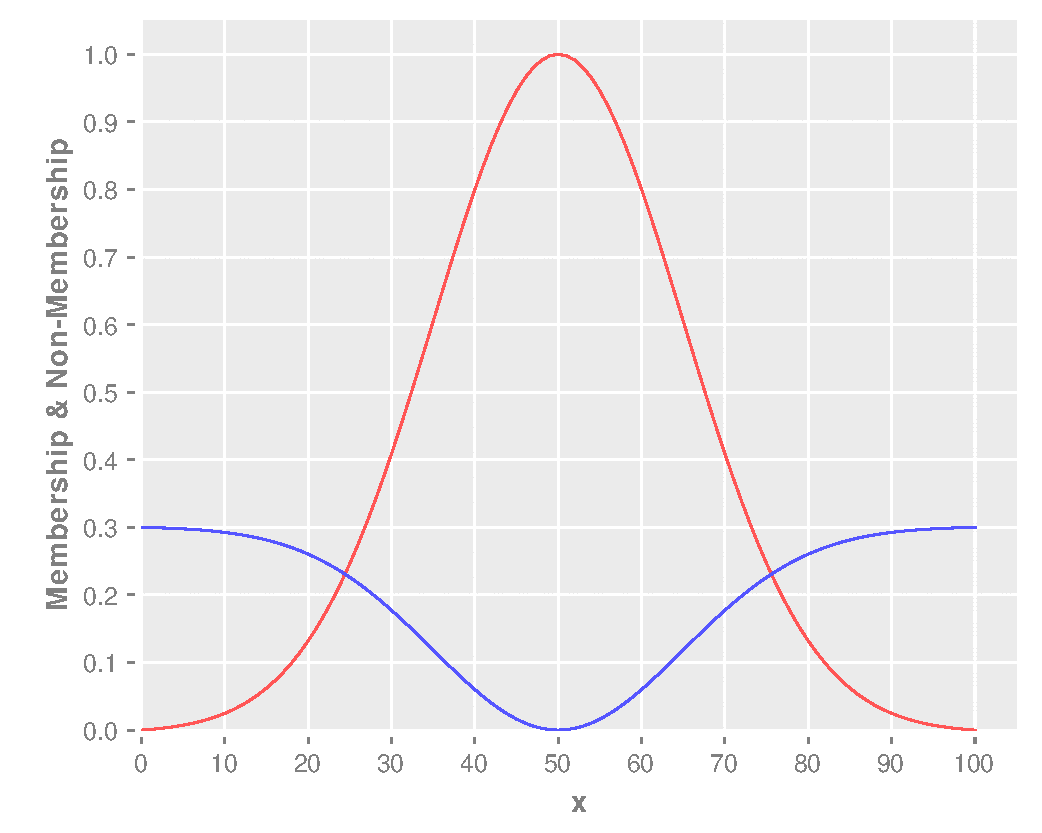
\includegraphics[width=0.7\textwidth]{img/ifs.pdf}
\caption{Example of an intuitionistic fuzzy set with the proposed graphical
  representation}
\label{figure:ifs-proposed}
\end{figure}

\begin{figure}
\centering
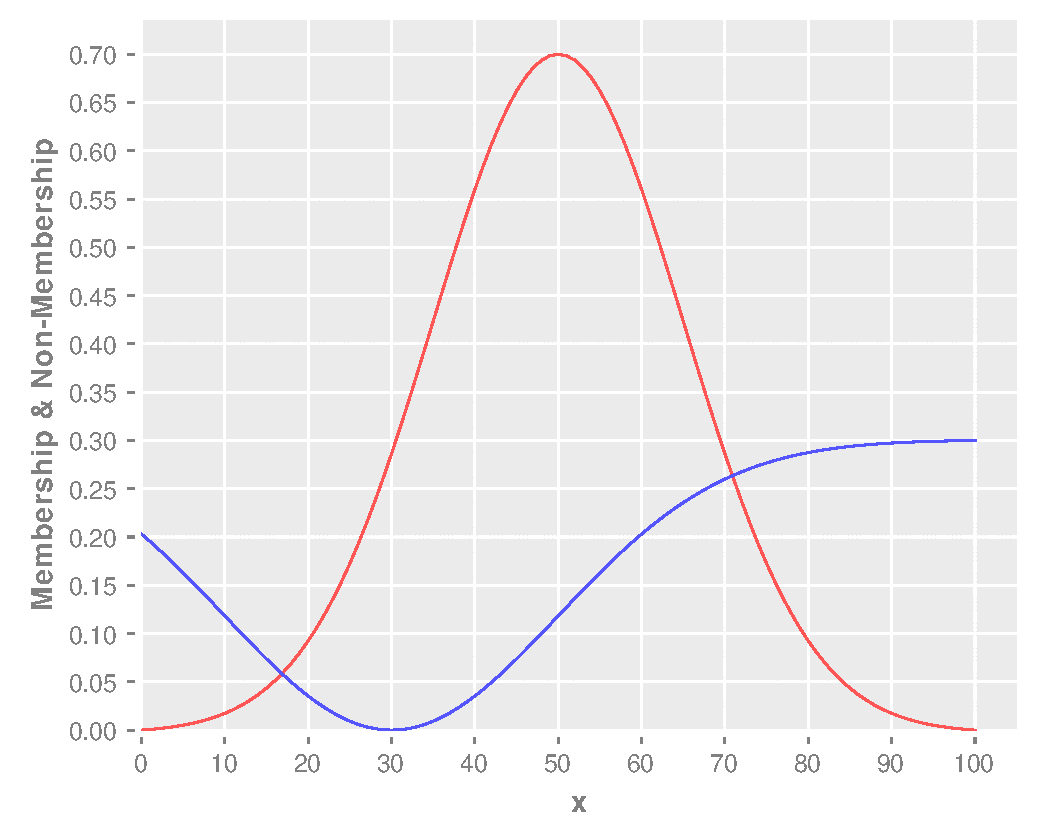
\includegraphics[width=0.7\textwidth]{img/ifs-diff-mu-sd.pdf}
\caption{Example of an intuitionistic fuzzy set with the proposed graphical
  representation with different mean and indeterminacy}
\label{figure:ifs-proposed-diff-mu-sd}
\end{figure}

\section{Genetic Algorithms}
\label{section:genetic-algorithms}

A genetic algorithm (GA) is an optimization algorithm inspired in evolution. For
this reason GAs are considered to be part of a subfield of optimization
algorithms called evolutionary algorithms \cite{Whitley1994}. A GA proposes an
initial set of possible solutions to a problem -- usually called a
population. Each solution in this population is called a chromosome and
sometimes they are referred as individuals. The population is evaluated against
a fitness function, which is going to determine each of the individuals'
performance when trying to solve a particular problem. This problem commonly
involves finding sets of parameters that will cause a system to minimize or
maximize an error.

The population in a GA undergoes an evolutionary process that involves the
crossover among the fittest individuals in the population, and the elimination
of those individuals that perform the worst according to the fitness
function. The crossover process is usually performed by recombining the genes in
the chromosomes of the selected individuals -- which are usually the
fittest. The aforementioned process is usually repeated for a number of
iterations, which are commonly called generations.

In GAs and other evolutionary algorithms, the population will usually start to
become more fit to solve a problem after a series of generations, but it is
common that none of the individuals finds the best possible solution for the
problem. Furthermore, running an evolutionary algorithm several times will most
likely yield different results, as the initial population of solutions are
randomly generated. For this reason, evolutionary algorithms are said to be
meta-heuristic search algorithms, as they find suboptimal solutions to other
problems that do not directly involve the evolutionary algorithm, and they are
also considered stochastic algorithms \cite{Harik1999}.

\section{Multi-agent Systems and Models}
\label{section:multi-agent-systems-and-models}

A multi-agent system is software that solves a problem using agents. Agents can
be seen themselves as programs that interact with their environment, which may
include other agents. Agents in the proposed method in this paper follow the
structure suggested by Shoham in \cite{Shoham1993}, where agents have beliefs
and rules. Beliefs are used by agents to arrive to an interpretation of their
environment, and rules are used to arrive to actions to be performed by the
agent towards their environment. The agents in the system are constantly sensing
their environment to determine what actions to take according to their beliefs
and rules. Multi-agent systems have the objective of solving a practical
problem, unlike agent-based models which are more focused to providing a
simulation of a problem.

As mentioned before, agents can also be used to create agent-based models. These
models are used to represent a problem so a human being can analyze it and infer
new knowledge from it, or it can be used to better understand a problem.

The proposed method in this paper is both a multi-agent system and an
agent-based model. It is a multi-agent system in the sense that it can be used
to create a trading strategy, and it is an agent-based model because the agents
in the system can be analyzed to understand the state of the market that is
serving as the system's environment.

\chapter{Related Work}
\label{chapter:related-work}

\section{Fuzzy Systems in Financial Market Prediction}
\label{section:fuzzy-systems-in-financial-market-prediction}

\section{Type-2 Fuzzy Sets}
\label{section:type-2-fuzzy-sets:related}

\section{Type-2 Fuzzy Systems}
\label{section:type-2-fuzzy-systems:related}

\section{Intuitionistic Fuzzy Systems}
\label{section:intuitionistic-fuzzy-systems:related}

\begin{itemize}
\item At the time of writing, the authors could not find IFIS used in this
\end{itemize}

\section{Multi-agent Systems and Models}
\label{section:multi-agent-systems-and-models:related}

\subsection{Multi-agent Systems and Models in Finance}
\label{subsection:multi-agent-systems-and-models-in-finance:related}

\section{Prediction Models based on Technical Analysis}
\label{section:prediction-models-based-on-technical-analysis}

\section{Retracements in Financial Markets}
\label{section:retracements-in-financial-markets:related}

\section{Elliot Wave Principle}
\label{section:elliot-wave-principle:related}

\section{Regression}
\label{section:regression:related}

\section{Decision Support Systems}
\label{section:decision-support-systems:related}
\chapter{Proposed Method}
\label{chapter:proposed-method}

This Chapter describes each of the modules that integrate the method used to
create the trading strategy proposed in this work and how their integration is
performed.

\section{Preprocessing a Financial Market using Retracements}
\label{section:preprocessing-a-financial-market-using-retracements}

Many works that propose methods for financial market forecasting or modelling do
not preprocess the time series that represent a financial market \cite{}. As a
consequent, some of the models that try to simulate these markets have an
additional complexity layer to deal with, similarly to the difficulty that a
neural network would encounter at trying to do facial recognition to
un-processed images. For this reason, a facial recognition algorithm needs to be
fed images that have been rotated, scaled down, and reduced in noise by using
image processing algorithms \cite{}. After doing this preprocessing, it is
easier for a modelling algorithm to create a model of a financial market, as it
does not have to waste time and effort at trying to distinguish between noise
and significant data.

For financial market preprocessing, an option is to use technical indicators:
mathematical calculations that are applied to time series that represent the
historical prices of a financial market. As an example of a technical
indicator's use, a moving average -- a series of averages of different subsets
of the full data set -- can remove the noise in a market by creating a smooth
line that represents each of the data points in the time series, as can be seen
in Figure \ref{figure:moving-average-noise}. Other technical indicators can
provide other types of insight about a market, such as the market's volatility,
support and resistance levels, and overbought and oversold levels, among others
\cite{}.

\begin{figure}
\caption{Using a moving average to remove the noise from a financial market time
series} \centering
\includegraphics[width=1.0\textwidth]{img/moving-average-noise.png}
\label{figure:moving-average-noise}
\end{figure}

This thesis emphasizes that a financial market's data should always be
preprocessed, and for this reason the proposed method makes this a
requirement. Although any preprocessing method could be used with the proposed
method, with minimal modifications to the other modules conforming the method, a
preprocessing method that yields multiple insights about the market is
preferred. Additionally, these insights should be numerically represented,
should be continuous and their possible values should encompass an interval. For
example, multiple technical indicators can be used to provide different kinds of
insights. Figure \ref{figure:multiple-technical-indicators} shows how three moving
averages can be used to represent different perspectives of the market.

\begin{figure}
\caption{Using three moving averages to represent different perspectives of the market} \centering
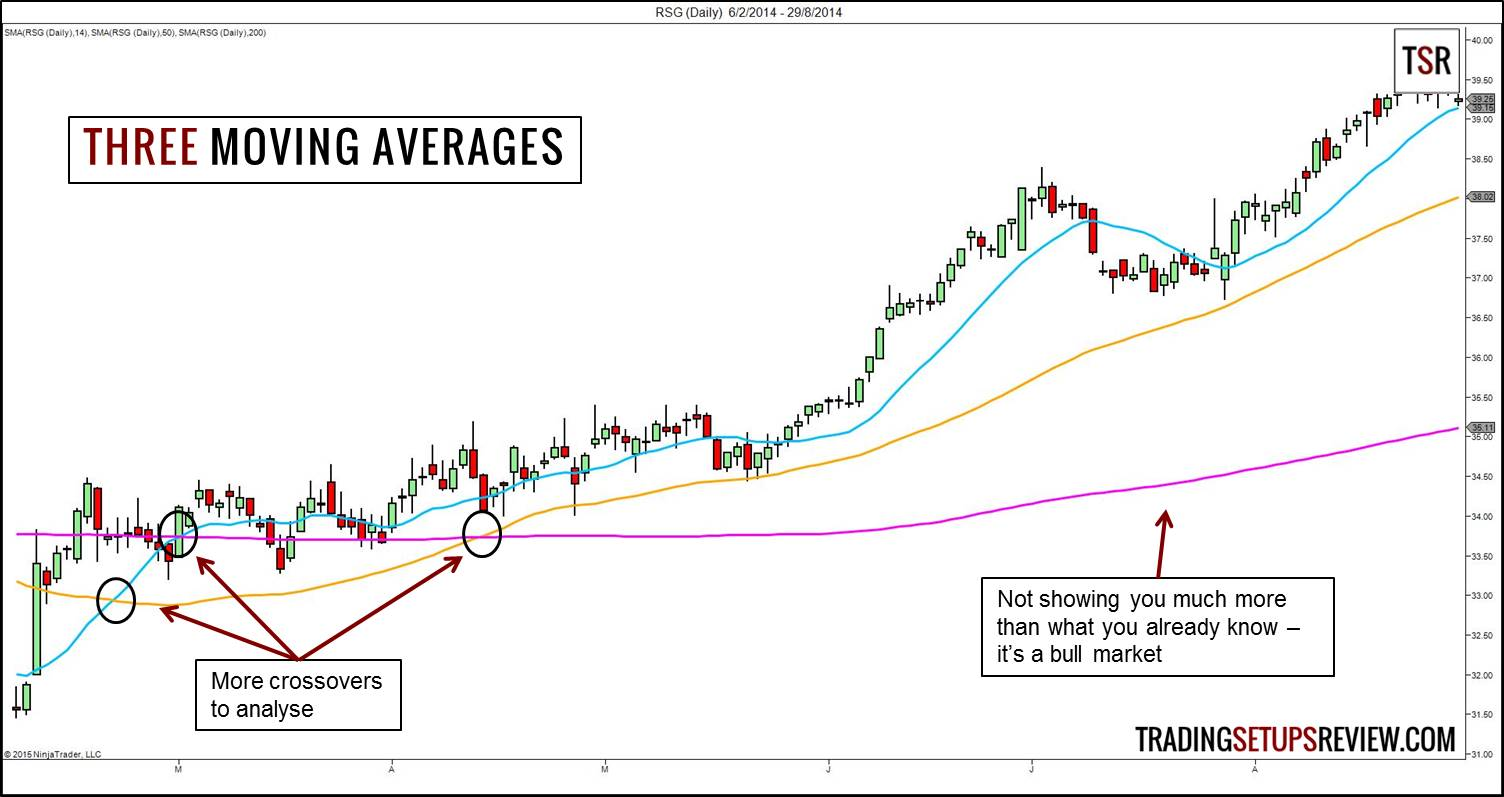
\includegraphics[width=1.0\textwidth]{img/multiple-technical-indicators.jpg}
\label{figure:multiple-technical-indicators}
\end{figure}

% Explain that we use retracements
% Explain the whole enchilada: we add the duplicated fibos, we group them in
% zones of 10 pips, we do it for each price, etc.

\section{Using Agents to Represent Traders in a Financial Market}
\label{section:using-agents-to-represent-traders-in-a-financial-market}

Using an agent-based model to represent a financial market is perhaps one of the
most natural ways to do so. The explanation for this is that any financial
market is, in fact, being constructed by a group of agents: the traders. In the
proposed method, agents follow the process depicted in Figure
\ref{figure:agent-architecture}.


\begin{figure}
\caption{Architecture of an agent} \centering
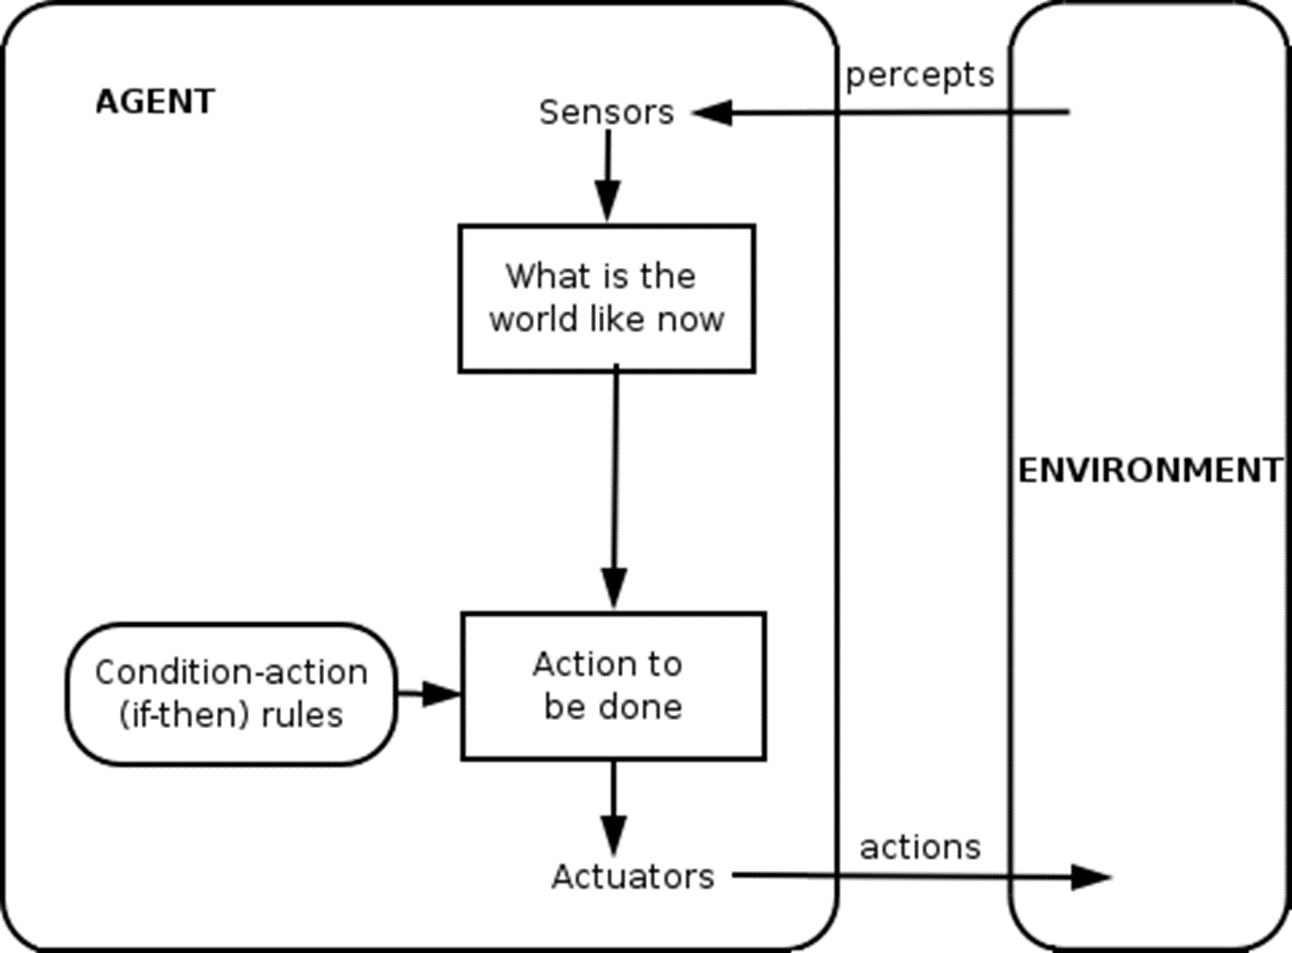
\includegraphics[width=1.0\textwidth]{img/agent-architecture.png}
\label{figure:agent-architecture}
\end{figure}

In this architecture, an agent is constantly sensing its environment, which, in
the case of this thesis, is the raw market prices coming from a broker. The
preprocessing mentioned in Section
\ref{section:preprocessing-a-financial-market-using-retracements} takes place as
part of each agent's sensing process; in other words, each agent has the
capability of preprocessing the market's raw data in their own fashion.

After preprocessing the raw data, each agent uses a set of rules in order to
decide if it should interact with its environment in a certain way. In this
case, this interaction takes the form of trades: the agent decides if it is
necessary to perform a sell or buy transaction for a particular number of units,
or if no action should be performed at all.

The collection of every agent's actions can provide a simulation of the next
market's price. This simulation is achieved by summing each of the agent's
response to the market. In other words, the simulated price for a time $t_0$ can
be obtained by the calculation represented by \ref{equation:sum-of-agents-units}:

\begin{equation}
  \label{equation:sum-of-agents-units}
  p_t0 = p_t-1 + \sum_{i=1}^{N} U_i
\end{equation}

where $p_t-1$ represents the previous price, i.e. the price for time $t_-1$, and
$U$ denotes the number of units an agent will trade at time $t_0$. The number of
units can either be positive or negative. This model can successfully represent
how a number of trades in different directions and magnitudes can move the price
of a market.

\section{Using Retracements to Represent the Beliefs of a Trader}
\label{section:using-retracements-to-represent-the-beliefs-of-a-trader}

As mentioned in Section
\ref{section:using-agents-to-represent-traders-in-a-financial-market}, each
trader in the agent-based model can have its own interpretation of the market,
represented by the preprocessing it performs on the market's raw price data. In
order to achieve these market interpretations, the proposed method follows the
ideas proposed by Shoham in \cite{Shoham1993}, where agents have a set of
beliefs that influence how they perceive their environment.

This work proposes that the beliefs of an agent can be represented by the
parameters of their environment preprocessing algorithm. As described in Section
\ref{section:preprocessing-a-financial-market-using-retracements}, retracements
are used to achieve this preprocessing in the proposed method, which means that
the agents in the agent-based model use as their beliefs a set of ratios that
are used to obtain the retracements in the market. These retracements are then
used to represent prices where the agent believes that a trade could be
initiated. As a consequent, even if two agents have the same trading strategy,
i.e the same rules, they can trade differently depending on how they perceive
the market according to their beliefs.

\section{Representing the Agents' Rules as Intuitionistic Fuzzy Systems}
\label{section:representing-the-agents-rules-as-intuitionistic-fuzzy-systems}

Another concept grabbed from Shoham's work described in \cite{Shoham1993} is
that agents have a set of commitment rules. These commitment rules -- or just
rules, as they will be referred as from now on -- determine what actions, if
any, will an agent perform on their environment.

Some works represent the agents' rules using simple if-then statements
\cite{Niazi2011} \cite{Pellizzari2007}. In contrast, the work in this thesis
uses intuitionistic fuzzy systems to represent the rules. The reason behind this
decision is that fuzzy systems are particularly useful for knowledge
visualization and interpretation. One can examine the membership functions in
the fuzzy rules to have an idea of how the fuzzy system will perform. This can
also be said about simple if/else statements, but fuzzy systems have the
advantage of being able to represent a virtually infinite number of if/else
statements in a simple way (through membership functions) and that they can
easily be optimized using a meta-heuristic algorithm.

In the proposed method, the outputs from the preprocessing algorithm serve as
inputs for the fuzzy system. For example, at certain time point in a market, one
can use the values of different moving averages as the inputs for the fuzzy
system of an agent. The outputs of the preprocessing algorithm are then
associated to a set of membership functions that act as the antecedents of an
inference system which, following the workflow of a common fuzzy system, fire
the membership functions that act as consequents which represents a number of
units that will be traded by the agent at a particular time in the market. It is
noteworthy that in this case Mamdani systems are being proposed to be used as
the agent rules (see Subsection \ref{subsection:fuzzy-systems}). This approach
also provides flexibility, as the system can easily be adapted to any number of
inputs coming from the preprocessing algorithm.

\subsection{Indeterminacy or Hesitancy}
\label{subsection:indeterminacy-or-hesitancy}

The fuzzy systems used to represent the agent rules are of a kind called
intuitionistic fuzzy systems (see Subsection
\ref{subsection:intuitionistic-fuzzy-systems}). This type of fuzzy system
provides an additional abstraction layer to the uncertainty that can be modelled
by traditional fuzzy systems, which is denoted as indeterminacy or hesitancy
\cite{Atanassov1986}. In the case of this work, hesitancy can be seen as doubt
in an agent's perceptions and actions. For example, an agent can be perceiving a
very strong resistance area in the market above the current price, but if the
membership function associated to that input is high, it can mean that the agent
is unsure of what it is perceiving. This perception can be described in words as
``the agent is very unsure of perceiving a high resistance above the current
price''. This previous statement also helps the understanding of the difference
between uncertainty and indeterminacy in an intuitionistic fuzzy system.

As an additional example, one can examine the intuitionistic fuzzy set depicted
in Figure \ref{figure:indeterminacy-in-an-agents-action}. If this fuzzy set
represents the action of an agent (the units to be traded), it can be seen that
the trader is doubtful about trading a moderate number of units. It can also be
seen that this doubt is located at the left of the membership function, which
will cause a trader to be doubtful about trading a below moderate number of
units or, in other words, it will be trading a higher than moderate number of
units. Indeterminacy in this case can model situations such as ``according to
what I'm perceiving, I should be conservative and trade the usual amount of
units. However, taking some additional risk could be worth it, so I will
increase my bet.''

\begin{figure}
\caption{Indeterminacy in an agent's action} \centering
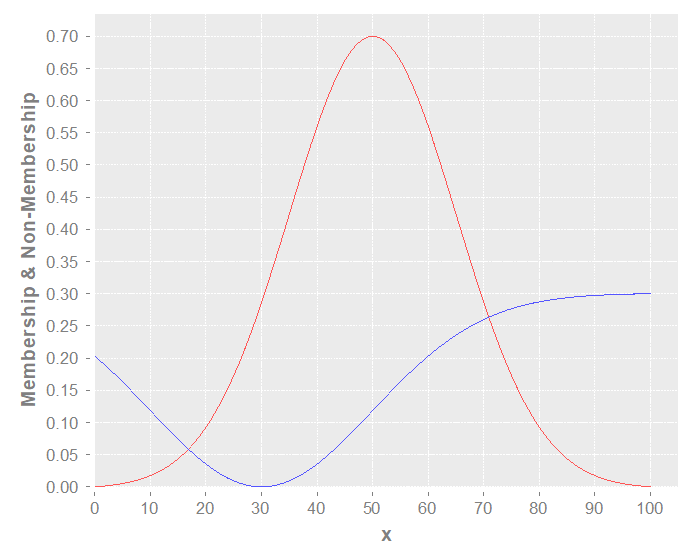
\includegraphics[width=1.0\textwidth]{img/example-of-ifs.png}
\label{figure:indeterminacy-in-an-agents-action}
\end{figure}

Indeterminacy is used in this work to further describe and understand how the
agents in the system are behaving in order to simulate the financial market. As
seen in the results presented in Chapter \ref{chapter:experiments}, a market
report is generated, which summarizes what the agents are perceiving and how
they are responding to their environment. This report also includes the
indeterminacy in these perceptions, which helps the reader understand the role
of doubt in the agents' decisions.

\section{Generation of an Agent-Based Model}
\label{section:generation-of-an-agent-based-model}

Previous Sections describe the architecture and behavior of an isolated
agent. This Section explains how multiple instances of the proposed agent
architecture create an agent-based model of a financial market.

As has been explained, an agent in the proposed method interacts with its
environment by issuing trade orders. These trade orders can be one of two
possible types: buy or sell. If an agent buys units of an asset, the price of
said asset rises. In contrast, if an agent sells units, the price declines. This
conception can be extended to multiple agents trading the same asset: if there
is a majority of units being bought in an asset, the price rises, and it
declines if the majority is selling the asset. The process aforementioned can be
used to create a simulation of a market, where the agents in a multi-agent
system need to be adjusted to create a zero-sum situation that fits the real
market prices. For example, if the price difference between the price at $t_n$
and the price at $t_n+1$ is -10 units, the sum of the units traded by all the
agents must be equal to those -10 units.

In the case of simulating a single price, the adjustment of the multi-agent
system becomes trivial, but the complexity of the model grows exponentially as
more prices are added to the simulation. If one price is added, the system needs
to be able to simulate it correctly and all the previous prices, i.e. the
readjustment not only needs to consider the new price, but all the prices as a
whole.

This work proposes that a meta-heuristic is used to find a combination of
parameters that adjusts the multi-agent system in order to perform a
sufficiently good simulation of a real market. This combination of parameters is
composed of the beliefs and the rules of all the agents in the system. One way
to achieve exploitation in the meta-heuristic is to recombine the beliefs and
the rules among each of the agents, however, the exploration capacity of the
algorithm would be limited, as this situation would be similar to performing
crossover on a single chromosome. This becomes clearer after remembering that
each of the agents do not correspond to a solution to the system, but rather
every agent in the system create a solution or a model. As a consequent,
multiple communities of agents need to be created, and the collections of
beliefs and rules of each of the agents in the communities of agents are used in
the recombination process of the meta-heuristic.

The performance of a community of agents can be determined by any function that
can be used in curve-fitting problems, such as the mean-squared error. The
multi-agent to be evaluated is executed to simulate a set of prices that
correspond to a real financial market, and this simulation is then compared to
the real prices. It is not critical for the system to achieve a low
curve-fitting error (for example, a low mean-squared error), as it is desirable
for the system to provide a generalized model of the market. In other words, one
should not seek an overtraining situation, as the system will not be able to
correctly extrapolate its simulation to similar situations.

\section{Using the Agent-Based Model to Generate Insights about a Financial
Market}
\label{section:using-the-agent-based-model-to-generate-insights-about-a-financial-market}

Once an agent-based model of a financial market has been created, this model can
be examined to obtain information about the market. This process is possible
thanks to the agent-based architecture of the model, as the beliefs of the
agents provide an abstraction of what the traders in the real market are
perceiving, and the rules of the agents tell an explanation of the behavior of
the traders. Furthermore, as has been explained in Section
\ref{section:representing-the-agents-rules-as-intuitionistic-fuzzy-systems},
using an intuitionistic fuzzy system to represent the rules of an agent is
helpful in breaking down the different factors that guided an agent to a
decision.

The proposed method can specifically help the user to understand the following
characteristics of the market:

\begin{itemize}
\item \label{item:agents-perception} The number of agents that are perceiving
  the market in some way.
\item \label{item:agents-decisions} The number of agents that are taking certain
  decision according to what they perceived.
\item \label{item:agents-profit} The generated profit per agent in each of the
  training or testing datasets.
\item \label{item:agents-doubt} How doubt or hesitancy is influencing an agent's
  perceptions and decisions
\end{itemize}

\ref{item:agents-perception} is obtained by examining the agents beliefs and/or
the outputs of the preprocessing algorithm associated to these
beliefs. Considering the retracements preprocessing algorithm explained in
Section \ref{section:preprocessing-a-financial-market-using-retracements}, one
can calculate how many agents perceived that a market was experiencing a strong
resistance above the current price, for example. Furthermore, this calculation
can be extended to determine the percentage of the times where these agents
perceived this resistance. In a similar fashion, \ref{item:agents-decisions}
helps the user to describe the trading decisions of the agents: one can
calculate how many agents decided to buy at certain time in the market, and it
can be extended to determine what percentage of the time those agents decided to
take that decision.

\ref{item:agents-profit} is useful to determine the efficacy of an agent, as in
the end one is interested in examining the behavior of the agents that generated
a greater profit than the others, in order to follow its recommendations; or
maybe one can be interested in examining those who performed badly, in order to
avoid taking similar decisions.

Finally, \ref{item:agents-doubt} allows the system to express how sure were the
agents about their perceptions or trade decisions. One can use this doubt
measurement to decide if an economic bubble is approaching, for example, as this
economic phenomenon is caused by factors that are exogenous to the nature of the
financial market \cite{Martin2011}.

\section{Using the Agent-Based Model to create a Trading Strategy}
\label{section:using-the-agent-based-model-to-create-a-trading-strategy}

Using the multi-agent system as a trading strategy is straightforward. After
the system has undergone through the optimization process, it should represent a
generalized model of a financial market. The system is adjusted for a training
dataset, but if a different dataset

\chapter{Implementacion}
\label{chapter:implementation}

El siguiente conjunto de secciones describen la implementacion del metodo
propuesto segun las explicaciones presentadas en el Capitulo
\ref{chapter:proposed-method}. La implementacion propuesta utiliza un software
de simulacion como el mostrado en \cite{} (\url{}), este software de simulacion esta
programado en Unity con codigo fuente en lenguaje C\# de Visual Studio.

\section{Codificando los diccionarios de piezas}
\label{section:piece_dictionary}

La primera parte que se desarrollo para poder integrar el listado de piezas al
sistema de generacion fue decir la manera en como se establecerian las
diferentes piezas como las mostradas en la figura \ref{figure:game-basic-blocks}
del Capitulo \ref{chapter:proposed-method}, para esto se tomaron enncuenta
varias posibilidades, la primera, como se explica en la seccion
\ref{subsection:objectorientedidea} se buscaba ordenar las diferentes piezas
como diccionarios que contuvieran una o mas referencias a las piezas que
integraban cada entrada del diccionario, para esto las primeras 11 posiciones
eran elementos individuales uno para cada pieza como el mostrado en la figura
\ref{code:dic_individual_piece}, en el codigo se aprecia la manera en como se
designaba una pieza del juego, para poder trabajar de manera dinamica para poder
agregar mas compuestos segun fuese necesario se utilizaban dos diccionarios
extra, estos contenian los datos de los tipos de materiales posibles y la
informacion de los tamaños de las piezas, de esta manera en caso de tener mas de
una pieza en algun punto del diccionario era posible modificar el valor de
offset de cada una de las piezas calculando la distancia del punto central de
cada pieza al centro de todo el conjunto.

\begin{listing}[t]
  \begin{minted}[frame=lines, framesep=2mm,baselinestretch=1.2,fontsize=\footnotesize,linenos]{python}
    BLOCKS = {
      0: [
          {'type': BLOCK_TYPE['Circle'],
          'material': BLOCK_MATERIAL['wood'],
          'offset': [0, 0, 0] # x, y, z - Calculated from the center of the figure
          }]
    }

    BLOCK_TYPE = {
    'Circle': {'height': 72, 'lenght': 72},
    'RectTiny': {'height': 22, 'lenght': 42},
    'RectSmall': {'height': 22, 'lenght': 42},
    'RectBig': {'height': 22, 'lenght': 42},
    'RectMedium': {'height': 22, 'lenght': 42},
    'RectFat': {'height': 42, 'lenght': 82},
    'SquareTiny': {'height': 22, 'lenght': 22},
    'SquareSmall': {'height': 42, 'lenght': 42},
    'Triangle': {'height': 72, 'lenght': 72},
    'TriangleHole': {'height': 82, 'lenght': 82},
    'SquareHole': {'height': 82, 'lenght': 82}
    }

    BLOCK_MATERIAL = {
        'wood': 0,
        'stone': 1,
        'ice': 2
    }
  \end{minted}
  \caption{Ejemplo de diccionario con un solo elemento}
  \label{code:dic_individual_piece}
\end{listing}

De esta manera como se explico anteriormente era mas sencillo crear compuestos,
sin embargo, la desventaja que conyevaba utilizar este metodo era que no podiar
realizar modificaciones a las restricciones de las piezas, es decir, en caso de
querer evitar que un conjunto de piezas con determinados materiales no fuesen
generados no se tenia la facilidad de impedir este tipo de combinaciones.

En luz de esta informacion se opto por utilizar el metodo en base a clases
mencionado en la seccion \ref{subsection:classorientedidea}, el codigo
\ref{code:dic_individual_piece} muestra la nueva estructura utilizada segun el
diagrama de clases presentado en la figura \ref{figure:pieces-class-diagram},
deacuerdo a el diagrama presentado una clase base con las operaciones y
propiedades necesarias funcionaria como una clase \textit{padre} para las clases
de piezas particulares, de esta manera los individuos se representaran como un
conjunto de referencias a las clases que deben de ser generadas para la
composicion de niveles, sin embargo, esta manera de representar a los individuos
no contempla las restricciones que pueden ser definidas para la combinacion de
piezas-materiales, debido a esto se opto por genar una lista global que
mantuviera un record de las restricciones aplicadas en el sistema, y al momento
de generar cada reinstanciacion de clase para los indiciduos esta informacion se
pasara a las clases segun fuese requerido, en el codigo se presenta una variable
con el nombre \textit{mat}, esta variable tomara una lista de 3 valores que
define si alguno o algunos de los materiales no puede ser utilizado al momento
de asignar las clases a los individuos, al momento de encontrar una pieza que de
la coincidencia no puede ser utilizada con ningun material se eliminaran los
datos de la pieza generada y se pedira al sistema genere otra de manera aleatoria.

\begin{listing}[ht]
  \begin{minted}[frame=lines,framesep=2mm,baselinestretch=1.2,fontsize=\footnotesize,linenos]{python}
    class Circle(Piece):
      def __init__(self, mat, x=0, y=0, r=0):
          self.Name = "Circle"
          self.Height = 75
          self.Width = 75
          Piece.__init__(self, x, y, r, mat)
          self.update_values()
  \end{minted}
  \caption{Ejemplo de estructura de las clases hija que heredan de la principal}
  \label{code:dic_individual_piece}
\end{listing}


\section{Creacion de compuestos}
\label{section:composite_creation}

Una vez definidas las clases particulares que controlaran la informacion de las
piezas en el algoritmo se procede a definir la manera en como se entregaran y
controlaran los diferentes compuestos de piezas, para terminos mas simples los
compuestos son grupos de una o mas piezas y se mostraran a manera de diccionario
de listas como se muestra en el codigo \ref{code:dic_composites}, de esta manera
cada entrada en el diccionario tiene por nombre o apuntador el valor posicion
segun se fueron agregando al diccionario mientras que el contenido es una lista
con tuplas donde se estipula la informacion pertinente de cada pieza en el
compuesto, un ejemplo claro es el elemento en la posicion \textit{9} el cual
cuenta con 3 piezas que muestran los valores de offset medida desde el centro
del compuesto visto graficamente en el juego, esta lista se utiliza para
mantener un control de los compuestos que se pueden ir agregando durante la
ejecucion del algoritmo, de tal manera que las clases auxiliares de
\textit{Composite} creadas haran referencia a una o mas piezas segun la lista se
haya proporcionado al crear el compuesto.

\begin{listing}[ht]
  \begin{minted}[frame=lines,framesep=2mm,baselinestretch=1.2,fontsize=\footnotesize,linenos]{python}
    Composites = {
      0: [("RectTiny", 0, 0, 0, "wood")],
      1: [("RectSmall", 0, 0, 0, "wood")],
      2: [("RectMedium", 0, 0, 0, "wood")],
      3: [("RectBig", 0, 0, 0, "wood")],
      4: [("RectFat", 0, 0, 0, "wood")],
      5: [("SquareSmall", 0, 0, 0, "wood")],
      6: [("SquareHole", 0, 0, 0, "wood")],
      7: [("Circle", 0, 0, 0, "wood")],
      8: [("TriangleHole", 0, 0, 0, "wood")],
      9: [("RectBig", 100, 5, -27, "wood"), ("RectBig", -100, 5, 27, "wood"), ...
            ...("RectSmall", 0, 0, 90, "wood")]
    } 
  \end{minted}
  \caption{Diccionario con los compuestos existentes}
  \label{code:dic_composites}
\end{listing}

\section{Definicion de clase auxiliar de individuo}
\label{section:definition_of_clases}

Mediante el uso de la clase de composite se tiene un mejor control de los genes
que conformaran cada individuo de la poblacion, una vez que se tiene este
aspecto controlado el siguiente paso es el de crear programar la clase que
llevara el control de los cromosomas de un individuo, siendo los cromosomas los
compuestos asignados a cada individuo particular, de tal manera que un individuo
dentro de la informacion de cromosomas hara referencia a otra lista de
compuestos, la manera en como un \textit{Individuo} relaciona los compuestos es
mediante el uso de la linea de codigo:

\begin{minted}{python}
  chromosome_objects = [Composite(Composites[composite]) for composite in self.chromosome]
\end{minted}

Mediante esta linea de codigo se indica que se debera de crar una lista en donde
cada elemento sera una instancia de un compuesto asignado al individuo, de esta
manera si se requiere modificar la posicion o materiales de un compuesto
particular en el individuo es posible hacerlo desde la clase de
\textit{individuo}, de igual manera esta clase tiene como funciones principales
como se muestran en el diagrama de clase de la figura
\ref{figure:individual-class-diagram} realizar los calculos de fitness y generar
las listas de piezas que seran utilizadas para generar los archivos de salida
necesarios para las simulaciones de los niveles generados.



\section{Generacion de individuos}
\label{section:ind_generation}

Una vez definida la manera de controlar las clases el paso siguiente es el de
comenzar con la generacion de ls individuos de la poblacion, para poder lograr
esto se creo una linea de codigo en la cual los puntos necesarios para la
generacion de los individuos se entregan totalmente, esta linea de codigo en
cuestion es como sigue: 

\begin{minted}{python}
  pop = [Individual(chromosome = get_random_chrom(ind_pieces), ..
    ..mask = create_new_mask(ind_pieces)) for i in range(population)]
\end{minted}

Mediante el uso de esta linea de codigo se le indica al sistema que se requiere
una lista que representara a los individuos de la poblacion, cada elemento de
esta lista sera una instancia independiente de la clase \textit{Individual},
para generar esta instancia de clase es requerido dos valores siendo estos
primero una lista de valores numericos que representan cuales piezas se
asignaran a los individuos, para generar esta lista se utiliza una funcion como
se muestra en el codigo \ref{code:get_random_chrom}, el segundo dato requerido
es una segunda lista que denota una mascara mediante la cual las piezas
asignadas seran acomodadas al momento de generar los archivos de simulacion,
finalmente la ultima seccion del codigo - \textit{for i in range(population)} -
denota que el proceso se debera de repetir una cierta cantidad de veces, es
decir que pada cada individuo se generara una instancia con valores diferentes a
los anteriores, la cantidad de vences que se debera de repetir depende de la
cantidad de individuos con los que se quiere estar trabajando en el algoritmo en
el caso de las pruebas realizadas se utilizo un totoal de 10 individuos lo que
significa que la lista \textit{pop} generada consta de 10 instancias diferentes
de la clase \textit{Individual}. 

Para la generacion de la lista de piezas o cromosomas asignados a un individuo
mostrada en la parte (1) del codigo en \ref{code:get_random_chrom}, aqui el
valor que se recive denota la cantidad de piezas o compuestos que se deberan de
asignar en la lista para el individuo, para asignar estos valores primero se
obtine un numero aleatorio que va desde \textit{0} hasta la cantidad de piezas o
compuestos presentes en la lista menos una unidad para evitar errores de
posicionamiento de lista, posteriormente se revisa si la pieza seleccionada
puede ser utilizada almenos en una combinacion dentro de la generacion, en caso
de que no puede ser utilizada se obtiene otra y de igual manera se revisa, en
caso de poder ser utilizada se agrega a la lista y avanza un contador para saber
cuando se llegue al limite de piezas posibles de usar, finalmente se entrega la
lista de piezas para la generacion de la instancia de clase. Para la generacion
de la mascara de acomodo de piezas se utiliza la seccion de codigo mostrado en
la parte (2), en esta parte lo que se realiza es que se revisa la cantidad de
compuestos que se pueden utilizar como en la parte anterior, este valor se
utiliza posteriormente para generar una lista aleatoria, la lista que se genera
tiene un total de 7 posiciones que denotan 7 divisiones que se realizan en el
area de un nivel para el acomodo de las piezas, mediante el uso del valor de
piezas en cada individuo se realiza una aleatorizacion de numeros desde
\textit{0} hasta la cantidad maxima de piezas, una vez se obtienen estos valores
aleatorios se revisa si la suma de estos da la cantidad de piezas en el
individuo, en caso de que no sea asi se repite el proceso, en caso de que si se
cumpla entonces la lista se regresa para la creacion de la instancia de clase.

\begin{listing}[ht]
  \begin{minted}[frame=lines, framesep=2mm, baselinestretch=1.2, fontsize=\footnotesize, linenos]{python}
 (1)  def get_random_chrom(sl):
        asl = 0
        chrom = []
        while asl < sl:
            prop = random.randint(0, len(Composites)-1)
            if clases[Composites[prop][0][0]].Valid == True:
                chrom.append(prop)
                asl += 1
        #random.randint(0,len(Composites)-1) for p in range(ind_pieces)
        return chrom

 (2)  def create_new_mask(pieces):
        div_list =[]
        while True:
            div_list = [random.randint(0, pieces-1) for col in range(7)]
            if sum(div_list) == pieces:
                break
          
        return div_list
  \end{minted}
  \caption{Codigo de asignacion de cromosomas(piezas)[1] y codigo para generar mascaras [2]}
  \label{code:get_random_chrom}
\end{listing}

Una vez que se ah logrado cear la lista de individuos se procede a inicializar
el algoritmo evolutivo, este algoritmo se ejecutara una determinada cantidad de
veces que se haya establecido en el codigo, el pseudo-codigo ah ejecutar con su
respectiva implementacion en codigo se enlista a continuacion en el codigo
\ref{code:algorithm_pseudocode}, este pseudocodigo engloba los aspectos
principales del sistema de generacion de niveles, el codigo se explica mas a
detalle en las secciones siguientes.

\begin{listing}[ht]
  \scalebox{.8}{\noindent%
\begin{Heardlisting}{%
   \begin{tabular}{r}% 
      Integrar miembros "elite" (1-4)\\ \\  \\  \\  \\
      Simular individuos (6)\\  \\
      Calcular fitness (8-9)\\  \\  \\
      Obtener padres de la generacion (10)\\  \\
      Realizar crossover (12)\\ \\
      Seleccionar elite (14-15)\\ \\
   \end{tabular}
}
if elite not null
   for member in elite
      population <- member
      trim population

execute process (game)

for individual in population
   individual.getfitness

parents <- selector_operator(population, required)

crossover_operation(population, parents)

population.order('fitness')
elite.add(population[1])
\end{Heardlisting}}
  \caption{Pseudo-codigo del algoritmo genetico}
  \label{code:algorithm_pseudocode}
\end{listing}

\subsection{Integracion de miembros elite}
\label{subsection:elite_member_integration}

Esta parte se encarga de iniciar los bucles de generacion, la funcion principal
de este broque de codigo es la revisar la lista auxiliar de miembros de elite
que existe en memoria, en caso de tener elementos en la lista estos se integran
a la lista de la poblacion integrandose al inicio de la misma, una vez agregados
todos los miembros la lista de la poblacion se corta hasta el numero maximo de
miembros permitidos en las generaciones, este valor se asigna como un valor de
entrada al inicio del archivo que contiene el codigo.

Una vez terminada esta accion se procede a denotar la cantidad de padres que
seran necesarios para generar los hijos de las generaciones futuras, esto se
hace mediante el calculo:
\begin{minted}{python}
  many = len(pop) * per_cross
\end{minted}
En donde \textit{pop} representa la lista de miembros de la poblacion,
\textit{per\_cross} representa un valor entre \textit{0\.0} y \textit{1\.0}, este
valor representa que tanto porcentaje de la poblacion se quiere realice cruces,
de esta manera la variable \textit{many} representa la cantidad de individuos
que se deberan de utilizar para cumplir el porcentaje de cruce, debido a que el
valor de \textit{per\_cross} puede generar un valor flotante se tiene una parte
de codigo en donde si el total de individuos que realizaran cruces es un numero
inpar entonces el valor que se debera de utilizar sera el numero par redondeado
hacia abajo, es decir, si de 10 individuos en la poblacion se quiere que un
total de individuos cercano al \textit{50\%} realizen un cruce entonces el valor
resultante para la variable \textit{many} seria de 5, en este caso lo que se
hace es restar 1 al resultado y despues se redondea hacia abajo, lo cual haria
que el numero de padres requeridos para los cruces sea de 4.

Una vez que se tiene el valor de los padres requeridos para los crces de la
generacion se procede a crear los archivos auxiliares de los individuos de la
poblacion, los archivos generados son en formato \textit{XML}, la informacion
que contienen estos archivos es la posicion, tipo y material de ls piezas que
seran utilizadas en el nivel, ademas de esto tambien contiene la informacion de
la cantidad y tipo de aves asi como de los enemigos que seran colocados, estos
archivos son almacenados en un folder en donde el software de simulacion se
encarga de obtenerlos y entregar los resultados despues de la simulacion.

Una vez que los archivos de simulacion han sido generados el algoritmo manda un
comando que manda la ejecucion del software de simulacion, el software en
particular cuenta con una ventan grafica en la que se puede apreciar los niveles
que se generaron o envolucionaron an caso de estar simulando archivos de una
generacion despues de la primera, de igual manera el software genera un archivo
en formato \textit{XML} similar al que se genera antes de la simulacion, la
diferencia entre ambos archivos es que el que es entregado despues de la
simulacion entrega los datos de posicion del ultimo estado registrado del nivel,
ademas de que se puede solicitar que entregue el valor de la aceleracion de la
misma, el valor de aceleracion es tomado en cuenta desde el punto en el que la
pieza comienza su descenso, en caso de que una pieza sea destruida durante el
proceso de simulacion ninguno de los datos de esa pieza son grabados en los
archivos, la manera de llevar control de las piezas que entran y las que salen
es mediante el uso de un numero de lista asignado al momento de generar los
archivos de simulacion de la seccion anterior.

Posterior a la simulacion los archivos entregados son revisados y en base la
informacion de las piezas se calcula el \textit{Fitness} de las mismas,
posterioremente a esto se procede a ordenar la lista, y realizar las operaciones
de seleccion, cruce, mutacion los cuales se explican en la seccion siguiente.

\subsection{Operador de seleccion}
\label{subsection:sel_operator}

El proceso de seleccion se definio de dos maneras diferentes, la primer es
mediante el uso de una ruleta para las seleccion, en esta ruleta los valores que
se toman en cuenta es el fitness de cada individuo, mientras mas alto sea el
fitness mayor sera la probabilidad de ser seleccionado para el cruce en la
siguiente seccion.

El segundo metodo utilizado es la seleccion mediante torneo, en este tipo de
seleccion lo que se realiza es que los individuos se seleccionan en pares de
manera aleatoria, entre cada par se realiza un calculo de cual tiene el mejor
fitness y ese individuo es seleccionado como padre para la generacion.

\subsection{Operador de cruce}
\label{subsection:crossover_operator}

Para los operadores de cruce se tienen codificados dos tipos, cruce de un punto
y cruce de dos puntos, este operados de cruce se realiza no solo en elos
individuos de la poblacion sino tambien en las mascaras que tienen los mismos
individuos, esto es para aumentar un grado mas el nivel de diversidad que se
puede tener en los individuos generados, la idea en este caso es lograr que
existan casos en donde la mascara sea muy chica y varias piezas de los
individuos no sean mostradas y el caso contrario permitira que un individuos
pueda o no quedar con el mismo caso y puede que se de el caso en donde alguno de
ambos elementos logre obtener un mejor nivel de fitness en la generacion.

Un ejemplo de estos dos tipos de cruce se puede apreciar en la figura
\ref{figure:crossover} en donde dos individuos realizan un cruce con sus
mascaras y las mascaras generadas para los hijos resultan con diferente cantidad
de piezas.

La manera en como se aplican estsos tipos de operador es:
\begin{enumerate}
  \item Definir un punto de corte igual para los dos individuos en cualquier
  posicion de la lista de genotipos.
  \item Separar las dos partes cortadas de ambos individuos de tal manera que se
  tenga la parte de inicio (del inicio hasta el corte) y la parte final (desde
  el corte hasta el final) de cada individuo.
  \item Para crear al primer hijo tomar la parte inicial del primer individuo y
  unirla con la parte final del segundo individuo
  \item Para el segundo hijo tomar la parte inicial del segundo individuo y
  unirla con la parte final del primer individuo.
\end{enumerate}
De esta manera los hijos se pueden comprender de la siguiente manera:
\begin{minted}{python}
  padre1 = padre[1, punto_corte]
  padre2 = padre[punto_corte, fin]

  madre1 = madre[1, punto_corte]
  madre2 = madre[punto_corte, fin]

  hijo1 = padre1 + madre2
  hijo2 = madre1 + padre2
\end{minted}
Para el caso del cruce de dos puntos la manera en como se realiza es que en vez
de dividir el genotipo de un individuo en dos partes se divide en tres y al
momento de realizar la combinacion se toma la primer parte del primer individuo,
despues la parte de enmedio del segundo individuo y finalmente la parte final
del primero, de tal fomra que solo la parte central de ambos individuos se
cambia.

\begin{figure}
  \centering
  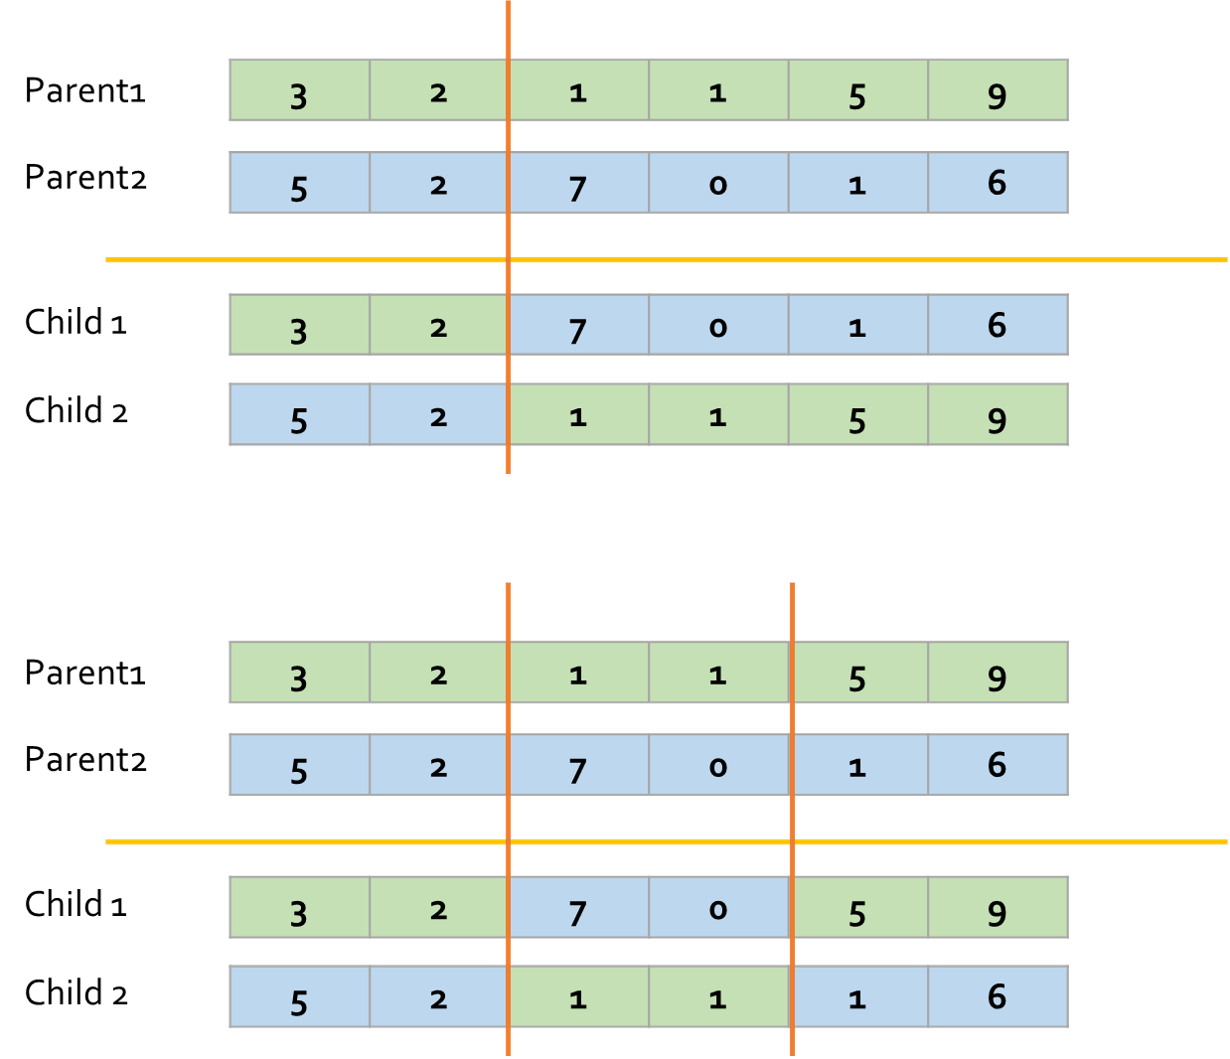
\includegraphics[width=0.8\textwidth]{img/crossover.png}
  \caption{Cruce de un punto (arriba) y cruce a dos puntos (abajo) aplicada a la mascara de individuos}
  \label{figure:crossover}
\end{figure}

\subsection{Operador de mutacion}
\label{subsection:mutation_operator}

La mutacion de los individuos de la poblacion ocurre solo al momento de hacer el
cruce de los mismos, es decir solo a los elementos nuevos se les aplica el
operador de mutacion, este operador puede modificar los siguientes elementos de
un individuo:
\begin{enumerate}
  \item La cantidad de piezas que conforman al individuo.
  \item El material del cual estan formados los elementos.
  \item El tipo de elemento que conforma a un individuo, es decir, modificar el
  valor del compuesto que forma parte del individuo.
  \item La posicion individual (\textit{x} o \textit{y}) de los compuestos.
\end{enumerate}

La manera en como se aplica el operador de mutacion se describe como sigue,
primero al momento de generar al nuevo individuo se realiza un calculo de
porcentaje en donde se decide si tendra o no mutacion dependiendo del procentaje
de mutacion que se haya asignado al inicio del algoritmo, posteriormente en caso
de que el valor de porcentaje quede dentro del rango se toma para las
operaciones, esta mismas se explican de la manera siguiente.

Para mutar la cantida de compuestos en un individuo primero se realiza una
seleccion aleatoria entre las opciones de agregar o quitar compuestos,
posteriormente en caso de requerir agregar mas se realiza una seleccion
aleatoria de entre la cantidad de compuestos creados, estos mismos se integran
al final de la lista de compuestos del individuo. Para eliminar elementos de la
lista se realiza una corrida por todos los elementos y en cada uno se realiza
una probabilida de \textit{50\%} de sea borrado de la lista, un ejemplo de este
proceso se muestra en la figura \ref{figure:mutate_add_remove} en donde se
presenta una tabla que denota las posiciones de los compuestos en base a la
mascara, en este ejemplo se realizo una corrida para remover elementos (color
rojo) y una segunda para agregar nuevos compuestos (color verde).

\begin{figure}
  \centering
  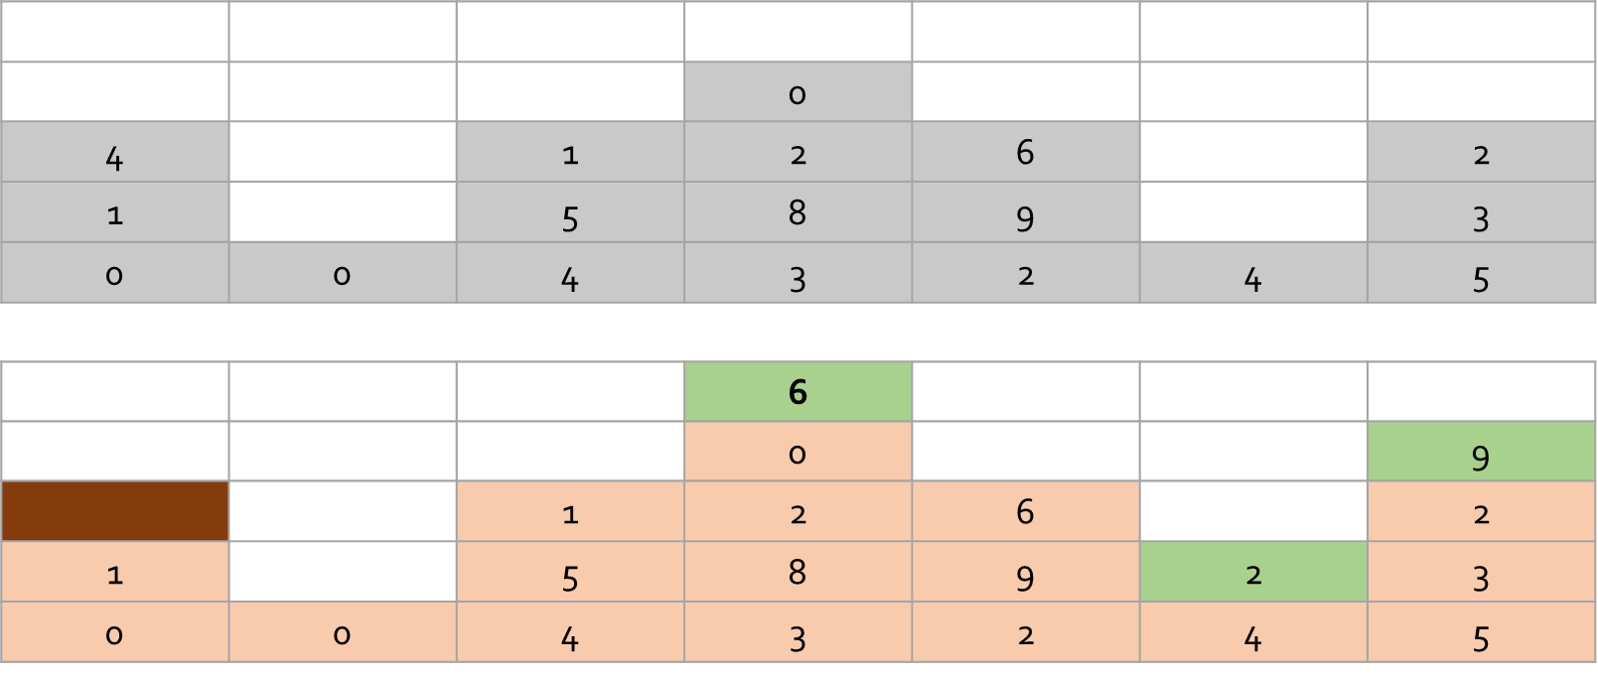
\includegraphics[width=0.8\textwidth]{img/mutation_add_remove.png}
  \caption{Ejemplo del operador de mutacion enfocado a remover y agregar compuestos}
  \label{figure:mutate_add_remove}
\end{figure}

La segunda mutacion se encarga de modificar el material del que estan
conformados los compuestos del individuo, la manera en como trabaja este proceso
es primero se selecciona aleatoriamente cuales compuestos seran modificados sin
repetir valores, posterioremente se modifica de manera aleatoria el valor que
define el tipo de material del que se conforma, para esto se toma en cuenta que
\textit{0} representa material de madera, \textit{1} representa material de
hielo y finalmente \textit{2} representa el material de piedra, debido a que el
juego solo acepta esta lista de compuestos no es posible asignar valores
diferentes a estos.

En la figura \ref{figure:mutate_material} se muestra un ejemplo de la manera en
como opera la mutacion del tipo de compuesto, en este ejemplo se muestra el
genotipo y fenotipo de un individuo, el genotipo muestra los colores naranja,
azul y gris para denotar los materiales de madera, hielo y piedra
respectivamente, en este caso la mutacion cambia el material de 5 elementos del
genotipo de madera a hielo, esto se refleja del lado derecho en donde se muestra
la vista actualizada del individuo despues de la mutacion.

Debido a que los compuestos generados pueden contener diferentes cantidades de
elementos en estos casos se cambia el material equitativamente a todos elementos
del compuesto, de esta manera se evita tener que realizar un recorrido por todo
el compuesto y mutar el material de cada uno.

\begin{figure}
  \centering
  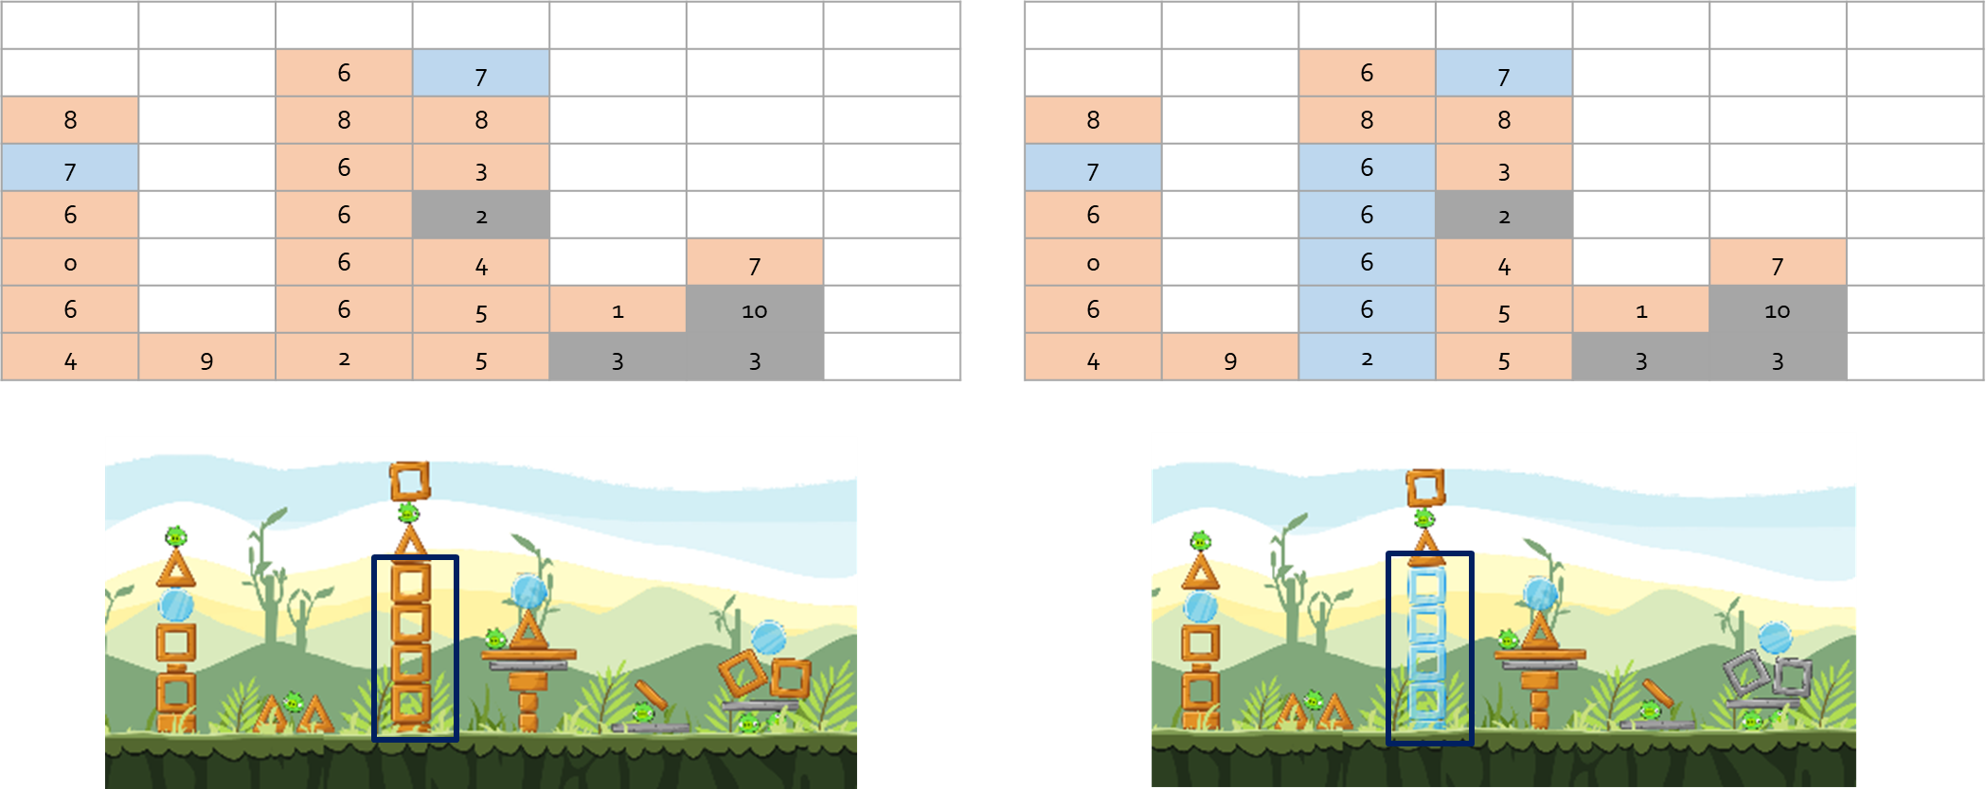
\includegraphics[width=0.9\textwidth]{img/mutation_material.png}
  \caption{Ejemplo del operador de mutacion enfocado a cambiar el material de los compuestos, pre-mutacion (izquierda) y post-mutacion (derecha)}
  \label{figure:mutate_material}
\end{figure}

La tercera mutacion se encarga de cambiar el compuesto que representa una
posicion del genotipo del individuo, este trabaja de una manera similar al
anterior en el sentido de que primero se selecciona a los individuos a mutar,
posteriormente a la seleccion se realiza una segunda seleccion aleatoria entre
las posiciones del genotipo del individuo, aquellos compuestos seleccionados son
cambiados por otro de la lista existente, para esto se realiza una seleccion de
un valor aleatorio que va desde \textit{0} hasta la cantidad de compuestos
existentes, por ejemplo suponiendo que se tiene solo la cantidad base de piezas
en el algoritmo entonces la seleccion sera un valor aleatorio desde \textit{0}
hasta \textit{10}.

La figura \ref{figure:mutate_composite} nos muestra un ejemplo de como es que
actua la mutacion de tipo de compuesto, en el ejemplo mostrado se tiene el
genotipo de un individuo combinado con su respectiva mascara asi como su
fenotipo respectivo (lado izquierda) al ser representado en la pantalla del
juego, en el lado derecho de la misma imagen se aprecia la modificacion de
compuestos realizada al genotipo base (marcado en amarillo), la modificacion de
compuestos en los individuos puede traer la conscuencia de que los niveles
generados sean inestables como en este ejemplo, esto a su vez puede permitir
identificar mascaras de los individuos que logran mantener la estabilidad de las
estructuras permitiendo asi mejorar el algoritmo.

\begin{figure}
  \centering
  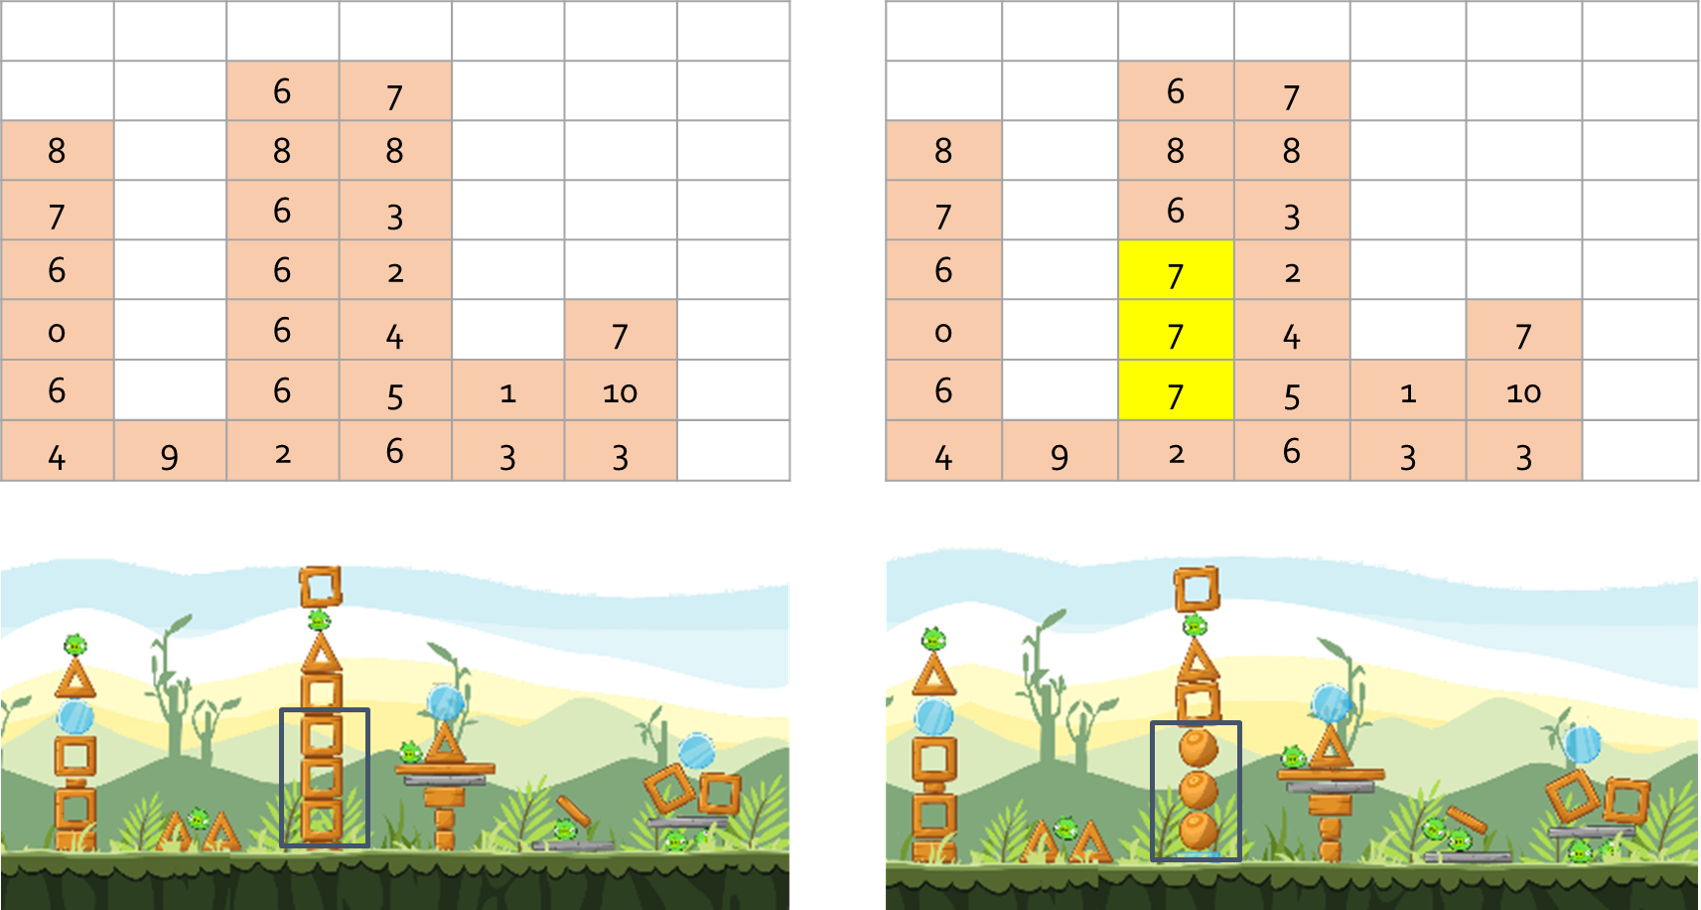
\includegraphics[width=0.9\textwidth]{img/mutation_composite.png}
  \caption{Ejemplo del operador de mutacion enfocado a cambiar los compuestos asignados, pre-mutacion (izquierda) y post-mutacion (derecha)}
  \label{figure:mutate_composite}
\end{figure}

El ultimo tipo de mutacion realizada en los individuos es la modificacion de las
posiciones \textit{x} y \textit{y} de algunos compuestos dentro del individuo,
la modificacion de las posiciones se realiza mediante una seleccion de valores
aleatorios de una distribucion gaussiana dentro de un cierto rango de distancia
para no permitir que los elementos se alejen demasiado de punto central
original.

\subsection{Representacion de individuos}
\label{section:individual_representation}

Una vez que se han agregado nuevos individuos a la poblacion, y que estos
individuos pasaron por su fase de mutacion si es que requerian se procede a
realizar la combinacion de los elementos que conforman al individuo con el fin
de generar los archivos requeridos para la simulacion de estos mismos, cabe
resaltar que esta combinacion se realiza tambien en los individuos iniciales
antes de la simulacion inicial, debido a que el juego requiere una
representacion mediante el uso de archivos en formatos \textit{XML}, se requiere
primero obtener la informacion de todos los elementos que conforman a un
individuo y posteriormente armar los archivos mediante el uso de estos datos.

\begin{figure}
  \centering
  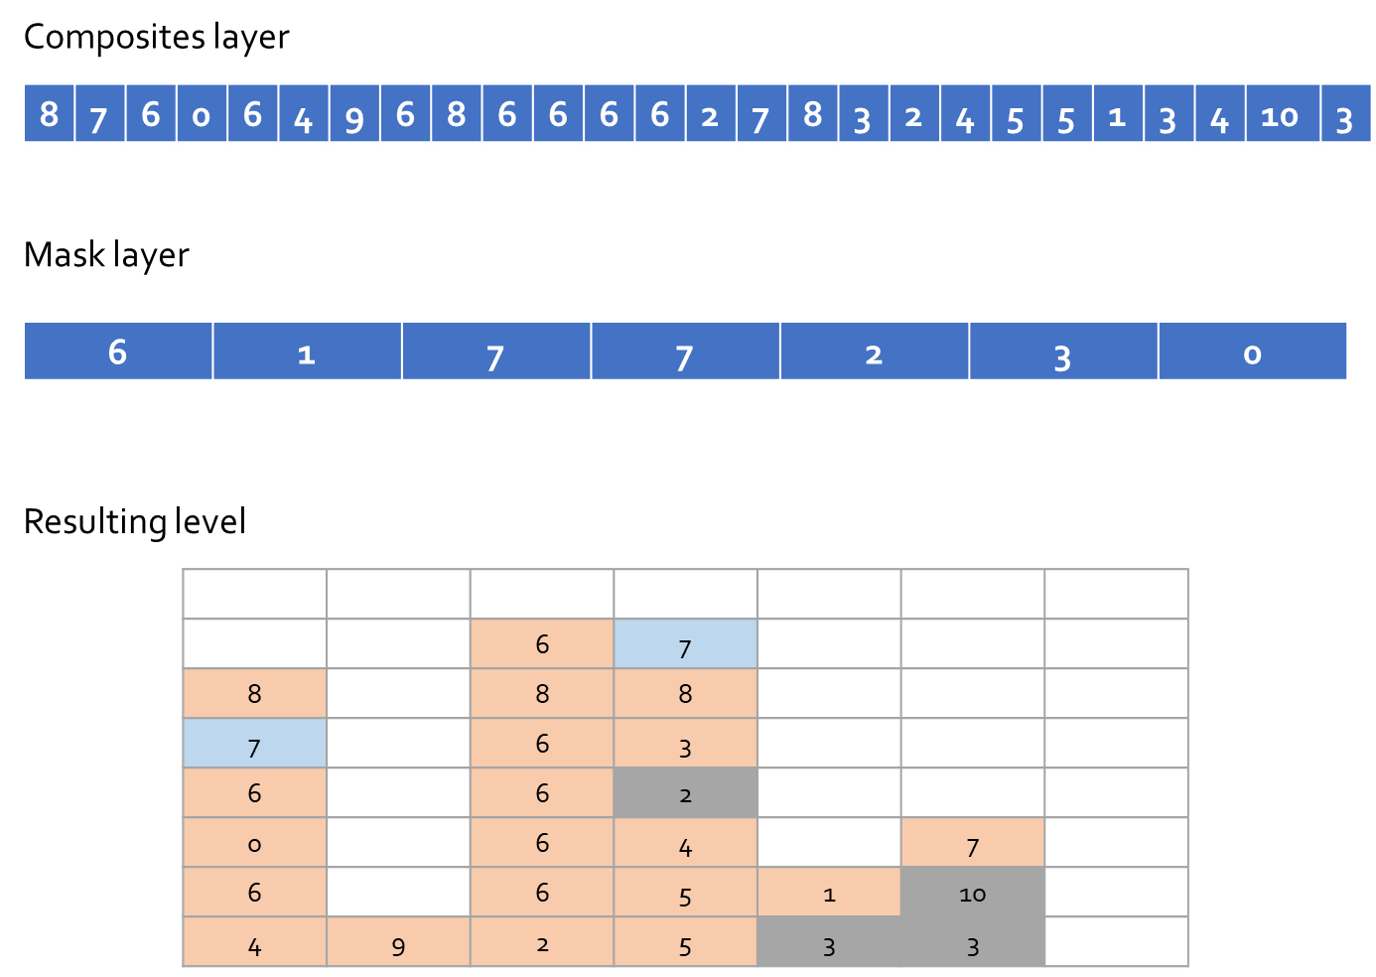
\includegraphics[width=0.9\textwidth]{img/layer12_combine.png}
  \caption{Ejemplo de la combinacion de capas de un individuo}
  \label{figure:individual_representation}
\end{figure}

En la figura \ref{figure:individual_representation} muestra la estructura de los
componentes de un individuo, un individuo es representado por \textit{2} capas
diferentes en forma de lista, la primera es la capa de compuestos, esta capa se
muestra la lista de compuestos que representan a un individuo, esta listas puede
variar en tamaño dependiendo de si durante las operaciones de mutacion se le
agregaron o quitaron elementos al individuo, de igual manera como se axplico en
el la seccion \ref{section:composite_creation} cada valor de la lista representa
no una pieza del juego sino uno de los compuestos que se crean antes de iniciar
el algoritmo o aquellos que se agregan durante el mismo en caso de haber.

La segunda parte que compone la representacion del individuo es la mascara, como
se explica en la seccion \ref{subsection:ruleofthirds} la idea detras del uso de
esta mascara es la de generar estructuras utilizando la lista de compuestos del
individuo, en esta misma seccion se presento una propuesta de crear mascaras en
donde se denotara la forma que se queria que tuviera un individuo particular,
aplicando estas estructuras en los individuos generaba los resultados esperados,
siendo el caso niveles en donde la distribucion de los compuestos crearan formas
diferentes como castillos, torres, casas o diferentes figuras, sin embargo
utilizar esta tipo de estructuras no permitia que el algoritmo lograra
evolucionar sino que simplemente encontraria la mejor combinacion de
piezas-mascara en determinado momento, por esto se opto por utilizar la
generacion de mascaras que se muestra en la figura
\ref{figure:individual_representation} y que fue explicado en la seccion
\ref{section:ind_generation} la cual unicamente muestra una determinada cantidad
de piezas a asignar en posiciones diferentes del nivel, esto permite tener mejor
diversidad en los individuos creados.

Al momento de combinar ambos componentes del individuo se obtiene un resultado
similar al mostrado en la parte inferior de la imagen en donde los compuestos se
organizan en manera de cola, es decir el primer elemento en la lista sera el
primero en ser colocado, una vez que se definen cuales elementos seran colocados
en cada columna el sistema calcula la altura total de cada compuesto y
comenzando desde la parte inferior coloca un compuesto en el nivel, despues
calcula la distancia desde la parte superior del mismo hasta la parte central
del siguiente para colocarlo de tal forma que al comenzar la simulacion no
aparescan en caida libre sino que aparescan una pieza sobre otra, de esta manera
se previenen problemas de balance al permitir que que las piezas caigan y
reboten en direcciones que provocaran que las estructuras terminen por caer
totalmente, en la misma imagen se aprecian cuadros de diferentes colores, estos
mismos representan el material del cual esta construido cada compuesto como se
explico en la seccion de mutacion anterior.

Finalmente una vez que se tiene la informacion anterior definida se procede a
realizar una busqueda de los lugares en donde apareceran los enemigos del juego,
la manera en como se define donde pueden aparecer estos es mediante una funcion
que revisa los compuestos que existen en el nivel, caundo un compuesto cumple
con ciertas caracteristicas se permite que uno de los enemigos pueda ser
colocado en la parte central o superiror del mismo, al iniciar este metodo se
busca aquellos que cumplen esta caracteristica y se ordenan en una lista
auxiliar, despues de manera pseudo-aleatoria se decide la cantidad de enemigos
que tendra el nivel, deacuerdo a este valor se seleccionan \textit{x} cantidad
de posiciones para colocar a los enemigos donde \textit{x} es el valor de
enemigos requeridos, una vez se definio en donde estaran colocados estos
enemigos se regresa una lista con las coordenadas \textit{x} y \textit{y} de las
mismas.

Mediante la combinacion de los enemigos con el genotico construido de un
individuo se obtiene el nivel a mostrar en el juego, una representacion de esto
se muestra en la figura \ref{figure:ind_representation_plus_pigs} en donde al
genotipo armado deacuerdo a los puntos anteriormente mencionados se le agrega el
listado de posiciones de los enemigos, en este caso los enemigos son
representados por un color verde en las posiciones en donde estaran, finalmente
esto permite tener la estructura de los niveles completa, esta informacion se
utiliza al momento de generar los archivos de \textit{XML} los cuales en el
software de simulacion generaran una vista de los mismos como se muestra en la
esquina inferior derecha de la misama imagen. 

\begin{figure}
  \centering
  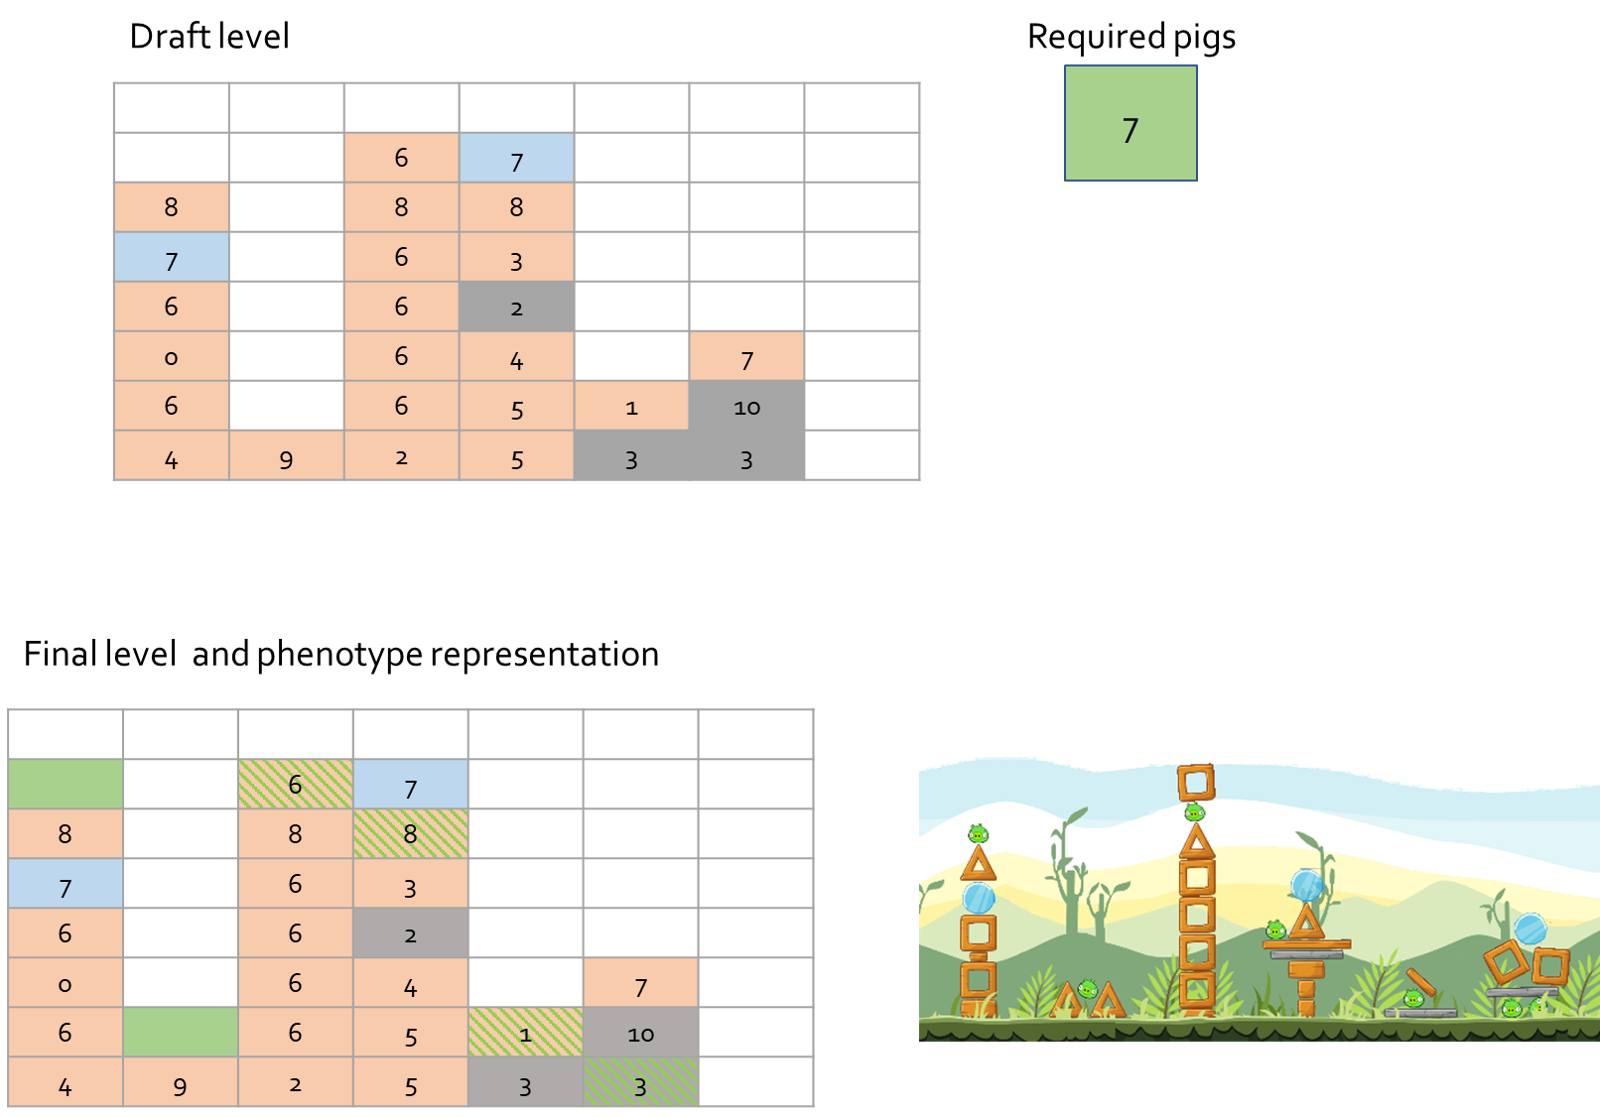
\includegraphics[width=0.9\textwidth]{img/layer123_combine.png}
  \caption{Ejemplo de la combinacion de un genotipo armado de la figura \ref{figure:individual_representation} con la colocacion de enemigos}
  \label{figure:ind_representation_plus_pigs}
\end{figure}

\subsection{Calculo de fitness}
\label{subsection:fitness_calculation}

Cuando los individuos pasan por el proceso de simulacion se genera un archivo en
formato \textit{XML} que contiene los resultados de los compuestos que fueron
puestos en los archivos antes de la simulacion con la diferencia de que estos
archivos contienen la informacion del ultimo estado de los mismos compuestos al
terminar dicha simulacion es decir se regra un listado de piezas y enemigos con
la informacion de sus posiciones \textit{x} y \textit{y} asi como del angulo con
en el cual quedaron al concluir la simulacion, ademas de esto se entrega la
informacion de la velocidad promedio de movimiento que tuvieron.

Esta informacion perimte conocer las inperfecciones que tuvieron los niveles al
concluir las simulaciones, para una mejor evaluacion de la aptitud de los
individuos se realiza una evaluacion que toma en cuenta los siguientes puntos:
\begin{itemize}
  \item La cantidad de piezas que no son destruidas durante la simulacion.
  \item La diversidad de las piezas utilizadas en el individuo.
  \item El resultado de la funcion de entropia con las piezas utilizadas.
  \item La distancia \textit{Hamming} del mismo conjunto de piezas.
\end{itemize}

Primero para realizar la evaluacion de la primera parte del calculo de aptitud
se toma el listado de piezas que se asigno al individuo antes de la simulacion,
ademas de esto se toma el listado de las piezas que resultaron despues de la
misma, posteriormente se realiza un calculo de procentaje de los valores de
ambas listas en donde la lista inicial representa el \textit{100\%} de la
aptitud del individuo, este calculo regresa un valor porcentual que se utiliza
como la base para las evaluaciones subsequentes, mientras mas piezas se
destruyan durante la simulacion el resultado de aptitud para el individuo sera
menor.

Despues de esto se realiza un calculo de los diferentes compuestos que integran
a un individuo, para la evaluacion de esta parte se toma en cuenta la diversidad
que logra tener el indiviudo, en donde el utilizar diferentes compuestos de la
lista total permite tener una mejor calificacion, esto es debido que mientras
mas compuestos sean utilizados los niveles que se pueden generar seran diversos
entre si.

Posterior a esto se realiza un calculo de la entropia de un individuo, el
calculo de entropia es utilizado en la teoria de informacion para calcular el
nivele de desorden o incertidumbre en los individuos, la formula que se utiliza
para esto se muestra en 

%\[ x^n + y^n = z^n \]

%\[ s = -\sum_i P_i \log P_i]
\chapter{Experiments and Results}
\label{chapter:experiments-and-results}

This Chapter describes a series of experiments that were performed in order to
demonstrate the capabilities of the proposed method regarding two areas:
forecasting and interpretability. The forecasting capabilities of the method are
demonstrated by exhibiting how the multi-agent model simulates the prices in
training and testing datasets, and how the system's curve-fitting error
decreased throughout the genetic algorithm's generations. The simulated profits
are also included, for both the training and testing datasets. These plots along
with some discussions of the results are provided in Section
\ref{section:forecasting-the-prices-of-a-financial-market}. Regarding the
interpretation capabilities of the method, a description of how the agents
perceive the market is shown. This description also describes what actions the
agents take according to their perceptions. These interpretations can be found
in Section \ref{section:extracting-insights-about-a-financial-market}, along
with their respective discussions.

All of the experiments were optimized for a total of 100 generations. The reason
behind this is that the number of experiments was relatively big for this
thesis document because of the combinations among the number of markets, number
of agents, number of rules and number of individuals. Additionally, some
undocumented experiments were showing a stagnation after the 100th generation
regarding error minimization.

The experiments cover the following variants in the parameters: 4 agents, 4
rules and 4 individuals; 10 agents, 10 rules and 10 individuals; 20 agents, 20
rules and 20 individuals; and these variants are used to created models for the
following foreign exchange markets: AUD/USD, EUR/GBP, EUR/USD, GBP/USD and
USD/CAD.

A total of 135 experiments were performed, but due to space constraints in this
thesis document, only some of the experiments are shown. Specifically, the
forecasting and interpretation Sections show results for the cases of 4 agents,
4 rules and 4 individuals; 10 agents, 10 rules and 10 individuals; and 20
agents, 20 rules and 20 individuals. Each of the aforementioned cases are
extracted for each of the five foreign exchange markets: AUD/USD, EUR/GBP,
EUR/USD, GBP/USD and USD/CAD. The reader can find the plots and interpretations
for all the experiments performed in the Git repository of this thesis here:
https://github.com/amherag/PhD-Thesis/.

\section{Forecasting the Prices of a Financial Market}
\label{section:forecasting-the-prices-of-a-financial-market}

This Section shows some experiments that have the goal of forecasting different
foreign exchange markets. Different agent-based models were generated using the
parameters indicated in each of the Subsection titles. The datasets used for the
training stage of the model comprehends the prices and timestamps associated to
each of these prices, from Monday, January 28, 2019 5:00:00 PM GMT-08:00, minus
20 hours that are required to generate the initial retracements (see Section
\ref{section:preprocessing-a-financial-market-using-retracements:implementation})
to Sunday, February 3, 2019 8:00:00 PM GMT-08:00. Regarding the datasets used
for the testing stage of the model, the data comprehends the prices and
timestamps associated to each of these prices, from Sunday, February 3, 2019
9:00:00 PM GMT-08:00, minus 20 hours that are required to generate the initial
retracements, to Friday, February 8, 2019 12:00:00 AM GMT-08:00. All the
datasets have a size of 100 data points, and they correspond to the prices of
the foreign exchange markets AUD/USD, EUR/GBP, EUR/USD, GBP/USD and USD/CAD
according to the corresponding experiments Section.

Each of the following Subsections shows five plots: two plots of the
curve-fitting of the optimized model for the training and testing datasets, two
plots of the profits generated by the simulated trades of the optimized models
for the training and testing datasets, and a plot of the error minimization in
the training or optimization stage. The titles of the plots for both the
training and testing stages also include the mean-squared error in parentheses
(denoted by $\epsilon$) for the simulated versus real prices. The profit plots
show the accumulated profits through time in asset units. The minimization plot
shows the mean-squared error obtained by the best individual in each of the
generations.

\newpage

\subsection{AUD/USD 4 Agents, 4 Rules, 4 Individuals}
\label{results:forecast-aud-usd-4agents-4rules-4individuals}

Figure \ref{figure:aud-usd-4agents-4rules-4individuals} shows the plots for the
agent-based model with the worse modelling capabilities for the foreign exchange
market AUD/USD. As can be expected, the model did not achieve good training or
testing profits, although the mean-squared error is considerably low. This can
be a sign of poor generalization capabilities of the model due to the low number
of agents and rules. Additionally, the low number of individuals can provide
cause bad exploration in the genetic algorithm.

\begin{figure}[htp]
  \centering

  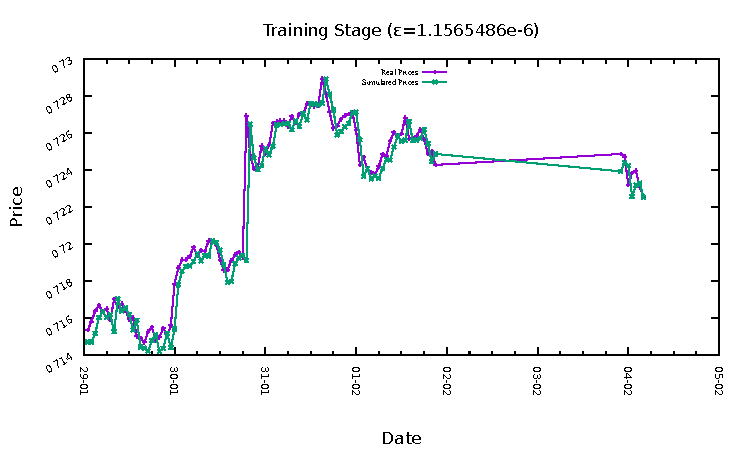
\includegraphics[width=.45\textwidth]{img/plots/aud_usd_h1-4agents-4rules-4ind-100gen_training_fit.pdf}\quad
  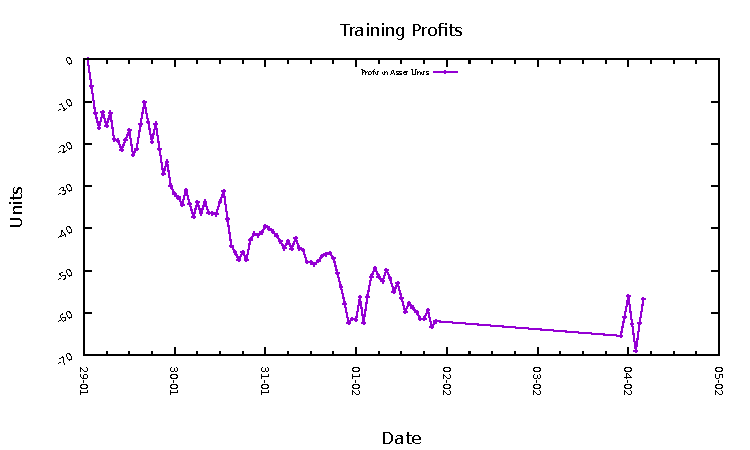
\includegraphics[width=.45\textwidth]{img/plots/aud_usd_h1-4agents-4rules-4ind-100gen_training_profits.pdf}

  \medskip

  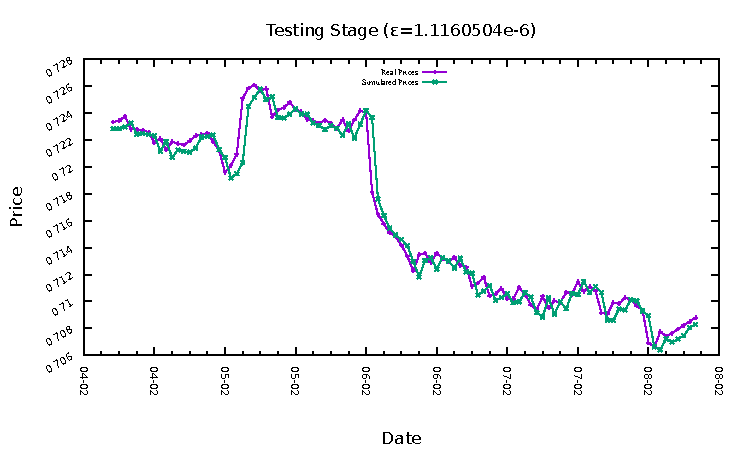
\includegraphics[width=.45\textwidth]{img/plots/aud_usd_h1-4agents-4rules-4ind-100gen_testing_fit.pdf}\quad
  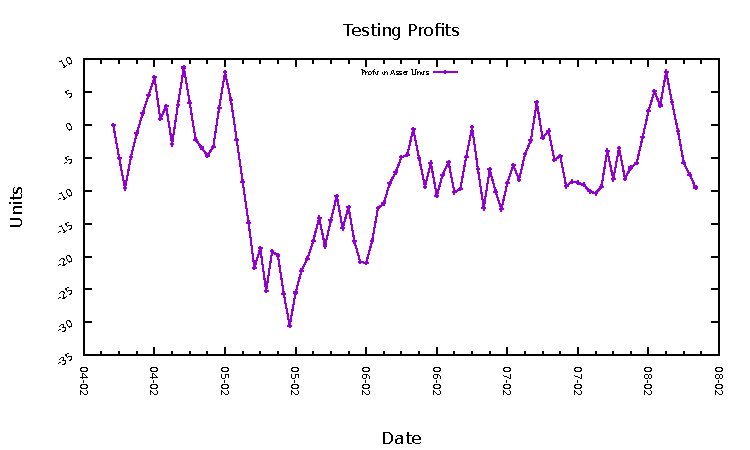
\includegraphics[width=.45\textwidth]{img/plots/aud_usd_h1-4agents-4rules-4ind-100gen_testing_profits.pdf}

  \medskip

  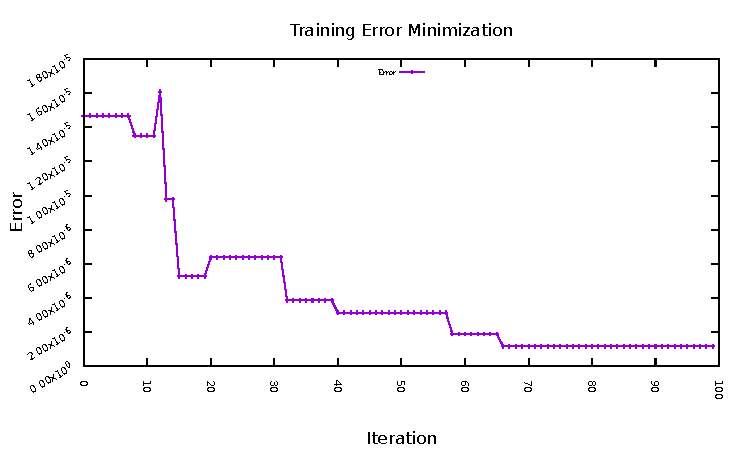
\includegraphics[width=.45\textwidth]{img/plots/aud_usd_h1-4agents-4rules-4ind-100gen_error_minimization.pdf}

  \caption{AUD/USD - 4 agents, 4 rules and 4 individuals}
  \label{figure:aud-usd-4agents-4rules-4individuals}
\end{figure}

\newpage

\subsection{AUD/USD 10 Agents, 10 Rules, 10 Individuals}
\label{results:forecast-aud-usd-10agents-10rules-10individuals}

The plots for the model generated using 10 agents with 10 rules each are shown
in Figure \ref{figure:aud-usd-10agents-10rules-10individuals}. It can be seen
that this model has better modelling capabilities than the 4 agents with 4 rules
each, as it performed better regarding profits in the training stage. However,
both models failed to obtain profits during the testing stage.

\begin{figure}[htp]
  \centering

  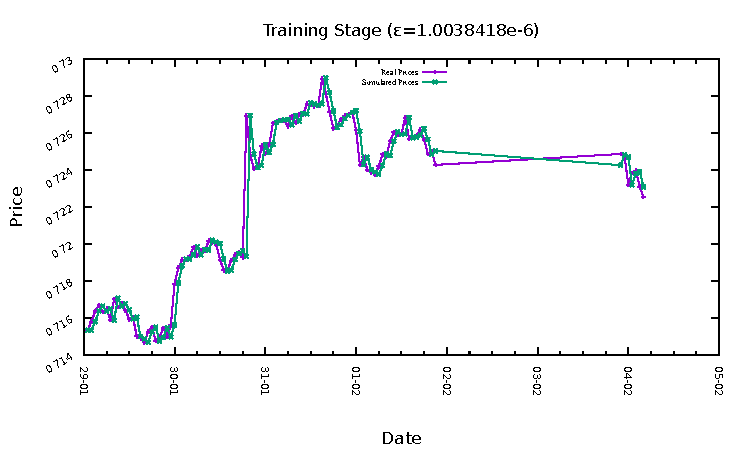
\includegraphics[width=.45\textwidth]{img/plots/aud_usd_h1-10agents-10rules-10ind-100gen_training_fit.pdf}\quad
  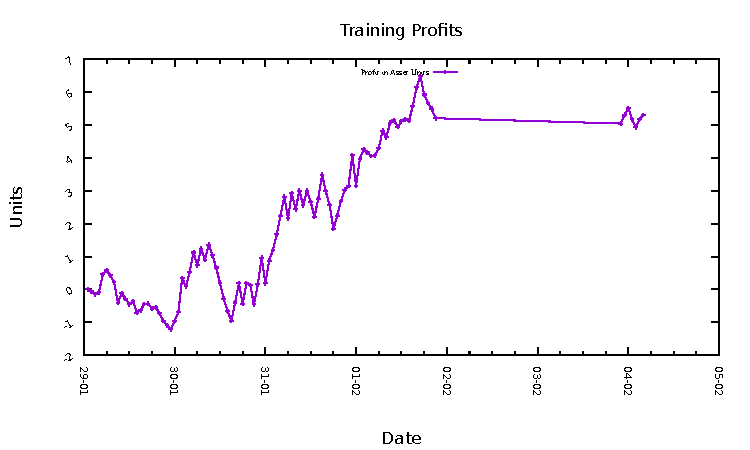
\includegraphics[width=.45\textwidth]{img/plots/aud_usd_h1-10agents-10rules-10ind-100gen_training_profits.pdf}

  \medskip

  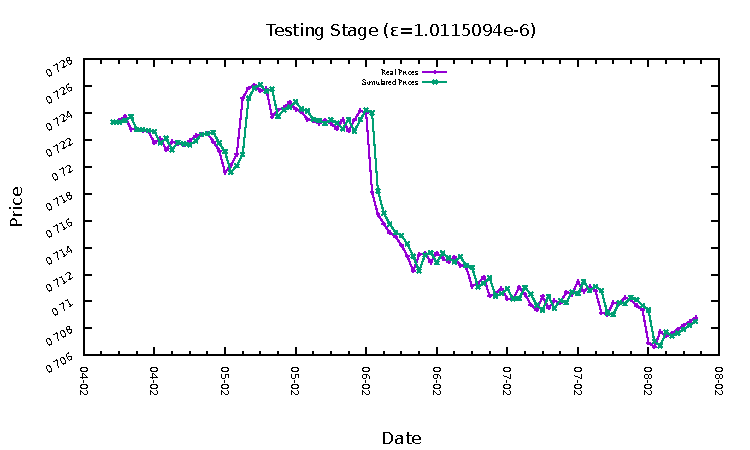
\includegraphics[width=.45\textwidth]{img/plots/aud_usd_h1-10agents-10rules-10ind-100gen_testing_fit.pdf}\quad
  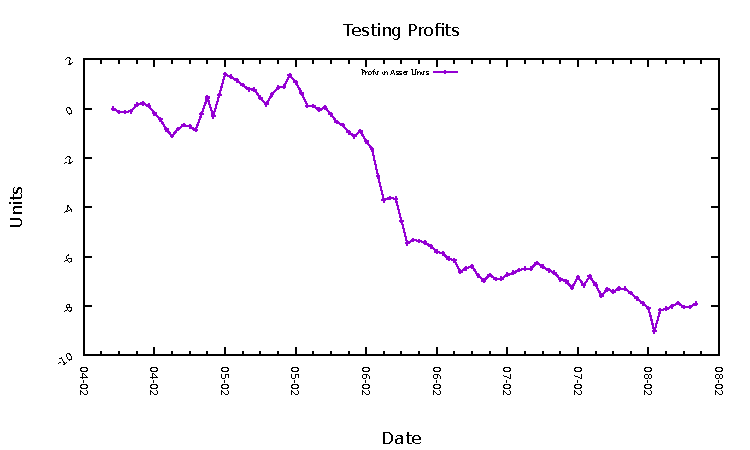
\includegraphics[width=.45\textwidth]{img/plots/aud_usd_h1-10agents-10rules-10ind-100gen_testing_profits.pdf}

  \medskip

  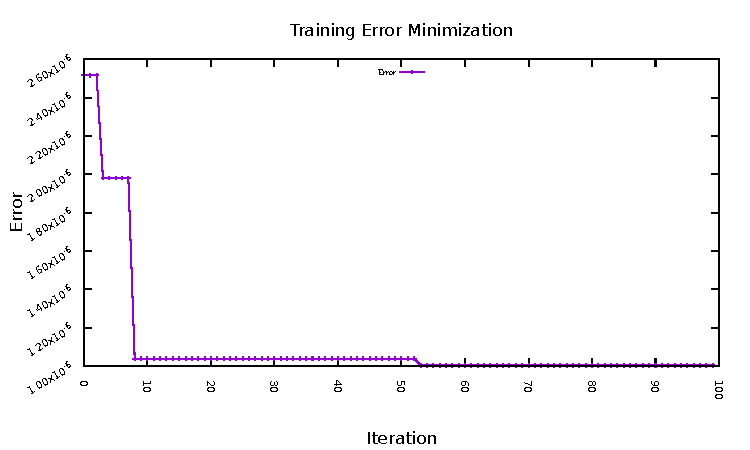
\includegraphics[width=.45\textwidth]{img/plots/aud_usd_h1-10agents-10rules-10ind-100gen_error_minimization.pdf}

  \caption{AUD/USD - 10 agents, 10 rules and 10 individuals}
  \label{figure:aud-usd-10agents-10rules-10individuals}
\end{figure}

\newpage

\subsection{AUD/USD 20 Agents, 20 Rules, 20 Individuals}
\label{results:forecast-aud-usd-20agents-20rules-20individuals}

Despite the increased modelling capabilities and diversity for the genetic
algorithm, the model generated by using 20 agents, 20 rules and 20 individuals
could not outperform the other two models for the AUD/USD. An explanation for
this is that the patterns present in the training dataset are notably different
than those found in the testing dataset, as it can be seen in Figure
\ref{figure:aud-usd-20agents-20rules-20individuals}.

\begin{figure}[htp]
  \centering

  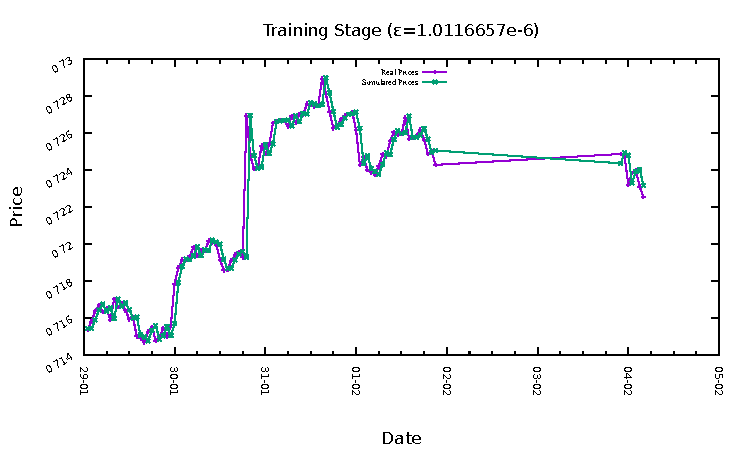
\includegraphics[width=.45\textwidth]{img/plots/aud_usd_h1-20agents-20rules-20ind-100gen_training_fit.pdf}\quad
  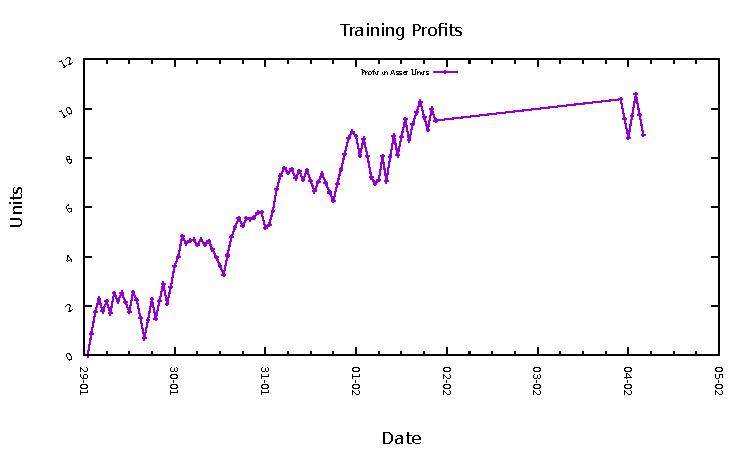
\includegraphics[width=.45\textwidth]{img/plots/aud_usd_h1-20agents-20rules-20ind-100gen_training_profits.pdf}

  \medskip

  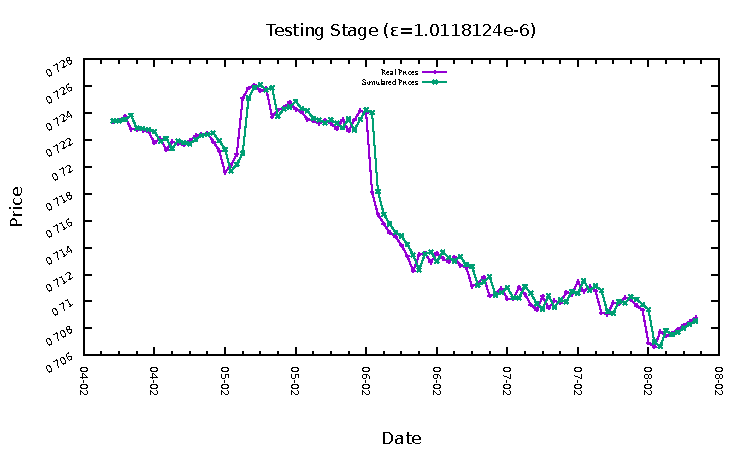
\includegraphics[width=.45\textwidth]{img/plots/aud_usd_h1-20agents-20rules-20ind-100gen_testing_fit.pdf}\quad
  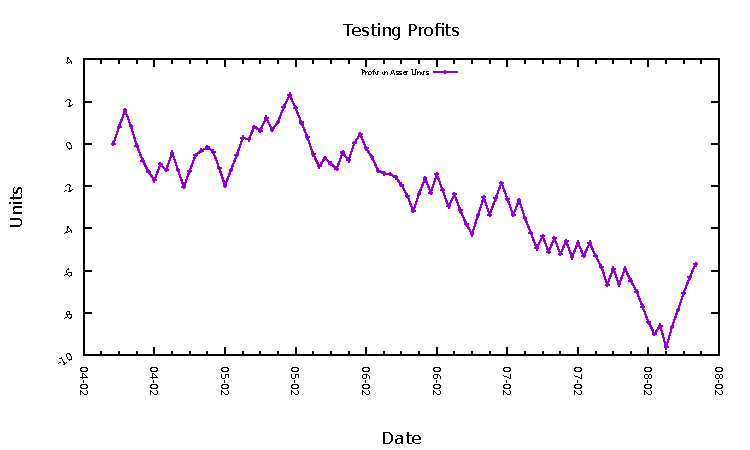
\includegraphics[width=.45\textwidth]{img/plots/aud_usd_h1-20agents-20rules-20ind-100gen_testing_profits.pdf}

  \medskip

  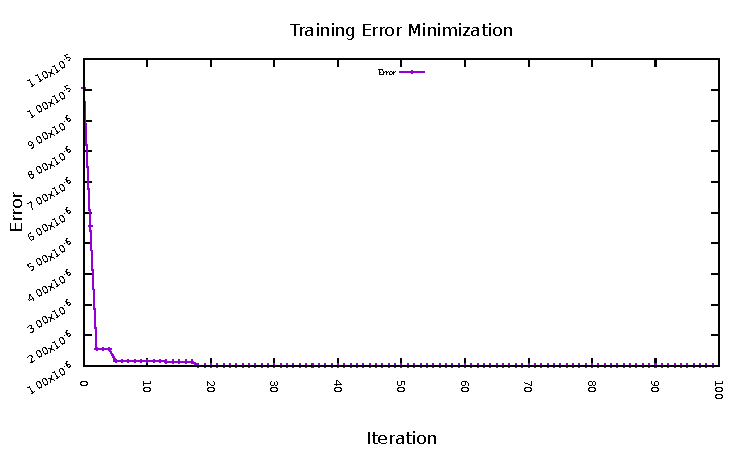
\includegraphics[width=.45\textwidth]{img/plots/aud_usd_h1-20agents-20rules-20ind-100gen_error_minimization.pdf}

  \caption{AUD/USD - 20 agents, 20 rules and 20 individuals}
  \label{figure:aud-usd-20agents-20rules-20individuals}
\end{figure}






\newpage

\subsection{EUR/GBP 4 Agents, 4 Rules, 4 Individuals}
\label{results:forecast-eur-gbp-4agents-4rules-4individuals}

Figure \ref{figure:aud-usd-20agents-20rules-20individuals} shows the plots for
the 4 agent, 4 rules, 4 individuals model. One can see that both profit plots
show bad performance. Although this is expected from this configuration, it can
also be seen that the model struggled in obtaining a simulation that resembled a
close representation of the real market, especially if it is compared to the 4
agents, 4 rules and 4 individual model for the AUD/USD market (see Figure
\ref{figure:eur-gbp-20agents-20rules-20individuals}).

\begin{figure}[htp]
  \centering

  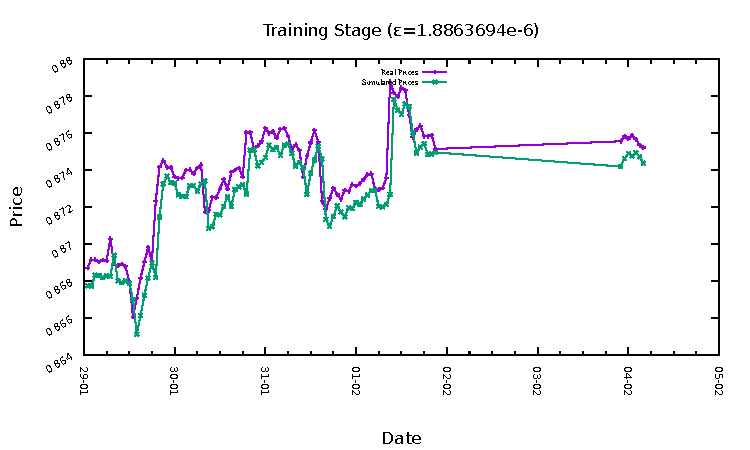
\includegraphics[width=.45\textwidth]{img/plots/eur_gbp_h1-4agents-4rules-4ind-100gen_training_fit.pdf}\quad
  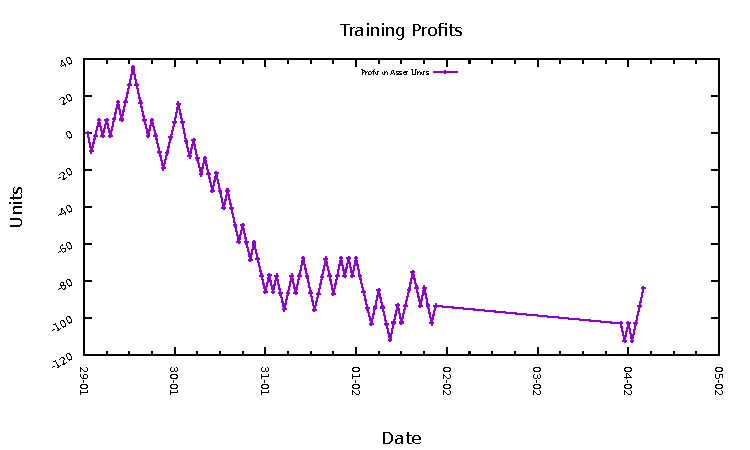
\includegraphics[width=.45\textwidth]{img/plots/eur_gbp_h1-4agents-4rules-4ind-100gen_training_profits.pdf}

  \medskip

  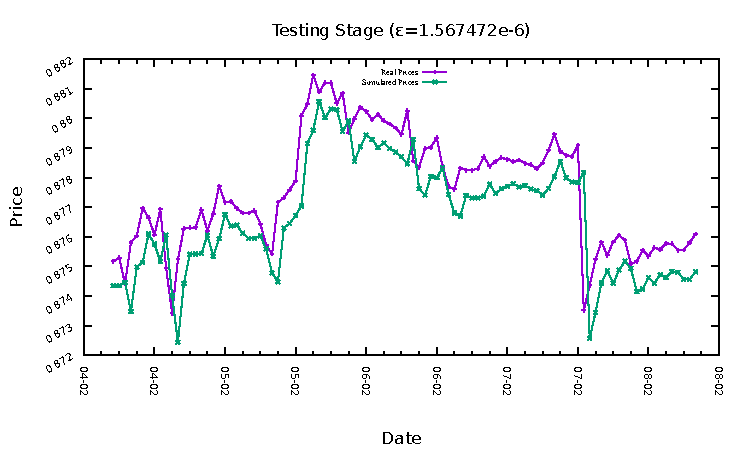
\includegraphics[width=.45\textwidth]{img/plots/eur_gbp_h1-4agents-4rules-4ind-100gen_testing_fit.pdf}\quad
  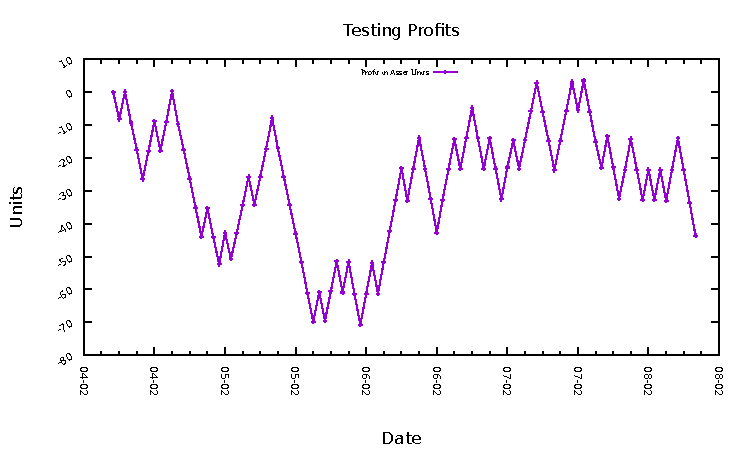
\includegraphics[width=.45\textwidth]{img/plots/eur_gbp_h1-4agents-4rules-4ind-100gen_testing_profits.pdf}

  \medskip

  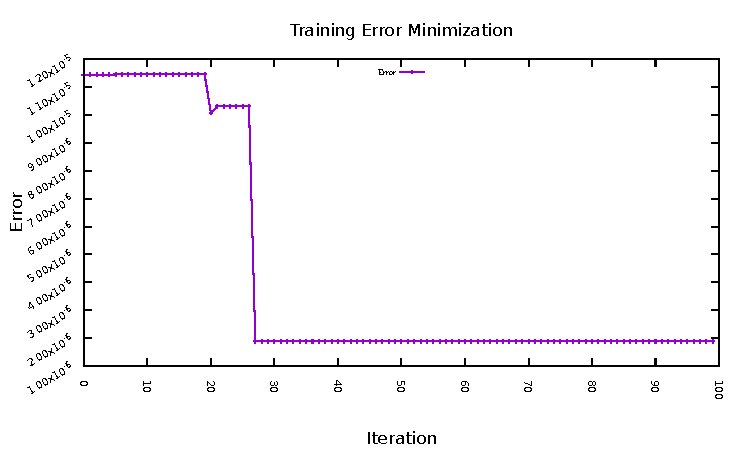
\includegraphics[width=.45\textwidth]{img/plots/eur_gbp_h1-4agents-4rules-4ind-100gen_error_minimization.pdf}

  \caption{EUR/GBP - 4 agents, 4 rules and 4 individuals}
  \label{figure:eur-gbp-4agents-4rules-4individuals}
\end{figure}

\newpage

\subsection{EUR/GBP 10 Agents, 10 Rules, 10 Individuals}
\label{results:forecast-eur-gbp-10agents-10rules-10individuals}

An interesting situation is presented in the plots in Figure
\ref{figure:eur-gbp-10agents-10rules-10individuals}. The profit plots are
identical in shape than the plots in Figure
\ref{figure:eur-gbp-4agents-4rules-4individuals}. The only inconsistency is the
magnitude of the trades, as the agents in the previous model traded more units
than the agents in this model.

\begin{figure}[htp]
  \centering

  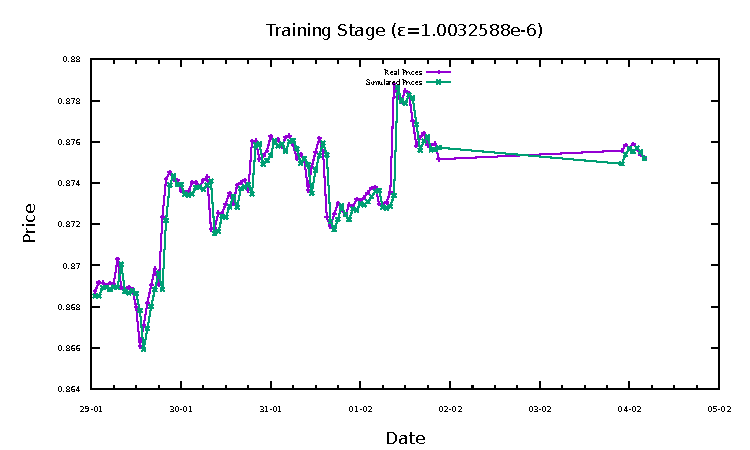
\includegraphics[width=.45\textwidth]{img/plots/eur_gbp_h1-10agents-10rules-10ind-100gen_training_fit.pdf}\quad
  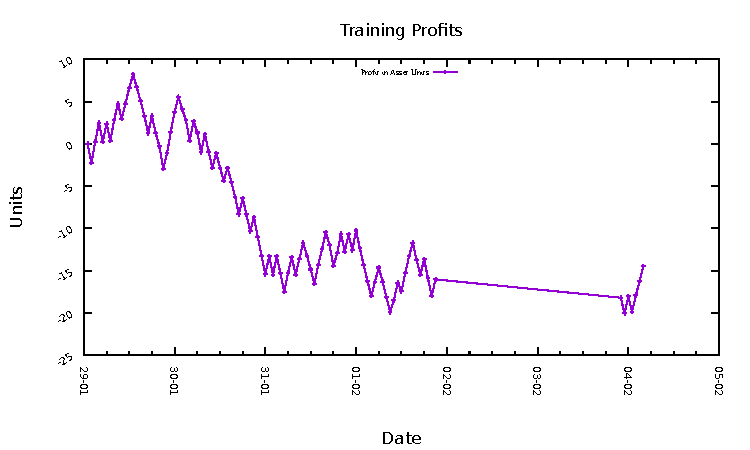
\includegraphics[width=.45\textwidth]{img/plots/eur_gbp_h1-10agents-10rules-10ind-100gen_training_profits.pdf}

  \medskip

  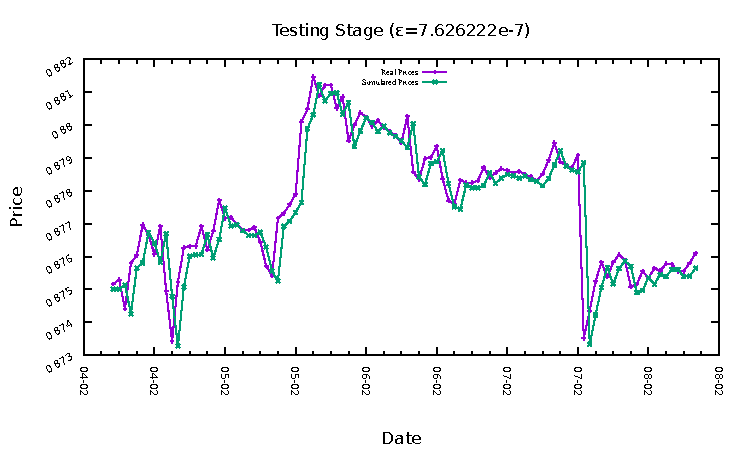
\includegraphics[width=.45\textwidth]{img/plots/eur_gbp_h1-10agents-10rules-10ind-100gen_testing_fit.pdf}\quad
  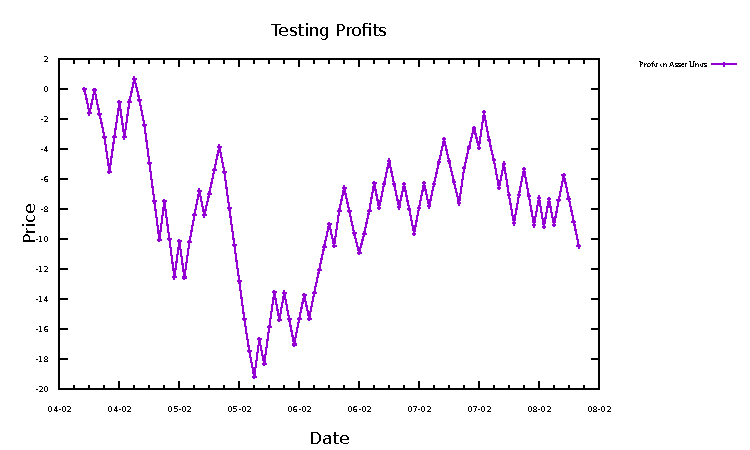
\includegraphics[width=.45\textwidth]{img/plots/eur_gbp_h1-10agents-10rules-10ind-100gen_testing_profits.pdf}

  \medskip

  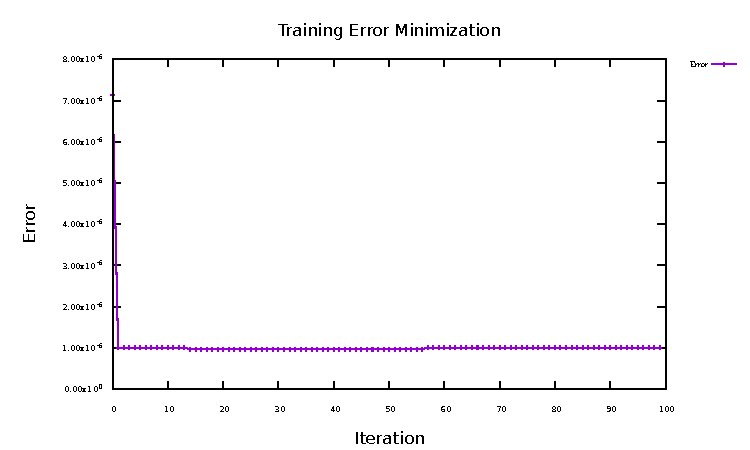
\includegraphics[width=.45\textwidth]{img/plots/eur_gbp_h1-10agents-10rules-10ind-100gen_error_minimization.pdf}

  \caption{EUR/GBP - 10 agents, 10 rules and 10 individuals}
  \label{figure:eur-gbp-10agents-10rules-10individuals}
\end{figure}

\newpage

\subsection{EUR/GBP 20 Agents, 20 Rules, 20 Individuals}
\label{results:forecast-eur-gbp-20agents-20rules-20individuals}

Although the model generated with these parameters performed well in the
training stage, as seen in Figure
\ref{figure:eur-gbp-20agents-20rules-20individuals}, it can be seen that the
model performed badly in the testing stage. However, it is worth mentioning that
the model performed well in the first 18-20 hours of the testing stage.

\begin{figure}[htp]
  \centering

  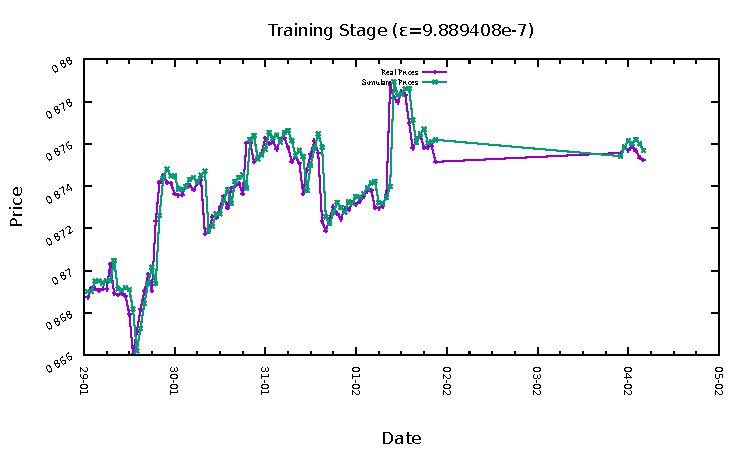
\includegraphics[width=.45\textwidth]{img/plots/eur_gbp_h1-20agents-20rules-20ind-100gen_training_fit.pdf}\quad
  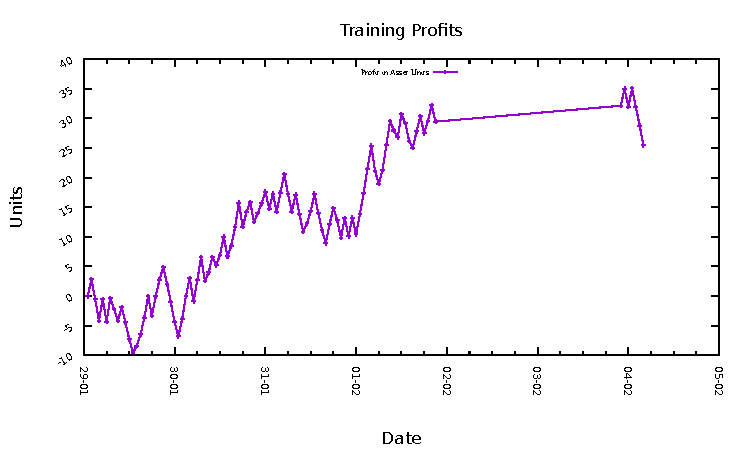
\includegraphics[width=.45\textwidth]{img/plots/eur_gbp_h1-20agents-20rules-20ind-100gen_training_profits.pdf}

  \medskip

  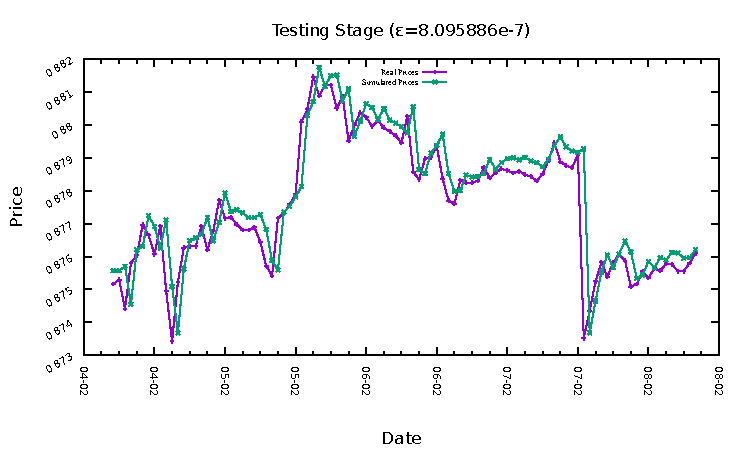
\includegraphics[width=.45\textwidth]{img/plots/eur_gbp_h1-20agents-20rules-20ind-100gen_testing_fit.pdf}\quad
  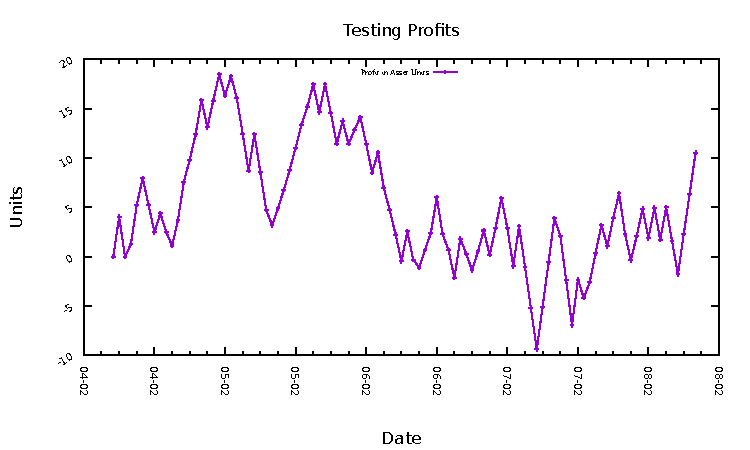
\includegraphics[width=.45\textwidth]{img/plots/eur_gbp_h1-20agents-20rules-20ind-100gen_testing_profits.pdf}

  \medskip

  \includegraphics[width=.45\textwidth]{img/plots/eur_gbp_h1-20agents-20rules-20ind-100gen_error_minimization.pdf}

  \caption{EUR/GBP - 20 agents, 20 rules and 20 individuals}
  \label{figure:eur-gbp-20agents-20rules-20individuals}
\end{figure}




\newpage

\subsection{EUR/USD 4 Agents, 4 Rules, 4 Individuals}
\label{results:forecast-eur-usd-4agents-4rules-4individuals}

This model can be seen how badly it performed in the testing stage, as shown in
Figure \ref{figure:eur-usd-4agents-4rules-4individuals}. However, it performed
well in the training stage. It must also be noted that a bad performance can be
expected due to the differences in the patterns between the training and testing
datasets.

\begin{figure}[htp]
  \centering

  \includegraphics[width=.45\textwidth]{img/plots/eur_usd_h1-4agents-4rules-4ind-100gen_training_fit.pdf}\quad
  \includegraphics[width=.45\textwidth]{img/plots/eur_usd_h1-4agents-4rules-4ind-100gen_training_profits.pdf}

  \medskip

  \includegraphics[width=.45\textwidth]{img/plots/eur_usd_h1-4agents-4rules-4ind-100gen_testing_fit.pdf}\quad
  \includegraphics[width=.45\textwidth]{img/plots/eur_usd_h1-4agents-4rules-4ind-100gen_testing_profits.pdf}

  \medskip

  \includegraphics[width=.45\textwidth]{img/plots/eur_usd_h1-4agents-4rules-4ind-100gen_error_minimization.pdf}

  \caption{EUR/USD - 4 agents, 4 rules and 4 individuals}
  \label{figure:eur-usd-4agents-4rules-4individuals}
\end{figure}

\newpage

\subsection{EUR/USD 10 Agents, 10 Rules, 10 Individuals}
\label{results:forecast-eur-usd-10agents-10rules-10individuals}

The plots in Figure \ref{figure:eur-usd-10agents-10rules-10individuals}
demonstrate an improvement regarding the curve-fitting capabilities of the model
compared to the previous model for the EUR/USD market. This is surprising, given
the differences in patterns between the two datasets. Additionally, it can be
noted that the model performed well in both the training and testing stages,
despite the model performing badly in the last hours of the testing stage.

\begin{figure}[htp]
  \centering

  \includegraphics[width=.45\textwidth]{img/plots/eur_usd_h1-10agents-10rules-10ind-100gen_training_fit.pdf}\quad
  \includegraphics[width=.45\textwidth]{img/plots/eur_usd_h1-10agents-10rules-10ind-100gen_training_profits.pdf}

  \medskip

  \includegraphics[width=.45\textwidth]{img/plots/eur_usd_h1-10agents-10rules-10ind-100gen_testing_fit.pdf}\quad
  \includegraphics[width=.45\textwidth]{img/plots/eur_usd_h1-10agents-10rules-10ind-100gen_testing_profits.pdf}

  \medskip

  \includegraphics[width=.45\textwidth]{img/plots/eur_usd_h1-10agents-10rules-10ind-100gen_error_minimization.pdf}

  \caption{EUR/USD - 10 agents, 10 rules and 10 individuals}
  \label{figure:eur-usd-10agents-10rules-10individuals}
\end{figure}

\newpage

\subsection{EUR/USD 20 Agents, 20 Rules, 20 Individuals}
\label{results:forecast-eur-usd-20agents-20rules-20individuals}

The model represented by the plots in Figure
\ref{figure:eur-usd-20agents-20rules-20individuals} is seen to have performed
badly in both the training and testing stages. A possible explanation for this
behavior is that more generations would be required in order for the model to
extract a generalization of the market, as a consequence of the high number of
agents and rules.

\begin{figure}[htp]
  \centering

  \includegraphics[width=.45\textwidth]{img/plots/eur_usd_h1-20agents-20rules-20ind-100gen_training_fit.pdf}\quad
  \includegraphics[width=.45\textwidth]{img/plots/eur_usd_h1-20agents-20rules-20ind-100gen_training_profits.pdf}

  \medskip

  \includegraphics[width=.45\textwidth]{img/plots/eur_usd_h1-20agents-20rules-20ind-100gen_testing_fit.pdf}\quad
  \includegraphics[width=.45\textwidth]{img/plots/eur_usd_h1-20agents-20rules-20ind-100gen_testing_profits.pdf}

  \medskip

  \includegraphics[width=.45\textwidth]{img/plots/eur_usd_h1-20agents-20rules-20ind-100gen_error_minimization.pdf}

  \caption{EUR/USD - 20 agents, 20 rules and 20 individuals}
  \label{figure:eur-usd-20agents-20rules-20individuals}
\end{figure}




\newpage

\subsection{GBP/USD 4 Agents, 4 Rules, 4 Individuals}
\label{results:forecast-gbp-usd-4agents-4rules-4individuals}

As expected from a model with poor modelling capabilities, the profit plots in
Figure \ref{figure:gbp-usd-4agents-4rules-4individuals} show that the model was
not able to simulate the patterns of the GBP/USD market.

\begin{figure}[htp]
  \centering

  \includegraphics[width=.45\textwidth]{img/plots/gbp_usd_h1-4agents-4rules-4ind-100gen_training_fit.pdf}\quad
  \includegraphics[width=.45\textwidth]{img/plots/gbp_usd_h1-4agents-4rules-4ind-100gen_training_profits.pdf}

  \medskip

  \includegraphics[width=.45\textwidth]{img/plots/gbp_usd_h1-4agents-4rules-4ind-100gen_testing_fit.pdf}\quad
  \includegraphics[width=.45\textwidth]{img/plots/gbp_usd_h1-4agents-4rules-4ind-100gen_testing_profits.pdf}

  \medskip

  \includegraphics[width=.45\textwidth]{img/plots/gbp_usd_h1-4agents-4rules-4ind-100gen_error_minimization.pdf}

  \caption{GBP/USD - 4 agents, 4 rules and 4 individuals}
  \label{figure:gbp-usd-4agents-4rules-4individuals}
\end{figure}

\newpage

\subsection{GBP/USD 10 Agents, 10 Rules, 10 Individuals}
\label{results:forecast-gbp-usd-10agents-10rules-10individuals}

In the case of this model for the GBP/USD market, a remarkable performance can
be noticed in Figure \ref{figure:gbp-usd-10agents-10rules-10individuals} in the
profit plots for both the training and testing stages.

\begin{figure}[htp]
  \centering

  \includegraphics[width=.45\textwidth]{img/plots/gbp_usd_h1-10agents-10rules-10ind-100gen_training_fit.pdf}\quad
  \includegraphics[width=.45\textwidth]{img/plots/gbp_usd_h1-10agents-10rules-10ind-100gen_training_profits.pdf}

  \medskip

  \includegraphics[width=.45\textwidth]{img/plots/gbp_usd_h1-10agents-10rules-10ind-100gen_testing_fit.pdf}\quad
  \includegraphics[width=.45\textwidth]{img/plots/gbp_usd_h1-10agents-10rules-10ind-100gen_testing_profits.pdf}

  \medskip

  \includegraphics[width=.45\textwidth]{img/plots/gbp_usd_h1-10agents-10rules-10ind-100gen_error_minimization.pdf}

  \caption{GBP/USD - 10 agents, 10 rules and 10 individuals}
  \label{figure:gbp-usd-10agents-10rules-10individuals}
\end{figure}

\newpage

\subsection{GBP/USD 20 Agents, 20 Rules, 20 Individuals}
\label{results:forecast-gbp-usd-20agents-20rules-20individuals}

In contrast to other models using 20 agents with 20 rules each, the model
represented by the plots in Figure
\ref{figure:gbp-usd-20agents-20rules-20individuals} is shown to perform well in
both the training and testing stages regarding the accumulated profits, although
the profits do not reach a similar magnitude as the previous model.

\begin{figure}[htp]
  \centering

  \includegraphics[width=.45\textwidth]{img/plots/gbp_usd_h1-20agents-20rules-20ind-100gen_training_fit.pdf}\quad
  \includegraphics[width=.45\textwidth]{img/plots/gbp_usd_h1-20agents-20rules-20ind-100gen_training_profits.pdf}

  \medskip

  \includegraphics[width=.45\textwidth]{img/plots/gbp_usd_h1-20agents-20rules-20ind-100gen_testing_fit.pdf}\quad
  \includegraphics[width=.45\textwidth]{img/plots/gbp_usd_h1-20agents-20rules-20ind-100gen_testing_profits.pdf}

  \medskip

  \includegraphics[width=.45\textwidth]{img/plots/gbp_usd_h1-20agents-20rules-20ind-100gen_error_minimization.pdf}

  \caption{GBP/USD - 20 agents, 20 rules and 20 individuals}
  \label{figure:gbp-usd-20agents-20rules-20individuals}
\end{figure}







\newpage

\subsection{USD/CAD 4 Agents, 4 Rules, 4 Individuals}
\label{results:forecast-usd-cad-4agents-4rules-4individuals}

The plots in Figure \ref{figure:usd-cad-4agents-4rules-4individuals} present an
interesting situation: the model seems to perform badly regarding profits in the
training stage, but not in the testing stage. This behavior is clearer after
examining the plots of the training and testing datasets: one exhibits a
downtrend market direction, while the other shiftes to a clear uptrend. The
model learned how to perform badly in a downtrend market, but it performed well
in the testing stage because of the shift in direction.

\begin{figure}[htp]
  \centering

  \includegraphics[width=.45\textwidth]{img/plots/usd_cad_h1-4agents-4rules-4ind-100gen_training_fit.pdf}\quad
  \includegraphics[width=.45\textwidth]{img/plots/usd_cad_h1-4agents-4rules-4ind-100gen_training_profits.pdf}

  \medskip

  \includegraphics[width=.45\textwidth]{img/plots/usd_cad_h1-4agents-4rules-4ind-100gen_testing_fit.pdf}\quad
  \includegraphics[width=.45\textwidth]{img/plots/usd_cad_h1-4agents-4rules-4ind-100gen_testing_profits.pdf}

  \medskip

  \includegraphics[width=.45\textwidth]{img/plots/usd_cad_h1-4agents-4rules-4ind-100gen_error_minimization.pdf}

  \caption{USD/CAD - 4 agents, 4 rules and 4 individuals}
  \label{figure:usd-cad-4agents-4rules-4individuals}
\end{figure}

\newpage

\subsection{USD/CAD 10 Agents, 10 Rules, 10 Individuals}
\label{results:forecast-usd-cad-10agents-10rules-10individuals}

In contrast to the previous model, the model represented by the plots shown in
Figure \ref{figure:usd-cad-10agents-10rules-10individuals} performs badly in the
testing stage, most likely because of the nature of the training dataset which
sharply contrasts with the nature of the testing dataset.

\begin{figure}[htp]
  \centering

  \includegraphics[width=.45\textwidth]{img/plots/usd_cad_h1-10agents-10rules-10ind-100gen_training_fit.pdf}\quad
  \includegraphics[width=.45\textwidth]{img/plots/usd_cad_h1-10agents-10rules-10ind-100gen_training_profits.pdf}

  \medskip

  \includegraphics[width=.45\textwidth]{img/plots/usd_cad_h1-10agents-10rules-10ind-100gen_testing_fit.pdf}\quad
  \includegraphics[width=.45\textwidth]{img/plots/usd_cad_h1-10agents-10rules-10ind-100gen_testing_profits.pdf}

  \medskip

  \includegraphics[width=.45\textwidth]{img/plots/usd_cad_h1-10agents-10rules-10ind-100gen_error_minimization.pdf}

  \caption{USD/CAD - 10 agents, 10 rules and 10 individuals}
  \label{figure:usd-cad-10agents-10rules-10individuals}
\end{figure}

\newpage

\subsection{USD/CAD 20 Agents, 20 Rules, 20 Individuals}
\label{results:forecast-usd-cad-20agents-20rules-20individuals}

The model represented by the plots in Figure
\ref{figure:usd-cad-20agents-20rules-20individuals} performs similarly to the
previously discussed model. The explanation behind this behavior should be the
same as the one mentioned in the previous Subsection.

\begin{figure}[htp]
  \centering

  \includegraphics[width=.45\textwidth]{img/plots/usd_cad_h1-20agents-20rules-20ind-100gen_training_fit.pdf}\quad
  \includegraphics[width=.45\textwidth]{img/plots/usd_cad_h1-20agents-20rules-20ind-100gen_training_profits.pdf}

  \medskip

  \includegraphics[width=.45\textwidth]{img/plots/usd_cad_h1-20agents-20rules-20ind-100gen_testing_fit.pdf}\quad
  \includegraphics[width=.45\textwidth]{img/plots/usd_cad_h1-20agents-20rules-20ind-100gen_testing_profits.pdf}

  \medskip

  \includegraphics[width=.45\textwidth]{img/plots/usd_cad_h1-20agents-20rules-20ind-100gen_error_minimization.pdf}

  \caption{USD/CAD - 20 agents, 20 rules and 20 individuals}
  \label{figure:usd-cad-20agents-20rules-20individuals}
\end{figure}



\newpage

\section{Extracting Insights about a Financial Market}
\label{section:extracting-insights-about-a-financial-market}

This Section shows interpretations of two different foreign exchange markets
obtained by examining the agents in the agent-based models generated for the
experiments shown in Section
\ref{section:forecasting-the-prices-of-a-financial-market}. Only the two markets
are presented in this Section as they are enough to demonstrate their use. The
rest of the interpretetations for the markets described in Section
\ref{section:forecasting-the-prices-of-a-financial-market} can be found in
Appendix \ref{app:market-interpretations}, and the full list of interpretations
for all the experiments performed can be found in the git repository of this
thesis document. The interpretations
consist of a series of sentences, where each give a summary of the profits,
perceptions, hesitancy and actions of groups of agents. Considering the
following sentence: ``3 agents — with an average profit of 68 units — perceived
in 85\% of the market that a weak resistance above current price — with a
hesitancy of 0.147 — is a signal to sell — with a hesitancy of 0.079.'', one can
draw the following conclusions about 3 agents in a community of agents: their
average profit in a dataset is of 68 units; in 85\% of the data points in the
dataset, they perceived that a price area with a low weight above the current
price is a signal to sell; after perceiving a low weight price area, they add
some hesitancy or doubt to their perception, and then they decide to sell, but
this decision has also some hesitancy or doubt. Hesitancy or doubt (see Section
\ref{section:using-the-agent-based-model-to-generate-insights-about-a-financial-market})
in this case is an indicative of how significant the perception has to be in
order to be indeed perceived as a low weight price area, and how many units are
actually traded; it can be seen as penalties to the agent's perception and
action.

The following interpretations show five sentences for the training stage of the
model and five sentences for the testing stage. These only represent excerpts of
the generated interpretations; it was decided for them to be truncated due to
space constraints in this thesis document, but the reader can find the full
interpretations in this thesis' Git repository. In order to obtain these five
sentence excerpts, all the generated sentences were ordered by the number of
agents and then by the number of units in profits. This way the sentences show
where the most number of agents in the community of agents coincided in their
perceptions and decisions, and then show what situations were the more
profitable.

%% Interpretations for the five foreign exchange markets AUD/USD, EUR/GBP, EUR/USD,
%% GBP/USD and USD/CAD are included. Each of these markets show interpretations for
%% the models with the following variants in parameters: 4 agents, 4 rules and 4
%% individuals; 10 agents, 10 rules and 10 individuals; 20 agents, 20 rules and 20
%% individuals.

\subsection{AUD/USD 4 Agents, 4 Rules, 4 Individuals}

One can see in the first sentence of the training set that 3 agents decided to
trade when a weak resistance is presented above the current price. In the
training stage these agents were not profitable, while in the testing stage they
were profitable. This indicates that this pattern is not as reliable as, for
example, the one presented in the second sentence in the training set, where
agents decided to buy when they perceived a weak resistance nearby the current
price. This behavior showed to also be profitable in the testing stage, as is
shown in the fourth sentence of the corresponding set.

\subsubsection{Training}

{\small
  \begin{itemize}
  \item 3 agents — with an average profit of -68 units — perceived in 68\% of
    the market that a weak resistance above current price — with a hesitancy of
    0.147 — is a signal to sell — with a hesitancy of 0.079.
  \item 2 agents — with an average profit of 280 units — perceived in 46\% of
    the market that a weak resistance nearby current price — with a hesitancy of
    0.133 — is a signal to buy — with a hesitancy of 0.097.
  \item 2 agents — with an average profit of 280 units — perceived in 22\% of
    the market that a moderate resistance above current price — with a hesitancy
    of 0.15 — is a signal to buy — with a hesitancy of 0.113.
  \item 2 agents — with an average profit of 38 units — perceived in 56\% of the
    market that a weak resistance below current price — with a hesitancy of
    0.246 — is a signal to buy — with a hesitancy of 0.094.
  \item 2 agents — with an average profit of -41 units — perceived in 56\% of
    the market that a weak resistance below current price — with a hesitancy of
    0.009 — is a signal to sell — with a hesitancy of 0.132.
  \end{itemize}
}

\subsubsection{Testing}

{\small
  \begin{itemize}
  \item 3 agents — with an average profit of 68 units — perceived in 85\% of the
    market that a weak resistance above current price — with a hesitancy of
    0.147 — is a signal to sell — with a hesitancy of 0.079.
  \item 2 agents — with an average profit of 352 units — perceived in 47\% of
    the market that a moderate resistance below current price — with a hesitancy
    of 0.134 — is a signal to sell — with a hesitancy of 0.151.
  \item 2 agents — with an average profit of 323 units — perceived in 6\% of the
    market that a strong resistance below current price — with a hesitancy of
    0.098 — is a signal to sell — with a hesitancy of 0.024.
  \item 2 agents — with an average profit of 323 units — perceived in 55\% of
    the market that a weak resistance nearby current price — with a hesitancy of
    0.04 — is a signal to sell — with a hesitancy of 0.138.
  \item 2 agents — with an average profit of 309 units — perceived in 0\% of the
    market that a strong resistance above current price — with a hesitancy of
    0.127 — is a signal to sell — with a hesitancy of 0.14.
  \end{itemize}
}

\subsection{EUR/GBP 4 Agents, 4 Rules, 4 Individuals}

An interesting situation in these sets of interpretations is that the only
sentence in the training set that signals an actual trade action is among the
most profitable interpretations in the testing stage -- but with a 0\% of
perception in the market. This can also be seen as a signal to not follow the
behavior presented by this model, which agrees the profit plots of the model
presented in the previous Section.

\subsubsection{Training}

{\small
  \begin{itemize}
  \item 3 agents — with an average profit of 60 units — perceived in 56\% of the
    market that a weak resistance above current price — with a hesitancy of
    0.094 — is a signal to hold the current position — with a hesitancy of
    0.029.
  \item 3 agents — with an average profit of 31 units — perceived in 36\% of the
    market that a moderate resistance nearby current price — with a hesitancy of
    0.126 — is a signal to hold the current position — with a hesitancy of
    0.194.
  \item 3 agents — with an average profit of -44 units — perceived in 13\% of
    the market that a strong resistance below current price — with a hesitancy
    of 0.044 — is a signal to hold the current position — with a hesitancy of
    0.152.
  \item 2 agents — with an average profit of 105 units — perceived in 13\% of
    the market that a strong resistance below current price — with a hesitancy
    of 0.114 — is a signal to sell — with a hesitancy of 0.102.
  \item 2 agents — with an average profit of 105 units — perceived in 42\% of
    the market that a weak resistance nearby current price — with a hesitancy of
    0.105 — is a signal to hold the current position — with a hesitancy of
    0.048.
  \end{itemize}
}

\subsubsection{Testing}

{\small
  \begin{itemize}
  \item 3 agents — with an average profit of 34 units — perceived in 79\% of the
    market that a weak resistance above current price — with a hesitancy of
    0.094 — is a signal to hold the current position — with a hesitancy of
    0.029.
  \item 3 agents — with an average profit of 18 units — perceived in 33\% of the
    market that a moderate resistance nearby current price — with a hesitancy of
    0.126 — is a signal to hold the current position — with a hesitancy of
    0.194.
  \item 3 agents — with an average profit of -23 units — perceived in 0\% of the
    market that a strong resistance below current price — with a hesitancy of
    0.044 — is a signal to hold the current position — with a hesitancy of
    0.152.
  \item 2 agents — with an average profit of 60 units — perceived in 0\% of the
    market that a strong resistance below current price — with a hesitancy of
    0.114 — is a signal to sell — with a hesitancy of 0.102.
  \item 2 agents — with an average profit of 60 units — perceived in 57\% of the
    market that a weak resistance nearby current price — with a hesitancy of
    0.105 — is a signal to hold the current position — with a hesitancy of
    0.048.
  \end{itemize}
}

\section{Comparison with other Works}
\label{section:comparison-with-other-works}

This Section presents a set of works that share many similarities to the work
proposed in this thesis and that are comparable to it. Table \ref{table:results}
shows five different works that focus on forecasting a financial market and
yield a rate of return. The table columns show the work reference and its
authors; the technique used to perform the forecasting; the optimization
algorithm used, if any; the financial market type used; the percentage of profit
or rate of return after a number of trades; and the standard deviation for the
aforementioned rate of return. The purpose of this table is to showcase what are
normal values of performance when forecasting financial markets and not to
provide a concise comparison for the proposed method, as many factors do not
match among the different works shown in the table: the size of the dataset used
for training, the technique used, the parameters of the optimization algorithm,
the number of trades performed, the type of the financial market,
etc. Furthermore, the results shown in this Chapter had the purpose of
demonstrating how the proposed method behaves using different parameters and not
to obtain the maximum possible rate of return.

\begin{table}[ht]
\caption{Performance of different approaches to financial market forecasting}
\label{table:results}
\centering
\begin{tabular}{|c|c|c|c|c|c|}
\hline
Work                                         & Technique                  & Optim. Alg. & Market Type              & ROR & SD \\
\hline
\hline
\cite{Fernandez-Blanco2008} & TI            & Genetic algorithm         & Stock             & 76.13\%     & 14.15\%            \\
\hline
\cite{Korczak2015}          & Fuzzy MAS        & -                      & ForEx & 32.77\%     & 109.09\%           \\
\hline
\cite{Korczak2016}          & Fuzzy MAS        & Genetic algorithm      & ForEx & 223.08\%    & 385.7\%            \\
\hline
\cite{Barbosa2010}          & Ensemble MAS     & -                      & ForEx & 27.78\%     & 12.43\%            \\
\hline
\cite{Escobar2013}          & Fuzzy TI         & -                      & Stock             & 7.35\%      & 6.9\%              \\
\hline
Thesis             & Fuzzy MAS        & Genetic algorithm      & ForEx & 2.15\%      & 38.85\%  \\
\hline
\end{tabular}
\end{table}

The rate of returns shown in Table \ref{table:results} for the proposed method
were obtained by averaging the units of profit for all the models that used a
configuration of 10 agents, 10 rules and 10 individuals for the following
financial markets: AUD/USD, EUR/GBP, EUR/USD, GBP/USD and USD/CAD. These models
were chosen because this configuration showed a good performance, considering
only the results included in this thesis document; other configurations could
have achieved a better performance.
\chapter{Results}
\label{chapter:results}

\chapter{Future Work}
\label{chapter:future-work}
\chapter{Future Work}
\label{chapter:future-work}
\appendix
\setcounter{secnumdepth}{1}
\chapter{}

\section{Market Interpretations}
\label{app:market-interpretations}

\subsection{AUD/USD 10 Agents, 10 Rules, 10 Individuals}
\label{results:interpretation-aud-usd-10agents-10rules-10individuals}

%% The sets of interpretations for this model are seen to differ in their
%% profits. However, as can be read in the interpretations, most of the agents in
%% the testing stage suggest that no trade should be made in those market
%% conditions. The agents in the sentences 2, 3, 4 and 5 internally decided to
%% trade, as all the agents need to trade at least some number of units as is
%% required by the implementation. However, the agents learned to trade small
%% amounts of units in these situations, and this is interpreted as a signal to
%% hold the current position and not initiate any new trade.

\subsubsection{Training}

{\small
  \begin{itemize}
  \item 4 agents — with an average profit of 142 units — perceived in 32\% of
    the market that a moderate resistance above current price — with a hesitancy
    of 0.08 — is a signal to sell — with a hesitancy of 0.055.
  \item 4 agents — with an average profit of 115 units — perceived in 33\% of
    the market that a moderate resistance above current price — with a hesitancy
    of 0.111 — is a signal to buy — with a hesitancy of 0.044.
  \item 4 agents — with an average profit of 112 units — perceived in 28\% of
    the market that a moderate resistance above current price — with a hesitancy
    of 0.097 — is a signal to hold the current position — with a hesitancy of
    0.128.
  \item 4 agents — with an average profit of 110 units — perceived in 34\% of
    the market that a moderate resistance below current price — with a hesitancy
    of 0.073 — is a signal to hold the current position — with a hesitancy of
    0.241.
  \item 4 agents — with an average profit of 110 units — perceived in 63\% of
    the market that a weak resistance above current price — with a hesitancy of
    0.128 — is a signal to hold the current position — with a hesitancy of
    0.226.
  \end{itemize}
}

\subsubsection{Testing}

{\small
  \begin{itemize}
  \item 4 agents — with an average profit of -72 units — perceived in 1\% of the
    market that a strong resistance above current price — with a hesitancy of
    0.122 — is a signal to buy — with a hesitancy of 0.098.
  \item 4 agents — with an average profit of -72 units — perceived in 41\% of
    the market that a moderate resistance nearby current price — with a
    hesitancy of 0.168 — is a signal to hold the current position — with a
    hesitancy of 0.41.
  \item 4 agents — with an average profit of -134 units — perceived in 55\% of
    the market that a moderate resistance below current price — with a hesitancy
    of 0.073 — is a signal to hold the current position — with a hesitancy of
    0.241.
  \item 4 agents — with an average profit of -134 units — perceived in 85\% of
    the market that a weak resistance above current price — with a hesitancy of
    0.128 — is a signal to hold the current position — with a hesitancy of
    0.226.
  \item 4 agents — with an average profit of -134 units — perceived in 13\% of
    the market that a moderate resistance above current price — with a hesitancy
    of 0.097 — is a signal to hold the current position — with a hesitancy of
    0.128.
  \end{itemize}
}

\subsection{AUD/USD 20 Agents, 20 Rules, 20 Individuals}

%% The interpretations generated by this model are similar to those generated by
%% the previous model. Although most agents profitable situations in the training
%% stage, most lost their positions in the testing stage. However, 3 out of 5
%% sentences in the testing interpretations signal a hold in the current position,
%% which tell the user to not follow the model's behavior.

\subsubsection{Training}

{\small
  \begin{itemize}
  \item 4 agents — with an average profit of 201 units — perceived in 25\% of
    the market that a moderate resistance below current price — with a hesitancy
    of 0.22 — is a signal to buy — with a hesitancy of 0.068.
  \item 4 agents — with an average profit of 199 units — perceived in 20\% of
    the market that a strong resistance nearby current price — with a hesitancy
    of 0.088 — is a signal to buy — with a hesitancy of 0.107.
  \item 4 agents — with an average profit of 193 units — perceived in 26\% of
    the market that a moderate resistance above current price — with a hesitancy
    of 0.493 — is a signal to hold the current position — with a hesitancy of
    0.112.
  \item 4 agents — with an average profit of 183 units — perceived in 72\% of
    the market that a weak resistance above current price — with a hesitancy of
    0.114 — is a signal to buy — with a hesitancy of 0.096.
  \item 4 agents — with an average profit of 182 units — perceived in 11\% of
    the market that a strong resistance below current price — with a hesitancy
    of 0.092 — is a signal to buy — with a hesitancy of 0.104.
  \end{itemize}
}

\subsubsection{Testing}


{\small
  \begin{itemize}
  \item 4 agents — with an average profit of -12 units — perceived in 13\% of
    the market that a strong resistance below current price — with a hesitancy
    of 0.163 — is a signal to sell — with a hesitancy of 0.058.
  \item 4 agents — with an average profit of -28 units — perceived in 49\% of
    the market that a weak resistance nearby current price — with a hesitancy of
    0.079 — is a signal to buy — with a hesitancy of 0.093.
  \item 4 agents — with an average profit of -77 units — perceived in 85\% of
    the market that a weak resistance above current price — with a hesitancy of
    0.06 — is a signal to hold the current position — with a hesitancy of 0.095.
  \item 4 agents — with an average profit of -77 units — perceived in 12\% of
    the market that a strong resistance nearby current price — with a hesitancy
    of 0.047 — is a signal to hold the current position — with a hesitancy of
    0.092.
  \item 4 agents — with an average profit of -77 units — perceived in 13\% of
    the market that a strong resistance below current price — with a hesitancy
    of 0.066 — is a signal to hold the current position — with a hesitancy of
    0.102.
  \end{itemize}
}

\subsection{EUR/GBP 10 Agents, 10 Rules, 10 Individuals}
\label{results:interpretation-eur-gbp-10agents-10rules-10individuals}

%% In this case, all the interpretations show negative profits, which support the
%% idea of ignoring the model's behavior.

\subsubsection{Training}

{\small
  \begin{itemize}
  \item 4 agents — with an average profit of -69 units — perceived in 22\% of
    the market that a moderate resistance below current price — with a hesitancy
    of 0.103 — is a signal to buy — with a hesitancy of 0.205.
  \item 4 agents — with an average profit of -70 units — perceived in 12\% of
    the market that a strong resistance below current price — with a hesitancy
    of 0.106 — is a signal to hold the current position — with a hesitancy of
    0.108.
  \item 4 agents — with an average profit of -71 units — perceived in 12\% of
    the market that a strong resistance below current price — with a hesitancy
    of 0.103 — is a signal to sell — with a hesitancy of 0.053.
  \item 4 agents — with an average profit of -79 units — perceived in 38\% of
    the market that a moderate resistance above current price — with a hesitancy
    of 0.133 — is a signal to sell — with a hesitancy of 0.052.
  \item 4 agents — with an average profit of -100 units — perceived in 47\% of
    the market that a weak resistance nearby current price — with a hesitancy of
    0.143 — is a signal to sell — with a hesitancy of 0.082.
  \end{itemize}
}

\subsubsection{Testing}

{\small
  \begin{itemize}
  \item 4 agents — with an average profit of -39 units — perceived in 27\% of
    the market that a moderate resistance below current price — with a hesitancy
    of 0.103 — is a signal to buy — with a hesitancy of 0.205.
  \item 4 agents — with an average profit of -40 units — perceived in 0\% of the
    market that a strong resistance below current price — with a hesitancy of
    0.106 — is a signal to hold the current position — with a hesitancy of
    0.108.
  \item 4 agents — with an average profit of -41 units — perceived in 0\% of the
    market that a strong resistance below current price — with a hesitancy of
    0.103 — is a signal to sell — with a hesitancy of 0.053.
  \item 4 agents — with an average profit of -45 units — perceived in 18\% of
    the market that a moderate resistance above current price — with a hesitancy
    of 0.133 — is a signal to sell — with a hesitancy of 0.052.
  \item 4 agents — with an average profit of -57 units — perceived in 53\% of
    the market that a weak resistance nearby current price — with a hesitancy of
    0.143 — is a signal to sell — with a hesitancy of 0.082.
  \end{itemize}
}

\subsection{EUR/GBP 20 Agents, 20 Rules, 20 Individuals}


%% All the interpretation sentences that actually suggest to take a trade action in
%% the market, in both the training and testing sets, exhibit profits.

\subsubsection{Training}


{\small
  \begin{itemize}
  \item 4 agents — with an average profit of 157 units — perceived in 42\% of
    the market that a moderate resistance above current price — with a hesitancy
    of 0.212 — is a signal to sell — with a hesitancy of 0.054.
  \item 4 agents — with an average profit of 146 units — perceived in 15\% of
    the market that a strong resistance nearby current price — with a hesitancy
    of 0.28 — is a signal to hold the current position — with a hesitancy of
    0.038.
  \item 4 agents — with an average profit of 144 units — perceived in 32\% of
    the market that a moderate resistance below current price — with a hesitancy
    of 0.079 — is a signal to hold the current position — with a hesitancy of
    0.07.
  \item 4 agents — with an average profit of 141 units — perceived in 56\% of
    the market that a weak resistance below current price — with a hesitancy of
    0.066 — is a signal to sell — with a hesitancy of 0.049.
  \item 4 agents — with an average profit of 135 units — perceived in 56\% of
    the market that a weak resistance below current price — with a hesitancy of
    0.083 — is a signal to hold the current position — with a hesitancy of
    0.076.
  \end{itemize}
}

\subsubsection{Testing}


{\small
  \begin{itemize}
  \item 4 agents — with an average profit of 85 units — perceived in 17\% of the
    market that a moderate resistance above current price — with a hesitancy of
    0.212 — is a signal to sell — with a hesitancy of 0.054.
  \item 4 agents — with an average profit of 79 units — perceived in 7\% of the
    market that a strong resistance nearby current price — with a hesitancy of
    0.28 — is a signal to hold the current position — with a hesitancy of 0.038.
  \item 4 agents — with an average profit of 78 units — perceived in 30\% of the
    market that a moderate resistance below current price — with a hesitancy of
    0.079 — is a signal to hold the current position — with a hesitancy of 0.07.
  \item 4 agents — with an average profit of 76 units — perceived in 70\% of the
    market that a weak resistance below current price — with a hesitancy of
    0.066 — is a signal to sell — with a hesitancy of 0.049.
  \item 4 agents — with an average profit of 73 units — perceived in 70\% of the
    market that a weak resistance below current price — with a hesitancy of
    0.083 — is a signal to hold the current position — with a hesitancy of
    0.076.
  \end{itemize}
}




\subsection{EUR/USD 4 Agents, 4 Rules, 4 Individuals}


%% The only set of agents that is shown in both the training and testing sets of
%% interpretations for this model lost some units during the testing stage. This
%% means that if one decided to follow any of the top patterns in the training set,
%% it would have resulted in a loss.

\subsubsection{Training}


{\small
  \begin{itemize}
  \item 4 agents — with an average profit of 13 units — perceived in 21\% of the
    market that a moderate resistance above current price — with a hesitancy of
    0.072 — is a signal to hold the current position — with a hesitancy of
    0.089.
  \item 3 agents — with an average profit of 65 units — perceived in 33\% of the
    market that a moderate resistance nearby current price — with a hesitancy of
    0.037 — is a signal to sell — with a hesitancy of 0.279.
  \item 3 agents — with an average profit of 53 units — perceived in 21\% of the
    market that a moderate resistance above current price — with a hesitancy of
    0.155 — is a signal to sell — with a hesitancy of 0.093.
  \item 3 agents — with an average profit of 52 units — perceived in 66\% of the
    market that a weak resistance below current price — with a hesitancy of
    0.124 — is a signal to sell — with a hesitancy of 0.23.
  \item 3 agents — with an average profit of 29 units — perceived in 31\% of the
    market that a moderate resistance nearby current price — with a hesitancy of
    0.092 — is a signal to hold the current position — with a hesitancy of
    0.075.
  \end{itemize}
}

\subsubsection{Testing}


{\small
  \begin{itemize}
  \item 4 agents — with an average profit of 14 units — perceived in 16\% of the
    market that a moderate resistance above current price — with a hesitancy of
    0.072 — is a signal to hold the current position — with a hesitancy of
    0.089.
  \item 3 agents — with an average profit of 19 units — perceived in 46\% of the
    market that a moderate resistance nearby current price — with a hesitancy of
    0.092 — is a signal to hold the current position — with a hesitancy of
    0.075.
  \item 3 agents — with an average profit of -3 units — perceived in 20\% of the
    market that a weak resistance below current price — with a hesitancy of
    0.124 — is a signal to sell — with a hesitancy of 0.23.
  \item 3 agents — with an average profit of -7 units — perceived in 15\% of the
    market that a moderate resistance above current price — with a hesitancy of
    0.155 — is a signal to sell — with a hesitancy of 0.093.
  \item 3 agents — with an average profit of -22 units — perceived in 23\% of
    the market that a weak resistance below current price — with a hesitancy of
    0.063 — is a signal to hold the current position — with a hesitancy of
    0.092.
  \end{itemize}
}

\subsection{EUR/USD 10 Agents, 10 Rules, 10 Individuals}
\label{results:interpretation-eur-usd-10agents-10rules-10individuals}

%% This is another case where every set of agents in the training interpretation
%% set resulted in losing units, and as a consequence this model should not be
%% followed as a guideline for trading.

\subsubsection{Training}

{\small
  \begin{itemize}
  \item 4 agents — with an average profit of 0 units — perceived in 76\% of the
    market that a weak resistance below current price — with a hesitancy of
    0.051 — is a signal to hold the current position — with a hesitancy of
    0.056.
  \item 4 agents — with an average profit of -20 units — perceived in 9\% of the
    market that a strong resistance below current price — with a hesitancy of
    0.109 — is a signal to buy — with a hesitancy of 0.055.
  \item 4 agents — with an average profit of -24 units — perceived in 46\% of
    the market that a weak resistance nearby current price — with a hesitancy of
    0.115 — is a signal to buy — with a hesitancy of 0.044.
  \item 4 agents — with an average profit of -24 units — perceived in 27\% of
    the market that a strong resistance nearby current price — with a hesitancy
    of 0.097 — is a signal to sell — with a hesitancy of 0.038.
  \item 4 agents — with an average profit of -44 units — perceived in 47\% of
    the market that a weak resistance nearby current price — with a hesitancy of
    0.226 — is a signal to hold the current position — with a hesitancy of 0.13.
  \end{itemize}
}

\subsubsection{Testing}

{\small
  \begin{itemize}
  \item 4 agents — with an average profit of -3 units — perceived in 30\% of the
    market that a weak resistance below current price — with a hesitancy of
    0.051 — is a signal to hold the current position — with a hesitancy of
    0.056.
  \item 4 agents — with an average profit of -64 units — perceived in 9\% of the
    market that a strong resistance below current price — with a hesitancy of
    0.109 — is a signal to buy — with a hesitancy of 0.055.
  \item 4 agents — with an average profit of -79 units — perceived in 41\% of
    the market that a weak resistance nearby current price — with a hesitancy of
    0.115 — is a signal to buy — with a hesitancy of 0.044.
  \item 4 agents — with an average profit of -79 units — perceived in 11\% of
    the market that a strong resistance nearby current price — with a hesitancy
    of 0.097 — is a signal to sell — with a hesitancy of 0.038.
  \item 4 agents — with an average profit of -138 units — perceived in 42\% of
    the market that a weak resistance nearby current price — with a hesitancy of
    0.226 — is a signal to hold the current position — with a hesitancy of 0.13.
  \end{itemize}
}

\subsection{EUR/USD 20 Agents, 20 Rules, 20 Individuals}


%% This model presents another situation where the majority of the agents lost
%% units and is a signal to be ignore the resulting model.

\subsubsection{Training}


{\small
  \begin{itemize}
  \item 4 agents — with an average profit of -10 units — perceived in 21\% of
    the market that a strong resistance nearby current price — with a hesitancy
    of 0.347 — is a signal to sell — with a hesitancy of 0.067.
  \item 4 agents — with an average profit of -12 units — perceived in 18\% of
    the market that a moderate resistance below current price — with a hesitancy
    of 0.156 — is a signal to sell — with a hesitancy of 0.1.
  \item 4 agents — with an average profit of -12 units — perceived in 72\% of
    the market that a weak resistance above current price — with a hesitancy of
    0.077 — is a signal to buy — with a hesitancy of 0.217.
  \item 4 agents — with an average profit of -22 units — perceived in 46\% of
    the market that a weak resistance nearby current price — with a hesitancy of
    0.065 — is a signal to buy — with a hesitancy of 0.097.
  \item 4 agents — with an average profit of -29 units — perceived in 4\% of the
    market that a strong resistance above current price — with a hesitancy of
    0.103 — is a signal to sell — with a hesitancy of 0.068.
  \end{itemize}
}

\subsubsection{Testing}


{\small
  \begin{itemize}
  \item 4 agents — with an average profit of -30 units — perceived in 11\% of
    the market that a strong resistance nearby current price — with a hesitancy
    of 0.347 — is a signal to sell — with a hesitancy of 0.067.
  \item 4 agents — with an average profit of -35 units — perceived in 57\% of
    the market that a moderate resistance below current price — with a hesitancy
    of 0.156 — is a signal to sell — with a hesitancy of 0.1.
  \item 4 agents — with an average profit of -35 units — perceived in 93\% of
    the market that a weak resistance above current price — with a hesitancy of
    0.077 — is a signal to buy — with a hesitancy of 0.217.
  \item 4 agents — with an average profit of -67 units — perceived in 44\% of
    the market that a weak resistance nearby current price — with a hesitancy of
    0.065 — is a signal to buy — with a hesitancy of 0.097.
  \item 4 agents — with an average profit of -87 units — perceived in 0\% of the
    market that a strong resistance above current price — with a hesitancy of
    0.103 — is a signal to sell — with a hesitancy of 0.068.
  \end{itemize}
}





\subsection{GBP/USD 4 Agents, 4 Rules, 4 Individuals}


%% A single pattern shown in the training sentences resulted in profits. However,
%% due to the signal to hold the current position, this model should also be
%% ignored for trading purposes.

\subsubsection{Training}


{\small
  \begin{itemize}
  \item 3 agents — with an average profit of 88 units — perceived in 37\% of the
    market that a weak resistance nearby current price — with a hesitancy of
    0.055 — is a signal to hold the current position — with a hesitancy of
    0.105.
  \item 3 agents — with an average profit of -92 units — perceived in 29\% of
    the market that a moderate resistance above current price — with a hesitancy
    of 0.139 — is a signal to hold the current position — with a hesitancy of
    0.085.
  \item 3 agents — with an average profit of -155 units — perceived in 10\% of
    the market that a strong resistance above current price — with a hesitancy
    of 0.018 — is a signal to buy — with a hesitancy of 0.112.
  \item 3 agents — with an average profit of -156 units — perceived in 46\% of
    the market that a moderate resistance nearby current price — with a
    hesitancy of 0.107 — is a signal to buy — with a hesitancy of 0.125.
  \item 3 agents — with an average profit of -156 units — perceived in 46\% of
    the market that a moderate resistance nearby current price — with a
    hesitancy of 0.137 — is a signal to hold the current position — with a
    hesitancy of 0.108.
  \end{itemize}
}

\subsubsection{Testing}


{\small
  \begin{itemize}
  \item 3 agents — with an average profit of 169 units — perceived in 46\% of
    the market that a weak resistance nearby current price — with a hesitancy of
    0.055 — is a signal to hold the current position — with a hesitancy of
    0.105.
  \item 3 agents — with an average profit of -178 units — perceived in 13\% of
    the market that a moderate resistance above current price — with a hesitancy
    of 0.139 — is a signal to hold the current position — with a hesitancy of
    0.085.
  \item 3 agents — with an average profit of -300 units — perceived in 10\% of
    the market that a strong resistance above current price — with a hesitancy
    of 0.018 — is a signal to buy — with a hesitancy of 0.112.
  \item 3 agents — with an average profit of -302 units — perceived in 32\% of
    the market that a moderate resistance nearby current price — with a
    hesitancy of 0.107 — is a signal to buy — with a hesitancy of 0.125.
  \item 3 agents — with an average profit of -302 units — perceived in 32\% of
    the market that a moderate resistance nearby current price — with a
    hesitancy of 0.137 — is a signal to hold the current position — with a
    hesitancy of 0.108.
  \end{itemize}
}

\subsection{GBP/USD 10 Agents, 10 Rules, 10 Individuals}
\label{results:interpretation-gbp-usd-10agents-10rules-10individuals}

%% Considering the sentences 1 and 4 of the training set of interpretations, one
%% can conclude that it can be a good idea to buy whenever the price is stagnated
%% -- denoted by a strong resistance nearby the current price -- and when there is
%% only moderate resistance above the current price. This is supported by the
%% sentences 1 and 4 of the testing set of interpretations.

\subsubsection{Training}

{\small
  \begin{itemize}
  \item 4 agents — with an average profit of 52 units — perceived in 18\% of the
    market that a strong resistance nearby current price — with a hesitancy of
    0.047 — is a signal to buy — with a hesitancy of 0.138.
  \item 4 agents — with an average profit of 48 units — perceived in 32\% of the
    market that a moderate resistance above current price — with a hesitancy of
    0.155 — is a signal to hold the current position — with a hesitancy of
    0.084.
  \item 4 agents — with an average profit of 48 units — perceived in 42\% of the
    market that a moderate resistance below current price — with a hesitancy of
    0.098 — is a signal to hold the current position — with a hesitancy of
    0.133.
  \item 4 agents — with an average profit of 39 units — perceived in 32\% of the
    market that a moderate resistance above current price — with a hesitancy of
    0.154 — is a signal to buy — with a hesitancy of 0.085.
  \item 4 agents — with an average profit of 37 units — perceived in 59\% of the
    market that a weak resistance above current price — with a hesitancy of
    0.124 — is a signal to sell — with a hesitancy of 0.118.
  \end{itemize}
}

\subsubsection{Testing}

{\small
  \begin{itemize}
  \item 4 agents — with an average profit of 96 units — perceived in 24\% of the
    market that a strong resistance nearby current price — with a hesitancy of
    0.047 — is a signal to buy — with a hesitancy of 0.138.
  \item 4 agents — with an average profit of 88 units — perceived in 44\% of the
    market that a moderate resistance below current price — with a hesitancy of
    0.098 — is a signal to hold the current position — with a hesitancy of
    0.133.
  \item 4 agents — with an average profit of 87 units — perceived in 16\% of the
    market that a moderate resistance above current price — with a hesitancy of
    0.155 — is a signal to hold the current position — with a hesitancy of
    0.084.
  \item 4 agents — with an average profit of 62 units — perceived in 16\% of the
    market that a moderate resistance above current price — with a hesitancy of
    0.154 — is a signal to buy — with a hesitancy of 0.085.
  \item 4 agents — with an average profit of 58 units — perceived in 35\% of the
    market that a moderate resistance nearby current price — with a hesitancy of
    0.194 — is a signal to sell — with a hesitancy of 0.511.
  \end{itemize}
}

\subsection{GBP/USD 20 Agents, 20 Rules, 20 Individuals}


%% Due to all the most recurring patterns in the agents not being profitable in the
%% training set of interpretations, this model should not be profitable.

\subsubsection{Training}


{\small
  \begin{itemize}
  \item 4 agents — with an average profit of -118 units — perceived in 56\% of
    the market that a weak resistance above current price — with a hesitancy of
    0.054 — is a signal to hold the current position — with a hesitancy of
    0.104.
  \item 4 agents — with an average profit of -118 units — perceived in 44\% of
    the market that a weak resistance nearby current price — with a hesitancy of
    0.087 — is a signal to buy — with a hesitancy of 0.044.
  \item 4 agents — with an average profit of -160 units — perceived in 32\% of
    the market that a moderate resistance above current price — with a hesitancy
    of 0.175 — is a signal to hold the current position — with a hesitancy of
    0.111.
  \item 4 agents — with an average profit of -176 units — perceived in 57\% of
    the market that a weak resistance above current price — with a hesitancy of
    0.105 — is a signal to sell — with a hesitancy of 0.158.
  \item 4 agents — with an average profit of -190 units — perceived in 32\% of
    the market that a moderate resistance above current price — with a hesitancy
    of 0.233 — is a signal to buy — with a hesitancy of 0.074.
  \end{itemize}
}

\subsubsection{Testing}


{\small
  \begin{itemize}
  \item 4 agents — with an average profit of -227 units — perceived in 67\% of
    the market that a weak resistance above current price — with a hesitancy of
    0.054 — is a signal to hold the current position — with a hesitancy of
    0.104.
  \item 4 agents — with an average profit of -227 units — perceived in 41\% of
    the market that a weak resistance nearby current price — with a hesitancy of
    0.087 — is a signal to buy — with a hesitancy of 0.044.
  \item 4 agents — with an average profit of -309 units — perceived in 27\% of
    the market that a moderate resistance above current price — with a hesitancy
    of 0.175 — is a signal to hold the current position — with a hesitancy of
    0.111.
  \item 4 agents — with an average profit of -341 units — perceived in 63\% of
    the market that a weak resistance above current price — with a hesitancy of
    0.105 — is a signal to sell — with a hesitancy of 0.158.
  \item 4 agents — with an average profit of -368 units — perceived in 28\% of
    the market that a moderate resistance above current price — with a hesitancy
    of 0.233 — is a signal to buy — with a hesitancy of 0.074.
  \end{itemize}
}





\subsection{USD/CAD 4 Agents, 4 Rules, 4 Individuals}


%% The last sentence in the training set of interpretations show an unusually high
%% hesitancy in the perceptions of the agents. This can signify that the pattern
%% could end in the future, and a shift to a similar but different pattern can
%% emerge. This is supported by the sentence 2 in the testing set, which now show
%% that the agents held their position in this pattern. It is further supported by
%% the third sentence, which shows the same pattern, but resulted in the agents
%% losing units.

\subsubsection{Training}


{\small
  \begin{itemize}
  \item 4 agents — with an average profit of 25 units — perceived in 6\% of the
    market that a strong resistance above current price — with a hesitancy of
    0.157 — is a signal to buy — with a hesitancy of 0.104.
  \item 3 agents — with an average profit of 48 units — perceived in 41\% of the
    market that a weak resistance nearby current price — with a hesitancy of
    0.041 — is a signal to hold the current position — with a hesitancy of
    0.238.
  \item 3 agents — with an average profit of 37 units — perceived in 60\% of the
    market that a weak resistance above current price — with a hesitancy of
    0.093 — is a signal to hold the current position — with a hesitancy of
    0.239.
  \item 3 agents — with an average profit of 37 units — perceived in 60\% of the
    market that a weak resistance above current price — with a hesitancy of
    0.071 — is a signal to sell — with a hesitancy of 0.072.
  \item 3 agents — with an average profit of 14 units — perceived in 36\% of the
    market that a moderate resistance below current price — with a hesitancy of
    0.451 — is a signal to sell — with a hesitancy of 0.062.
  \end{itemize}
}

\subsubsection{Testing}


{\small
  \begin{itemize}
  \item 4 agents — with an average profit of -44 units — perceived in 17\% of
    the market that a strong resistance above current price — with a hesitancy
    of 0.157 — is a signal to buy — with a hesitancy of 0.104.
  \item 3 agents — with an average profit of 59 units — perceived in 18\% of the
    market that a moderate resistance below current price — with a hesitancy of
    0.106 — is a signal to hold the current position — with a hesitancy of
    0.045.
  \item 3 agents — with an average profit of -23 units — perceived in 19\% of
    the market that a moderate resistance below current price — with a hesitancy
    of 0.451 — is a signal to sell — with a hesitancy of 0.062.
  \item 3 agents — with an average profit of -64 units — perceived in 47\% of
    the market that a weak resistance above current price — with a hesitancy of
    0.093 — is a signal to hold the current position — with a hesitancy of
    0.239.
  \item 3 agents — with an average profit of -64 units — perceived in 47\% of
    the market that a weak resistance above current price — with a hesitancy of
    0.071 — is a signal to sell — with a hesitancy of 0.072.
  \end{itemize}
}

\subsection{USD/CAD 10 Agents, 10 Rules, 10 Individuals}
\label{results:interpretation-usd-cad-10agents-10rules-10individuals}

%% Following the actions in the interpretations found in the training set will
%% result in a loss of units during the testing stage. However, this is most likely
%% due to the strong difference in market direction between the testing and
%% training datasets.

\subsubsection{Training}

{\small
  \begin{itemize}
  \item 9 agents — with an average profit of 343 units — perceived in 49\% of
    the market that a moderate resistance nearby current price — with a
    hesitancy of 0.097 — is a signal to sell — with a hesitancy of 0.115.
  \item 9 agents — with an average profit of 273 units — perceived in 16\% of
    the market that a strong resistance nearby current price — with a hesitancy
    of 0.173 — is a signal to sell — with a hesitancy of 0.087.
  \item 8 agents — with an average profit of 439 units — perceived in 39\% of
    the market that a moderate resistance above current price — with a hesitancy
    of 0.131 — is a signal to sell — with a hesitancy of 0.24.
  \item 8 agents — with an average profit of 425 units — perceived in 7\% of the
    market that a strong resistance above current price — with a hesitancy of
    0.081 — is a signal to buy — with a hesitancy of 0.028.
  \item 8 agents — with an average profit of 401 units — perceived in 53\% of
    the market that a weak resistance below current price — with a hesitancy of
    0.233 — is a signal to hold the current position — with a hesitancy of
    0.124.
  \end{itemize}
}

\subsubsection{Testing}

{\small
  \begin{itemize}
  \item 9 agents — with an average profit of -483 units — perceived in 22\% of
    the market that a strong resistance nearby current price — with a hesitancy
    of 0.173 — is a signal to sell — with a hesitancy of 0.087.
  \item 9 agents — with an average profit of -607 units — perceived in 40\% of
    the market that a moderate resistance nearby current price — with a
    hesitancy of 0.097 — is a signal to sell — with a hesitancy of 0.115.
  \item 8 agents — with an average profit of -441 units — perceived in 74\% of
    the market that a weak resistance below current price — with a hesitancy of
    0.101 — is a signal to sell — with a hesitancy of 0.091.
  \item 8 agents — with an average profit of -442 units — perceived in 45\% of
    the market that a weak resistance above current price — with a hesitancy of
    0.083 — is a signal to sell — with a hesitancy of 0.073.
  \item 8 agents — with an average profit of -602 units — perceived in 44\% of
    the market that a weak resistance above current price — with a hesitancy of
    0.123 — is a signal to hold the current position — with a hesitancy of
    0.131.
  \end{itemize}
}

\subsection{USD/CAD 20 Agents, 20 Rules, 20 Individuals}


%% Similarly to the previous sets of interpretations, the interpretations found in
%% this Subsection will result in a loss of units. However, this is most likely due
%% to the strong difference in market direction between the testing and training
%% datasets.

\subsubsection{Training}


{\small
  \begin{itemize}
  \item 4 agents — with an average profit of -106 units — perceived in 56\% of
    the market that a weak resistance above current price — with a hesitancy of
    0.06 — is a signal to sell — with a hesitancy of 0.203.
  \item 4 agents — with an average profit of -106 units — perceived in 37\% of
    the market that a moderate resistance below current price — with a hesitancy
    of 0.077 — is a signal to sell — with a hesitancy of 0.125.
  \item 4 agents — with an average profit of -142 units — perceived in 38\% of
    the market that a moderate resistance below current price — with a hesitancy
    of 0.052 — is a signal to buy — with a hesitancy of 0.092.
  \item 4 agents — with an average profit of -160 units — perceived in 50\% of
    the market that a weak resistance below current price — with a hesitancy of
    0.049 — is a signal to sell — with a hesitancy of 0.079.
  \item 4 agents — with an average profit of -169 units — perceived in 11\% of
    the market that a strong resistance below current price — with a hesitancy
    of 0.178 — is a signal to sell — with a hesitancy of 0.194.
  \end{itemize}
}

\subsubsection{Testing}


{\small
  \begin{itemize}
  \item 4 agents — with an average profit of 433 units — perceived in 10\% of
    the market that a strong resistance below current price — with a hesitancy
    of 0.066 — is a signal to buy — with a hesitancy of 0.073.
  \item 4 agents — with an average profit of 432 units — perceived in 18\% of
    the market that a strong resistance nearby current price — with a hesitancy
    of 0.075 — is a signal to hold the current position — with a hesitancy of
    0.059.
  \item 4 agents — with an average profit of 420 units — perceived in 10\% of
    the market that a strong resistance below current price — with a hesitancy
    of 0.083 — is a signal to hold the current position — with a hesitancy of
    0.103.
  \item 4 agents — with an average profit of 413 units — perceived in 38\% of
    the market that a moderate resistance nearby current price — with a
    hesitancy of 0.124 — is a signal to hold the current position — with a
    hesitancy of 0.072.
  \item 4 agents — with an average profit of 412 units — perceived in 40\% of
    the market that a moderate resistance above current price — with a hesitancy
    of 0.063 — is a signal to buy — with a hesitancy of 0.115.
  \end{itemize}
}

%% \clearpage

%% % Naive-Bayes Boredom
%% \subsection{Naïve Bayes}

%% \subsubsection{Aburrimiento}

%% \clearpage
%% \FloatBarrier
%% % Naive-Bayes Distraction
%% \subsubsection{Distracción}

%% \clearpage
%% \FloatBarrier
%% % Naive-Bayes Excitement
%% \subsubsection{Entusiasmo}

%%% \chapter{Figures}

%% \vspace*{-3in}

%% % \begin{figure}
%% % \vspace{2.4in}
%% % \caption{Armadillo slaying lawyer.}
%% % \label{arm:fig1}
%% % \end{figure}
%% % \clearpage
%% % \newpage

%% % \begin{figure}
%% % \vspace{2.4in}
%% % \caption{Armadillo eradicating national debt.}
%% % \label{arm:fig2}
%% % \end{figure}
%% \clearpage
%% \newpage

%% This defines the bibliography file (main.bib) and the bibliography style.
%% If you want to create a bibliography file by hand, change the contents of
%% this file to a `thebibliography' environment.  For more information 
%% see section 4.3 of the LaTeX manual.
\begin{singlespace}
\bibliography{main}
\bibliographystyle{plain}
\end{singlespace}

\end{document}

